\documentclass[lang = cn, scheme = chinese, thmcnt = section]{elegantbook}
% elegantbook      设置elegantbook文档类
% lang = cn        设置中文环境
% scheme = chinese 设置标题为中文
% thmcnt = section 设置计数器


%% 1.封面设置

\title{运筹学 - 刁在筠 - 笔记}                % 文档标题

\author{若水}                        % 作者

\myemail{ethanmxzhou@163.com}       % 邮箱

\homepage{helloethanzhou.github.io} % 主页

\date{\today}                       % 日期

\logo{PiCreatures_happy.pdf}        % 设置Logo

\cover{阿基米德螺旋曲线.pdf}          % 设置封面图片

% 修改标题页的色带
\definecolor{customcolor}{RGB}{135, 206, 250} 
% 定义一个名为customcolor的颜色,RGB颜色值为(135, 206, 250)

\colorlet{coverlinecolor}{customcolor}     % 将coverlinecolor颜色设置为customcolor颜色

%% 2.目录设置
\setcounter{tocdepth}{3}  % 目录深度为3

%% 3.引入宏包
\usepackage[all]{xy}
\usepackage{bbm, svg, graphicx, float, extpfeil, amsmath, amssymb, mathrsfs, mathalpha, hyperref, physics, multirow}


%% 4.定义命令
\newcommand{\N}{\mathbb{N}}            % 自然数集合
\newcommand{\R}{\mathbb{R}}            % 实数集合
\newcommand{\C}{\mathbb{C}}  		   % 复数集合
\newcommand{\Q}{\mathbb{Q}}            % 有理数集合
\newcommand{\Z}{\mathbb{Z}}            % 整数集合
\newcommand{\sub}{\subset}             % 包含
\newcommand{\im}{\text{im }}           % 像
\newcommand{\lang}{\langle}            % 左尖括号
\newcommand{\rang}{\rangle}            % 右尖括号
\newcommand{\bs}{\boldsymbol}          % 向量加黑
% \newcommand{\dd}{\mathrm{d}}           % 微分d
\newcommand{\col}{\coloneqq}
\newcommand{\ee}[1]{\mathrm{e}^{#1}}
\newcommand{\dis}{\displaystyle}
\newcommand{\function}[5]{
	\begin{align*}
		#1:\begin{aligned}[t]
			#2 &\longrightarrow #3\\
			#4 &\longmapsto #5
		\end{aligned}
	\end{align*}
}                                     % 函数

\newcommand{\lhdneq}{%
	\mathrel{\ooalign{$\lneq$\cr\raise.22ex\hbox{$\lhd$}\cr}}} % 真正规子群

\newcommand{\rhdneq}{%
	\mathrel{\ooalign{$\gneq$\cr\raise.22ex\hbox{$\rhd$}\cr}}} % 真正规子群

\begin{document}
	
	\maketitle       % 创建标题页
	
	\frontmatter     % 开始前言部分
	
	\chapter*{致谢}
	
	\markboth{致谢}{致谢}
	
	\vspace*{\fill}
	\begin{center}
		
		\large{感谢 \textbf{ 勇敢的 } 自己}
		
	\end{center}
	\vspace*{\fill}
	
	\tableofcontents % 创建目录
	
	\mainmatter      % 开始正文部分

\chapter{线性规划}

\section{线性规划模型}

\begin{definition}{线性规划问题的一般形式}
	线性规划(Linear Programming, LP)问题的一般形式为
	\begin{align*}\label{线性规划问题的一般形式}
		& \text{min}  \quad z = c_1 x_1 + \cdots + c_n x_n\\
		& \text{s.t.} \;\, \quad \begin{cases}
			a_{11} x_1 + \cdots + a_{1n} x_n = b_1 \\
			\vdots \\
			a_{p1} x_1 + \cdots + a_{pn} x_n = b_p \\
			a_{p+1,1} x_1 + \cdots + a_{p+1,n} x_n \ge b_{p+1} \\
			\vdots \\
			a_{m1} x_1 + \cdots + a_{mn} x_n \ge b_m \\
			x_1,\cdots,x_q\ge 0
		\end{cases}\tag{*}
	\end{align*}
	其中$x_1,\cdots,x_n$为待定的 {\bf{决策变量}};系数$a_{ij}$构成的矩阵
	$$
	\bs{A}=\begin{pmatrix}
		a_{11} & \cdots & a_{1n}\\
		\vdots & \ddots & \vdots\\
		a_{m1} & \cdots & a_{mn}
	\end{pmatrix}
	$$
	称为 {\bf{约束矩阵}},其第$j$个列向量为$\bs{A}_j$;$z = c_1 x_1 + \cdots + c_n x_n$称为 {\bf{目标函数}};向量$\bs{c}=(c_1,\cdots,c_n)^T$称为 {\bf{价值向量}};向量$\bs{b}=(b_1,\cdots,b_m)^T$称为 {\bf{右端向量}};条件$x_1,\cdots,x_q\ge 0$称为 {\bf{非负约束}},其余决策变量$x_{q+1},\cdots,x_{n}$称为 {\bf{自由变量}}。满足线性规划问题(\ref{线性规划问题的一般形式})的向量$\bs{x}=(x_1,\cdots,x_n)^T$称为 {\bf{可行解}},所有可行解构成 {\bf{可行区域}}$D$。 对于给定LP问题,成立如下情况其一。
	\begin{enumerate}
		\item $D=\varnothing$:称该问题 {\bf{无解}} 或 {\bf{不可行}}。 
		\item $D\ne\varnothing$且目标函数在$D$上无界:称该问题 {\bf{无界}}。 
		\item $D\ne\varnothing$且目标函数在$D$上有界:称该问题 {\bf{存在最优解}}。 
	\end{enumerate}
\end{definition}

\begin{definition}{线性规划问题的规范形式}
	LP问题的规范形式为
	\begin{align*}\label{线性规划问题的规范形式}
		& \text{min}  \quad \bs{c}^T\bs{x}\\
		& \text{s.t.} \;\, \quad \begin{cases}
			\bs{A} \bs{x} \ge \bs{b}\\
			\bs{x} \ge \bs{0}
		\end{cases}\tag{**}
	\end{align*}
\end{definition}

\begin{definition}{线性规划问题的标准形式}
	LP问题的标准形式为
	\begin{align*}\label{线性规划问题的标准形式}
		& \text{min}  \quad \bs{c}^T\bs{x}\\
		& \text{s.t.} \;\, \quad \begin{cases}
			\bs{A} \bs{x} = \bs{b}\\
			\bs{x} \ge \bs{0}
		\end{cases}\tag{***}
	\end{align*}
\end{definition}

\begin{theorem}{线性规划问题的形式的等价性}
	$$
	\text{一般形式} \iff
	\text{规范形式} \iff
	\text{标准形式}
	$$
\end{theorem}

\begin{proof}
	只需证明
	\begin{align*}
		& \text{一般形式}\implies\text{规范形式}\\
		& \text{一般形式}\implies\text{标准形式}
	\end{align*}

	一般形式$\implies$规范形式:对于等式约束
	$$
	a_1 x_1 + \cdots + a_n x_n = b_n
	$$
	可等价表示为
	$$
	\begin{cases}
		a_1 x_1 + \cdots + a_n x_n \ge b_n\\
		(-a_1) x_1 + \cdots + (-a_n) x_n \ge (-b_n)
	\end{cases}
	$$
	对于自由变量$x$,可引入变量$x^+$与$x^-$,使得成立
	$$
	x=x^+-x^-,\qquad 
	x^+,x^-\ge 0
	$$
	
	一般形式$\implies$标准形式:对于不等式约束
	$$
	a_1 x_1 + \cdots + a_n x_n \ge b_n
	$$
	可引入{\bf{松弛变量}}$y$,使得成立
	$$
	a_1 x_1 + \cdots + a_n x_n - y = b_n,\qquad 
	y\ge 0
	$$
	对于自由变量$x$,可引入变量$x^+$与$x^-$,使得成立
	$$
	x=x^+-x^-,\qquad 
	x^+,x^-\ge 0
	$$
\end{proof}

\section{可行区域与基本可行解}

\subsection{图解法}

\begin{theorem}
	\begin{enumerate}
		\item LP问题的可行域$D$形成有界或无界的凸集。
		\item 如果LP问题存在最优解,那么最优解存在于$D$的某个顶点。
	\end{enumerate}
\end{theorem}

\subsection{可行区域的几何结构}

\begin{definition}{凸集}
	称集合$S\sub \R^n$为凸集,如果成立
	$$
	\forall \bs{x},\bs{y}\in S,\forall \lambda\in[0,1]\implies
	\lambda\bs{x}+(1-\lambda)\bs{y}\in S
	$$
\end{definition}

\begin{theorem}{可行域为凸集}{标准形式的可行域为凸集}
	LP问题的标准形式(\ref{线性规划问题的标准形式})的可行域
	$$
	D=\{ \bs{x}\in\R^n:\bs{A}\bs{x}=\bs{b},\bs{x}\ge \bs{0} \}
	$$
	为凸集。
\end{theorem}

\begin{proof}
	任取$\bs{x},\bs{y}\in D$,以及$\lambda\in [0,1]$,由于$\bs{x},\bs{y}\ge \bs{0}$,那么
	$$
	\lambda\bs{x}+(1-\lambda)\bs{y}\ge \bs{0}
	$$
	又由于$\bs{A}\bs{x}=\bs{b}$且$\bs{A}\bs{y}=\bs{b}$,那么
	$$
	\bs{A}(\lambda\bs{x}+(1-\lambda)\bs{y})=\bs{b}
	$$
	进而
	$$
	\lambda\bs{x}+(1-\lambda)\bs{y}\in D
	$$
	从而$D$为凸集。
\end{proof}

\begin{lemma}{凸集的交为凸集}{凸集的交为凸集}
	任意一族凸集的交为凸集。
\end{lemma}

\begin{proof}
	这几乎是显然的!
\end{proof}

\begin{definition}{超平面}
	对于非零向量$\bs{a}\in\R^n$与$b\in\R$,称集合
	$$
	H=\{ \bs{x}\in\R^n:\bs{a}^T\bs{x}=b \}
	$$
	为$\R^n$中的超平面。$H$将$\R^n$分为两个半空间
	$$
	H^+=\{ \bs{x}\in\R^n:\bs{a}^T\bs{x}\ge b \},\qquad 
	H^-=\{ \bs{x}\in\R^n:\bs{a}^T\bs{x}\le b \}
	$$
\end{definition}

\begin{lemma}{}{超平面为凸集}
	超平面与其分割的半空间为凸集。
\end{lemma}

\begin{proof}
	这几乎是显然的!
\end{proof}

\begin{definition}{多面凸集}
	定义$\R^n$中的多面凸集为集合
	$$
	S=\{ \bs{x}\in\R^n:\bs{a}_i^T\bs{x}=b_i,\bs{a}_j^T\bs{x}\ge b_j,1\le i \le p,p+1\le j \le p+q \}
	$$
\end{definition}

\begin{definition}{多面体}
	称非空有界多面凸集为多面体,
\end{definition}

\begin{theorem}{多面凸集为凸集}{多面凸集为凸集}
	多面凸集为凸集。
\end{theorem}

\begin{proof}
	由引理\ref{lem:凸集的交为凸集}与\ref{lem:超平面为凸集},命题得证!
\end{proof}

\begin{definition}{凸集的顶点}
	对于凸集$S\sub\R^n$,称$\bs{x}\in S$为其顶点,如果对于任意$\bs{y}\ne\bs{z}\in S$以及$\lambda\in [0,1]$,成立
	$$
	\bs{x}\ne \lambda \bs{y} + (1 - \lambda) \bs{z}
	$$
\end{definition}

\subsection{基本可行解与线性规划基本定理}

\begin{definition}{基本可行解}
	对于LP问题的标准形式
	\begin{align*}
		& \text{min}  \quad \bs{c}^T\bs{x}\\
		& \text{s.t.} \;\, \quad \begin{cases}
			\bs{A} \bs{x} = \bs{b}\\
			\bs{x} \ge \bs{0}
		\end{cases}
	\end{align*}
	其中$\bs{A}\in\R^{m\times n}$。假设可行域非空,因此不妨假设$\text{rank}(\bs{A})=m\le n$。令$\bs{A}=(\bs{B},\bs{N})$,$\bs{x}=(\bs{x}_B,\bs{x}_N)^T$与其对应,其中$\bs{B}$为$m$阶非退化方阵,因此原方程化为{\bf{典型方程}}
	$$
	\bs{Ax}=\bs{b}
	\iff \bs{Bx}_B+\bs{Nx}_N=\bs{b}
	\iff \bs{x}_B=\bs{B}^{-1}\bs{b}-\bs{B}^{-1}\bs{Nx}_N
	$$
	称$\bs{B}$为 {\bf{基}},$\bs{B}$中的列向量为{\bf{基向量}};称$\bs{x}_B$为{\bf{基变量}},$\bs{x}_N$为{\bf{非基变量}};称$\bs{x}=(\bs{B}^{-1}\bs{b},\bs{0})^T$为对应$\bs{B}$的{\bf{基本解}};若$\bs{B}^{-1}\bs{b}\ge\bs{0}$,则称 $\bs{x}=(\bs{B}^{-1}\bs{b},\bs{0})^T$为对应$\bs{B}$的{\bf{基本可行解}};若$\bs{B}^{-1}\bs{b}>\bs{0}$,则称 $\bs{x}=(\bs{B}^{-1}\bs{b},\bs{0})^T$为{\bf{非退化基本可行解}}。
\end{definition}

\begin{lemma}{}{基本可行解等价于线性无关}
	对于LP问题的标准形式
	\begin{align*}
		& \text{min}  \quad \bs{c}^T\bs{x}\\
		& \text{s.t.} \;\, \quad \begin{cases}
			\bs{A} \bs{x} = \bs{b}\\
			\bs{x} \ge \bs{0}
		\end{cases}
	\end{align*}
	其中$\bs{A}\in\R^{m\times n}$,且$\text{rank}(\bs{A})=m\le n$,如果$\overline{\bs{x}}$为可行解,且其正分量位置为$n_1,\cdots,n_k$,那么
	$$
	\overline{\bs{x}}\text{ 为基本可行解}
	\iff
	\bs{A}_{n_1},\cdots,\bs{A}_{n_k}\text{ 线性无关}
	$$
\end{lemma}

\begin{proof}
	不妨
	$$
	\overline{\bs{x}}=(\overline{x}_1,\cdots,\overline{x}_k,0,\cdots,0)^T,\qquad \overline{x}_i>0
	$$
	必要性显然!对于充分性,由于$\bs{A}_{n_1},\cdots,\bs{A}_{n_k}$线性无关,那么$k\le m$。由于$\overline{x}$为可行解,那么
	$$
	\sum_{i=1}^{k}\overline{x}_i\bs{A}_i=\bs{b}
	$$
	其中$\bs{A}_i$为$\bs{A}$的第$i$个列向量。如果$k=m$,那么$\bs{B}=(\bs{A}_1,\cdots,\bs{A}_k)$为基,$\overline{x}$为$\bs{B}$对应的基本可行解。如果$k<m$,那么存在(不妨设为)$A_{k+1},\cdots,A_m$,使得$\bs{B}=(\bs{A}_1,\cdots,\bs{A}_{m})$为基,$\overline{x}$为$\bs{B}$对应的基本可行解。
\end{proof}

\begin{theorem}{基本可行解$\iff$顶点}{基本可行解等价于顶点}
	对于LP问题的标准形式
	\begin{align*}
		& \text{min}  \quad \bs{c}^T\bs{x}\\
		& \text{s.t.} \;\, \quad \begin{cases}
			\bs{A} \bs{x} = \bs{b}\\
			\bs{x} \ge \bs{0}
		\end{cases}
	\end{align*}
	其中$\bs{A}\in\R^{m\times n}$,且$\text{rank}(\bs{A})=m\le n$,如果$\overline{\bs{x}}$为可行解,$D$为可行域,那么
	$$
	\overline{\bs{x}}\text{ 为基本可行解}
	\iff
	\overline{\bs{x}}\text{ 为 }D\text{ 的顶点}
	$$
\end{theorem}

\begin{proof}
	如果$\overline{\bs{x}}$不为基本可行解,不妨$\overline{\bs{x}}$的前$k$个分量为正,并记作$\overline{\bs{x}}=(\overline{x}_1,\cdots,\overline{x}_k,0,\cdots,0)^T$,那么由引理\ref{lem:基本可行解等价于线性无关},$\bs{A}_1,\cdots,\bs{A}_k$线性相关,其中$\bs{A}_i$为$\bs{A}$的第$i$个列向量,从而存在非零向量$\bs{y}=(y_1,\cdots,y_k,0,\cdots,0)^T$,使得成立
	$$
	\sum_{i=1}^{k}y_i\bs{A}_i=\bs{0}
	$$
	对于对于任意$\delta>0$,成立
	$$
	\sum_{i=1}^{k}(\overline{x}_i\pm\delta y_i)\bs{A}_i=\bs{b}
	$$
	因此取$\bs{u}=\overline{\bs{x}}+\delta\bs{y}$与$\bs{v}=\overline{\bs{x}}-\delta\bs{y}$,就成立$\bs{Au}=\bs{Av}=\bs{b}$。令$\delta$充分小,使得$\bs{u},\bs{v}\ge \bs{0}$,因此$\bs{u},\bs{v}\in D$。由于$\bs{y}\ne \bs{0}$,那么$\bs{u}\ne\bs{v}$。由于
	$$
	\overline{\bs{x}}=\frac{1}{2}\bs{u}+\frac{1}{2}\bs{v}
	$$
	那么$\overline{\bs{x}}$不为顶点。
	
	如果$\overline{\bs{x}}$不为$D$的顶点,那么存在$\bs{u}\ne\bs{v}\in D$与$0<\lambda<1$成立
	$$
	\overline{\bs{x}}=\lambda\bs{u}+(1-\lambda)\bs{v}
	$$
	其中$\overline{\bs{x}}=(\overline{x}_1,\cdots,\overline{x}_n)^T$且$\bs{u}=(u_1,\cdots,u_n)^T,\bs{v}=(v_1,\cdots,v_n)^T$。不妨$\overline{\bs{x}}$的前$k$个分量为正,又由于当$i\ge k+1$时,成立$\overline{x}_i=0$且$u_i,v_i\ge 0$,那么$u_i=v_i=0$。由于$\bs{Ax}=\bs{Ay}=\bs{b}$,那么
	$$
	\sum_{i=1}^{k}(u_i-v_i)\bs{A}_i=\bs{0}
	$$
	其中$\bs{A}_i$为$\bs{A}$的第$i$个列向量。由于$\bs{x}\ne\bs{y}$,那么存在$1\le i\le k$,使得成立$u_i\ne v_i$,从而$\bs{A}_1,\cdots,\bs{A}_k$线性相关。由引理\ref{lem:基本可行解等价于线性无关},$\overline{\bs{x}}$不为基本可行解。
\end{proof}

\begin{theorem}{基本可行解的存在性}{基本可行解的存在性}
	对于LP问题的标准形式
	\begin{align*}
		& \text{min}  \quad \bs{c}^T\bs{x}\\
		& \text{s.t.} \;\, \quad \begin{cases}
			\bs{A} \bs{x} = \bs{b}\\
			\bs{x} \ge \bs{0}
		\end{cases}
	\end{align*}
	其中$\bs{A}\in\R^{m\times n}$,且$\text{rank}(\bs{A})=m\le n$,如果存在可行解,那么存在基本可行解。
\end{theorem}

\begin{proof}
	任取可行解$\bs{x}=(x_1,\cdots,x_n)$,不妨其前$k$个分量为正。如果$\bs{A}$的前$k$个列向量$\bs{A}_1,\cdots,\bs{A}_k$线性无关,那么由引理\ref{lem:基本可行解等价于线性无关},$\bs{x}$为基本可行解。如果$\bs{A}_1,\cdots,\bs{A}_k$线性无关,那么存在非零向量$\bs{\delta}=(\delta_1,\cdots,\delta_n,0,\cdots,0)$,使得成立
	$$
	\sum_{i=1}^{k}\delta_i\bs{A}_i=\bs{0}
	$$
	因此
	$$
	\bs{A\delta}=\sum_{i=1}^{k}\delta_i\bs{A}_i=\bs{0}
	$$
	取
	$$
	\varepsilon=\min\left\{ \frac{x_i}{|\delta_i|}:\delta_i\ne 0,1\le i\le k \right\}
	$$
	那么$\bs{x}\pm\varepsilon\bs{\delta}\ge 0$。由于
	$$
	\bs{A}(\bs{x}\pm\varepsilon\bs{\delta})
	=\bs{A}\bs{x}\pm \varepsilon\bs{A}\bs{\delta}
	=\bs{b}
	$$
	从而$\bs{x}\pm\varepsilon\bs{\delta}$均为可行解。
	
	注意到存在$1\le i\le k$,使得成立或$x_i+\varepsilon\delta_i=0$,或$x_i-\varepsilon\delta_i=0$,从而得到可行解$\bs{x}+\varepsilon\bs{\delta}$与$\bs{x}-\varepsilon\bs{\delta}$之一,使得其非零分量数$\le k-1$。如果其仍不为基本可行解,重复上述过程。容易知道该过程有限,从而可得到基本可行解。
\end{proof}

\begin{theorem}{基本可行解的存在性}{基本可行解的存在性}
	对于LP问题的标准形式
	\begin{align*}
		& \text{min}  \quad \bs{c}^T\bs{x}\\
		& \text{s.t.} \;\, \quad \begin{cases}
			\bs{A} \bs{x} = \bs{b}\\
			\bs{x} \ge \bs{0}
		\end{cases}
	\end{align*}
	其中$\bs{A}\in\R^{m\times n}$,且$\text{rank}(\bs{A})=m\le n$,如果存在最优解,那么最优解在基本可行解处取到。
\end{theorem}

\begin{proof}
	假设$\bs{x}$为最优解,如果$\bs{x}$为基本可行解,那么问题得证;否则由定理\ref{thm:基本可行解的存在性},存在$\varepsilon>0$与$\bs{\delta}$,使得$\bs{x}\pm\varepsilon\bs{\delta}$均为可行解,且$\bs{x}+\varepsilon\bs{\delta}$与$\bs{x}-\varepsilon\bs{\delta}$之一的非零分量数比$\bs{x}$严格小。其目标函数为
	$$
	\bs{c}^T(\bs{x}\pm\varepsilon\bs{\delta})
	=\bs{c}^T\bs{x}\pm \varepsilon\bs{c}^T\bs{\delta}
	\ge \bs{c}^T\bs{x}
	$$
	从而$\varepsilon\bs{c}^T=0$,因而
	$$
	\bs{c}^T(\bs{x}\pm\varepsilon\bs{\delta})
	=\bs{c}^T\bs{x}
	$$
	由定理\ref{thm:基本可行解的存在性},重复上述过程,可得基本可行解$\overline{\bs{x}}$,使得成立$\bs{c}^T\overline{\bs{x}}=\bs{c}^T \bs{x}$,进而最优解在基本可行解处取到。
\end{proof}

\section{单纯形方法}

\subsection{单纯形方法}

对于LP问题的标准形式
\begin{align*}
	& \text{min}  \quad \bs{c}^T\bs{x}\\
	& \text{s.t.} \;\, \quad \begin{cases}
		\bs{A} \bs{x} = \bs{b}\\
		\bs{x} \ge \bs{0}
	\end{cases}
\end{align*}
其中$\bs{A}\in\R^{m\times n}$,且$\text{rank}(\bs{A})=m\le n$,如果$\overline{\bs{x}}$为基本可行解,那么记其对应的基为$\bs{B}$,此时$\bs{Ax}=\bs{b}$化为
$$
\bs{x}_B+\bs{B}^{-1}\bs{Nx}_N=\bs{B}^{-1}\bs{b}
$$
不妨$\bs{B}=(\bs{A}_1,\cdots,\bs{A}_m)$,其中$\bs{A}_i$为$\bs{A}$的第$i$个列向量。记
\begin{align*}
	& \overline{\bs{A}}_i=\bs{B}^{-1}\bs{A}_i
	=(\overline{a}_{1i},\cdots,\overline{a}_{mi})^T,\qquad 
	1\le i\le n\\
	& \overline{\bs{b}}=\bs{B}^{-1}\bs{b}
	=(\overline{b}_{1},\cdots,\overline{b}_{m})^T
\end{align*}
那么
$$
\bs{x}_B+\sum_{i=m+1}^{n}x_i\overline{\bs{A}}_i=\overline{\bs{b}}
\qquad \text{或} \qquad
\bs{x}_B+\bs{B}^{-1}\bs{Nx}_N=\overline{\bs{b}}
$$
引入记号
$$
\zeta_i=\bs{c}_B^T\overline{\bs{A}}_i-c_i,\qquad 1\le i\le n
$$
或以向量表示
$$
\bs{\zeta}^T
=\bs{c}_B^T\bs{B}^{-1}\bs{A}-\bs{c}^T
=(\zeta_1,\cdots,\zeta_n)
=(\bs{\zeta}_B^T,\bs{\zeta}_N^T)
=(\bs{0},\bs{c}_B^T\bs{B}^{-1}\bs{N}-\bs{c}_N^T)
$$
目标函数化为
\begin{align*}
	\bs{c}^T\bs{x}
	& = \bs{c}_B^T\bs{x}_B+\bs{c}_N^T\bs{x}_N \\
	& = \bs{c}_B^T(\overline{\bs{b}}-\bs{B}^{-1}\bs{Nx}_N)+\bs{c}_N^T\bs{x}_N\\
	& = \bs{c}_B^T\overline{\bs{b}}- (\bs{c}_B^T\bs{B}^{-1}\bs{N}-\bs{c}_N^T)\bs{x}_N\\
	& = \bs{c}_B^T\overline{\bs{b}}-\sum_{i=m+1}^{n}(\bs{c}_B^T\overline{\bs{A}}_i-c_i)x_i\\
	& = \bs{c}_B^T\overline{\bs{b}}-\bs{\zeta}^T\bs{x}\\
	& = \bs{c}^T\overline{\bs{x}}-\bs{\zeta}^T\bs{x}
\end{align*}
从而原LP问题化为
\begin{align*}
	& \text{min}  \quad \bs{c}^T\overline{\bs{x}}-\bs{\zeta}^T\bs{x}\\
	& \text{s.t.} \;\, \quad \begin{cases}
		\bs{x}_B+\bs{B}^{-1}\bs{Nx}_N=\overline{\bs{b}}\\
		\bs{x} \ge \bs{0}
	\end{cases}
\end{align*}

\begin{theorem}{最优性准则}
	如果$\bs{\zeta}\le \bs{0}$,那么$\overline{\bs{x}}$为原LP问题的最优解。
\end{theorem}

\begin{proof}
	这当然是显然的!
\end{proof}

\begin{theorem}
	如果存在$m+1\le k\le n$,使得成立$\zeta_k>0$,且$\overline{\bs{A}}_k=\bs{B}^{-1}\bs{A}_k\ge \bs{0}$,那么原LP问题无界。
\end{theorem}

\begin{proof}
	令
	$$
	\bs{d}=\begin{pmatrix}
		-\overline{\bs{A}}_k\\\bs{0}
	\end{pmatrix}
	+\bs{e}_k
	$$
	其中$\bs{e}_k$为第$k$个分量为$1$,其余分量为$0$的$n$维向量。由于$\overline{\bs{A}}_k\le \bs{0}$,那么$\bs{d}\ge \bs{0}$,而
	\begin{align*}
		\bs{Ad}
		& = \begin{pmatrix}
			\bs{B} & \bs{N}
		\end{pmatrix}
		\begin{pmatrix}
			-\overline{\bs{A}}_k\\\bs{0}
		\end{pmatrix}
		+\bs{Ae}_k\\
		& = \begin{pmatrix}
			\bs{B} & \bs{N}
		\end{pmatrix}
		\begin{pmatrix}
			-\bs{B}^{-1}\bs{A}\\\bs{0}
		\end{pmatrix}
		+\begin{pmatrix}
			\bs{A}_1 & \cdots & \bs{A}_n
		\end{pmatrix}
		\begin{pmatrix}
			0 \\ \vdots \\ 0 \\ 1 \\ 0 \\ \vdots \\ 0
		\end{pmatrix}\\
		& = -\bs{A}_k+\bs{A}_k\\
		& = \bs{0}
	\end{align*}
	对于充分大的$\theta>0$,考察$\overline{\bs{x}}+\theta\bs{d}$,此时有
	$$
	\bs{A}(\overline{\bs{x}}+\theta\bs{d})
	=\bs{A}\overline{\bs{x}}+\theta\bs{A}\bs{d}
	=\bs{b},\qquad 
	\overline{\bs{x}}+\theta\bs{d}\ge\bs{0}
	$$
	因此$\overline{\bs{x}}+\theta\bs{d}$为原LP问题的可行解,其目标函数值为
	\begin{align*}
		\bs{c}^T(\overline{\bs{x}}+\theta\bs{d})
		& = \bs{c}^T\overline{\bs{x}}+\theta\bs{c}^T\bs{d}\\
		& = \bs{c}^T\overline{\bs{x}}
		+\theta\begin{pmatrix}
			\bs{c}_B^T & \bs{c}_N^T
		\end{pmatrix}
		\begin{pmatrix}
			-\overline{\bs{A}}_k \\ \bs{0}
		\end{pmatrix}
		+\theta\begin{pmatrix}
			c_1 & \cdots & c_n
		\end{pmatrix}
		\begin{pmatrix}
			0 \\ \vdots \\ 0 \\ 1 \\ 0 \\ \vdots \\ 0
		\end{pmatrix}\\
		& = \bs{c}^T\overline{\bs{x}}-\theta(\bs{c}_B^T\overline{\bs{A}}_k-c_k)\\
		& = \bs{c}^T\overline{\bs{x}}-\theta\zeta_k
	\end{align*}
	由于$\zeta_k>0$,而$\theta>0$可任意大,因此原LP问题无下界。
\end{proof}

\begin{theorem}
	对于非退化的基本可行解$\overline{\bs{x}}$,如果存在$m+1\le k\le n$,使得成立$\zeta_k>0$,且$\overline{\bs{A}}_k$中存在正分量,那么存在基本可行解$\hat{\bs{x}}$,使得成立$\bs{c}^T\hat{\bs{x}}<\bs{c}^T\overline{\bs{x}}$。
\end{theorem}

\begin{proof}
	令
	$$
	\bs{d}=\begin{pmatrix}
		-\overline{\bs{A}}_k\\\bs{0}
	\end{pmatrix}
	+\bs{e}_k
	$$
	其中$\bs{e}_k$为第$k$个分量为$1$,其余分量为$0$的$n$维向量。由于$\overline{\bs{A}}_k\le \bs{0}$,那么$\bs{d}\ge \bs{0}$,而
	\begin{align*}
		\bs{Ad}
		& = \begin{pmatrix}
			\bs{B} & \bs{N}
		\end{pmatrix}
		\begin{pmatrix}
			-\overline{\bs{A}}_k\\\bs{0}
		\end{pmatrix}
		+\bs{Ae}_k\\
		& = \begin{pmatrix}
			\bs{B} & \bs{N}
		\end{pmatrix}
		\begin{pmatrix}
			-\bs{B}^{-1}\bs{A}\\\bs{0}
		\end{pmatrix}
		+\begin{pmatrix}
			\bs{A}_1 & \cdots & \bs{A}_n
		\end{pmatrix}
		\begin{pmatrix}
			0 \\ \vdots \\ 0 \\ 1 \\ 0 \\ \vdots \\ 0
		\end{pmatrix}\\
		& = -\bs{A}_k+\bs{A}_k\\
		& = \bs{0}
	\end{align*}
	令
	$$
	\hat{\bs{x}}
	=\overline{\bs{x}}+\theta\bs{d}
	=\begin{pmatrix}
		\overline{\bs{b}} \\ \bs{0}
	\end{pmatrix}
	+\theta\begin{pmatrix}
		-\overline{\bs{A}}_k\\\bs{0}
	\end{pmatrix}
	+\theta\bs{e}_k
	=\begin{pmatrix}
		\overline{\bs{b}}-\theta\overline{\bs{A}}_k\\\bs{0}
	\end{pmatrix}
	+\theta\bs{e}_k
	$$
	容易知道
	$$
	\bs{A}\hat{\bs{x}}
	=\bs{A}\overline{\bs{x}}+\theta\bs{Ad}
	=\bs{b}
	$$
	取
	$$
	\theta
	=\min\left\{ \frac{\overline{b}_i}{\overline{a}_{ik}}:\overline{a}_{ik}>0,1\le i \le m \right\}
	=\frac{\overline{b}_r}{\overline{a}_{rk}}
	$$
	从而$\hat{\bs{x}}\ge \bs{0}$,进而$\hat{\bs{x}}$为可行解。
	
	考察$\hat{\bs{x}}$,其各分量为
	\begin{align*}
		& \hat{x}_i = \overline{b}_i-\frac{\overline{b}_r}{\overline{a}_{rk}}\overline{a}_{ik},\qquad 1\le i \le m,i\ne r\\
		& \hat{x}_i = 0,\qquad m+1\le i \le n,i\ne k\\
		& \hat{x}_r = 0\\
		& \hat{x}_k = \frac{\overline{b}_r}{\overline{a}_{rk}}
	\end{align*}
	若要证明$\hat{\bs{x}}$为基本可行解,由引理\ref{lem:基本可行解等价于线性无关},只需证明$\bs{A}_1,\cdots,\bs{A}_{r-1},\bs{A}_k,\bs{A}_{r+1},\cdots,\bs{A}_m$线性无关。若不然,$\bs{A}_1,\cdots,\bs{A}_{r-1},\bs{A}_k,\bs{A}_{r+1},\cdots,\bs{A}_m$线性相关,由于$\bs{A}_1,\cdots,\bs{A}_m$线性无关,因此向量$\bs{A}_k$可由其余$m-1$个向量线性表出,即存在$m-1$个数$y_i$,其中$1\le i\le m$且$i\ne r$,使得成立
	$$
	\bs{A}_k=\sum_{\substack{1\le i\le m\\i\ne r}}y_i\bs{A}_i
	$$
	又因为$\overline{\bs{A}}_k=\bs{B}^{-1}\bs{A}_k$,因此
	$$
	\bs{A}_k
	=\bs{B}\overline{\bs{A}}_k
	=\begin{pmatrix}
		\bs{A}_1 & \cdots & \bs{A}_m
	\end{pmatrix}
	\begin{pmatrix}
		\overline{a}_{1k}\\\vdots\\\overline{a}_{mk}
	\end{pmatrix}
	=\sum_{i=1}^{m}\overline{a}_{ik}\bs{A}_i
	$$
	两式作差
	$$
	\overline{a}_{rk}\bs{A}_r
	+\sum_{\substack{1\le i\le m\\i\ne r}}(\overline{a}_{ik}-y_i)\bs{A}_i
	=\bs{0}
	$$
	由于$\overline{a}_{rk}\ne 0$,因此$\bs{A}_1,\cdots,\bs{A}_m$线性相关,产生矛盾!进而$\hat{\bs{x}}$为基本可行解。
	
	由非退化假设$\overline{\bs{b}}>\bs{0}$,因此$\theta=\overline{b}_r/\overline{a}_{rk}>0$,从而
	\begin{align*}
		\bs{c}^T\hat{\bs{x}}
		& = \bs{c}^T(\overline{\bs{x}}+\theta\bs{d})\\
		& = \bs{c}^T\overline{\bs{x}}+\theta\bs{c}^T\bs{d}\\
		& = \bs{c}^T\overline{\bs{x}}
		+\theta\begin{pmatrix}
			\bs{c}_B^T & \bs{c}_N^T
		\end{pmatrix}
		\begin{pmatrix}
			-\overline{\bs{A}}_k \\ \bs{0}
		\end{pmatrix}
		+\theta\begin{pmatrix}
			c_1 & \cdots & c_n
		\end{pmatrix}
		\begin{pmatrix}
			0 \\ \vdots \\ 0 \\ 1 \\ 0 \\ \vdots \\ 0
		\end{pmatrix}\\
		& = \bs{c}^T\overline{\bs{x}}-\theta(\bs{c}_B^T\overline{\bs{A}}_k-c_k)\\
		& = \bs{c}^T\overline{\bs{x}}-\theta\zeta_k\\
		& <\bs{c}^T\overline{\bs{x}}
	\end{align*}
\end{proof}

\begin{theorem}{单纯形方法}
	\begin{enumerate}
		\item 选择基$\bs{B}$,使得对应$\bs{b}\ge 0$。
		\item 求出$\displaystyle \zeta_k=\max_{1\le i \le n}\zeta_i$。
		\item 若$\zeta_k\le 0$,停止,已找到最优解;否则转至第4步。
		\item 若$\overline{\bs{A}}_{\cdot,k}\le\bs{0}$,原问题无界;否则转至第5步。
		\item 求出$\displaystyle \frac{\overline{b}_r}{\overline{a}_{rk}}=\min\left\{ \frac{\overline{b}_i}{\overline{a}_{ik}}:\overline{a}_{ik}>0,1\le i \le m \right\}$。
		\item 以$\overline{a}_{rk}$为转轴元作旋转变换,转至第2步。
	\end{enumerate}
\end{theorem}

\begin{theorem}{对偶单纯形方法}
	\begin{enumerate}
		\item 选择基$\bs{B}$,使得对应$\bs{b}\le 0$。
		\item 求$\displaystyle \overline{b}_r=\min_{1\le i \le m}\overline{b}_i$。
		\item 若$\overline{b}_r\ge 0$,停止,已找到最优解;否则转至第4步。
		\item 若$\overline{\bs{A}}_{r,\cdot}\ge\bs{0}$,原问题无解;否则转至第5步。
		\item 求出$\displaystyle \frac{\zeta_k}{\overline{a}_{rk}}=\min\left\{ \frac{\zeta_j}{\overline{a}_{rj}}:\overline{a}_{rj}<0,1\le j \le n \right\}$。
		\item 以$\overline{a}_{rk}$为转轴元作旋转变换,转至第2步。
	\end{enumerate}
\end{theorem}

\begin{table}[H]
	\centering
	\begin{tabular}{cll}
		\toprule
		\textbf{序号} & \textbf{单纯形方法} & \textbf{对偶单纯形方法} \\
		\midrule
		1 & 选择基$\bs{B}$,使得对应$\bs{b}\ge 0$ & 选择基$\bs{B}$,使得对应$\bs{b}\le 0$ \\
		2 & 求出$\displaystyle \zeta_k=\max_{1\le i \le n}\zeta_i$ & 求$\displaystyle \overline{b}_r=\min_{1\le i \le m}\overline{b}_i$\\
		3 & 若$\zeta_k\le 0$,停止,已找到最优解;否则转至第4步 & 若$\overline{b}_r\ge 0$,停止,已找到最优解;否则转至第4步 \\
		4 & 若$\overline{\bs{A}}_{\cdot,k}\le\bs{0}$,原问题无界;否则转至第5步 & 若$\overline{\bs{A}}_{r,\cdot}\ge\bs{0}$,原问题无解;否则转至第5步 \\
		5 & 求出$\displaystyle \frac{\overline{b}_r}{\overline{a}_{rk}}=\min\left\{ \frac{\overline{b}_i}{\overline{a}_{ik}}:\overline{a}_{ik}>0,1\le i \le m \right\}$ & 求出$\displaystyle \frac{\zeta_k}{\overline{a}_{rk}}=\min\left\{ \frac{\zeta_j}{\overline{a}_{rj}}:\overline{a}_{rj}<0,1\le j \le n \right\}$ \\
		6 & 以$\overline{a}_{rk}$为转轴元作旋转变换,转至第2步 & 以$\overline{a}_{rk}$为转轴元作旋转变换,转至第2步 \\
		\bottomrule
	\end{tabular}
\end{table}

\begin{table}[H]
	\centering
	\caption{单纯形表}
	\renewcommand{\arraystretch}{1.5}
	\begin{tabular}{>{\centering\arraybackslash}m{1cm}>{\centering\arraybackslash}m{1cm}>{\centering\arraybackslash}m{1cm}>{\centering\arraybackslash}m{1cm}>{\centering\arraybackslash}m{1cm}}
		& $x_1$                              & $\cdots$                   & $x_n$                                                   & $\text{RHS}$                          \\ \cline{2-5} 
		\multicolumn{1}{c|}{}          & {\color[HTML]{333333} $\zeta$}     & $\cdots$                   & \multicolumn{1}{c|}{$\zeta_n$}                          & \multicolumn{1}{c|}{$z$}              \\ \cline{2-5} 
		\multicolumn{1}{c|}{$x_{r_1}$} &                                    &                            & \multicolumn{1}{c|}{}                                   & \multicolumn{1}{c|}{$\overline{b}_1$} \\
		\multicolumn{1}{c|}{$\vdots$}  &                                    &                            & \multicolumn{1}{c|}{}                                   & \multicolumn{1}{c|}{$\vdots$}         \\
		\multicolumn{1}{c|}{$x_{r_n}$} & \multirow{-3}{*}{$\overline{A}_1$} & \multirow{-3}{*}{$\cdots$} & \multicolumn{1}{c|}{\multirow{-3}{*}{$\overline{A}_n$}} & \multicolumn{1}{c|}{$\overline{b}_m$} \\ \cline{2-5} 
	\end{tabular}
\end{table}

\section{初始解}

对于LP问题的标准形式
\begin{align*}
	& \text{min}  \quad \bs{c}^T\bs{x}\\
	& \text{s.t.} \;\, \quad \begin{cases}
		\bs{A} \bs{x} = \bs{b}\\
		\bs{x} \ge \bs{0}
	\end{cases}
\end{align*}
其中$\bs{A}\in\R^{m\times n}$,不妨$\bs{b}\ge \bs{0}$。增加辅助变量$\bs{x}_\alpha=(x_{n+1},\cdots,x_{n+m})^T$,考察辅助LP问题
\begin{align*}
	& \text{min}  \quad \sum_{k=1}^{m}x_{n+k}\\
	& \text{s.t.} \;\, \quad \begin{cases}
		\bs{A} \bs{x} + \bs{x}_\alpha = \bs{b}\\
		\bs{x},\bs{x}_\alpha  \ge \bs{0}
	\end{cases}
\end{align*}
记原LP问题的可行域为$D$,辅助LP问题的可行域为$D'$,那么
$$
\bs{x}\in D
\iff 
\begin{pmatrix}
	\bs{x}\\\bs{0}
\end{pmatrix}\in D'
\iff 
\bs{x}_\alpha=\bs{0}
\iff 
\min \sum_{k=1}^{m}x_{n+k}=0
$$
辅助LP问题为$m+n$个变量的标准形式的线性规划,且人工变量对应的$m$列构成$m$阶单位矩阵,又因为$\bs{b}\ge 0$,那么辅助LP问题的存在基本可行解$\bs{x}=\bs{0},\bs{x}_\alpha=\bs{b}$,又因为目标函数存在下界,那么辅助LP问题存在最优解。
\begin{enumerate}
	\item 最优值$\displaystyle \sum_{k=1}^{m}x_{n+k}=0$且人工变量$\bs{x}_\alpha$均不为基变量:$\overline{\bs{x}}$为原LP问题的基本可行解。
	\item 最优值$\displaystyle \sum_{k=1}^{m}x_{n+k}>0$:原LP问题无可行解$D=\varnothing$。
	\item 最优值$\displaystyle \sum_{k=1}^{m}x_{n+k}=0$且存在人工变量$x_{n+k},1\le k\le m$为基变量:考察基变量$x_{n+k}$所在第$r$行。
	\begin{itemize}
		\item 若存在$1\le i \le n$,使得成立$a_{ik}\ne 0$,则将$a_{ik}$作为转轴元作旋转变换。
		\item 若对于任意$1\le i \le n$,使得成立$a_{ik}= 0$,则将$r$行删除。
	\end{itemize}
\end{enumerate}

\section{对偶性及对偶单纯形法}

\subsection{对偶线性规划}

\begin{definition}{一般形式线性规划问题的对偶线性规划问题}
	\begin{align*}
		\begin{aligned}
			& \text{min}  \quad c_1 x_1 + \cdots + c_n x_n\\
			& \text{s.t.} \;\, \quad \begin{cases}
				\begin{cases}
					a_{11} x_1 + \cdots + a_{1n} x_n = b_1 \\
					\qquad\qquad\vdots \\
					a_{p1} x_1 + \cdots + a_{pn} x_n = b_p 
				\end{cases} \\
				\begin{cases}
					a_{p+1,1} x_1 + \cdots + a_{p+1,n} x_n \ge b_{p+1}\\
					\quad\qquad\qquad\vdots \\
					a_{m1} x_1 + \cdots + a_{mn} x_n \ge b_m
				\end{cases} \\
				\begin{cases}
					x_1\ge 0 \\
					\;\quad\vdots \\
					x_q\ge 0
				\end{cases} \\
				\begin{cases}
					x_{q+1}\text{自由}\\
					\quad\vdots\\
					x_n\text{自由}
				\end{cases}
			\end{cases}
		\end{aligned}
		\iff\qquad
		\begin{aligned}
			& \text{max}  \quad b_1 w_1 + \cdots + b_m w_m\\
			& \text{s.t.} \;\, \quad \begin{cases}
				\begin{cases}
					w_1\text{自由}\\
					\;\quad\vdots\\
					w_p\text{自由}
				\end{cases}\\
				\begin{cases}
					w_{p+1}\ge 0\\
					\qquad\vdots\\
					w_m\ge 0
				\end{cases} \\
				\begin{cases}
					a_{11} w_1 + \cdots + a_{m1} w_m \le c_1\\
					\qquad\qquad\vdots\\
					a_{1q} w_1 + \cdots + a_{mq} w_m \le c_q
				\end{cases} \\
				\begin{cases}
					a_{1,q+1} w_1 + \cdots + a_{m,q+1} w_m = c_{q+1}\\
					\quad\qquad\qquad\vdots\\
					a_{1n} w_1 + \cdots + a_{mn} w_m = c_n
				\end{cases}
			\end{cases}
		\end{aligned}
	\end{align*}
\end{definition}

\begin{definition}{一般形式线性规划问题的对偶线性规划问题的矩阵表示}
	\begin{align*}
		\begin{aligned}
			& \text{min}  \quad \bs{c}^T\bs{x}\\
			& \text{s.t.} \;\, \quad \begin{cases}
				\bs{Ax}\sim\begin{pmatrix}
					= \bs{b}_p\\
					\ge \bs{b}_{m-p}
				\end{pmatrix}\\
				\\
				\begin{pmatrix}
					\bs{x}_q\\
					\bs{x}_{n-q}
				\end{pmatrix} \sim\begin{pmatrix}
					\ge \bs{0}\\
					\text{自由}
				\end{pmatrix}
			\end{cases}
		\end{aligned}
		\quad\iff\qquad
		\begin{aligned}
			& \text{max}  \quad \bs{b}^T\bs{x}\\
			& \text{s.t.} \;\, \quad \begin{cases}
				\begin{pmatrix}
					\bs{w}_p\\
					\bs{w}_{m-p}
				\end{pmatrix} \sim\begin{pmatrix}
					\text{自由}\\
					\ge \bs{0}
				\end{pmatrix}\\
				\\
				\bs{A}^T\bs{w}\sim\begin{pmatrix}
					\le \bs{c}_q\\
					= \bs{c}_{n-p}
				\end{pmatrix}
			\end{cases}
		\end{aligned}
	\end{align*}
\end{definition}

\begin{definition}{规范形式线性规划问题的对偶线性规划问题}
	\begin{align*}
		\begin{aligned}
			& \text{min}  \quad \bs{c}^T\bs{x}\\
			& \text{s.t.} \;\, \quad \begin{cases}
				\bs{A} \bs{x} \ge \bs{b}\\
				\bs{x} \ge \bs{0}
			\end{cases}
		\end{aligned}
		\quad\iff\qquad
		\begin{aligned}
			& \text{max}  \quad \bs{b}^T\bs{w}\\
			& \text{s.t.} \;\, \quad \begin{cases}
				\bs{A}^T \bs{w} \le \bs{c}\\
				\bs{w} \ge \bs{0}
			\end{cases}
		\end{aligned}
	\end{align*}
\end{definition}

\begin{definition}{标准形式线性规划问题的对偶线性规划问题}
	\begin{align*}
		\begin{aligned}
			& \text{min}  \quad \bs{c}^T\bs{x}\\
			& \text{s.t.} \;\, \quad \begin{cases}
				\bs{A} \bs{x} = \bs{b}\\
				\bs{x} \ge \bs{0}
			\end{cases}
		\end{aligned}
		\quad\iff\qquad
		\begin{aligned}
			& \text{max}  \quad \bs{b}^T\bs{w}\\
			& \text{s.t.} \;\, \quad \begin{cases}
				\bs{A}^T \bs{w} \le \bs{c}
			\end{cases}
		\end{aligned}
	\end{align*}
\end{definition}

\subsection{对偶理论}

\begin{theorem}
	如果LP问题存在最优解,那么其对偶问题存在最优解,且最有值相等。
\end{theorem}

\begin{corollary}
	如果$\bs{x}$与$\bs{w}$分别为原始问题与其对偶问题的可行解,那么
	$$
	\bs{x}\text{ 与 }\bs{w}\text{ 分别为原始问题与其对偶问题的最优解}
	\iff
	\bs{c}^T\bs{x}=\bs{w}^Tb
	$$
\end{corollary}

\begin{theorem}
	对偶问题的对偶问题为原始问题。
\end{theorem}

\begin{theorem}
	对于原始问题与其对偶问题,成立且仅成立如下情况之一。
	\begin{enumerate}
		\item 原始问题与对偶问题均存在最优解。
		\item 原始问题与对偶问题均不存在可行解。
		\item 原始问题无界且对偶问题不存在可行解。
		\item 原始问题不存在可行解且对偶问题无界。
	\end{enumerate}
\end{theorem}

\begin{theorem}{互补松紧性}
	如果$\bs{x}$与$\bs{w}$分别为原始问题与其对偶问题的可行解,那么
	\begin{align*}
		& \bs{x}\text{ 与 }\bs{w}\text{ 分别为原始问题与其对偶问题的最优解}\\
		\iff & 
		\begin{cases}
			(\bs{Ax}-\bs{b})\cdot \bs{w}=\bs{0}\\
			(\bs{A}^T\bs{w}-\bs{c})\cdot \bs{x}=\bs{0}
		\end{cases}
	\end{align*}
	其中$\cdot$表示矩阵的点乘。
\end{theorem}

\begin{theorem}{对偶单纯形方法}
	\begin{enumerate}
		\item 列出初始单纯形表。
		\item 求$\displaystyle \overline{b}_r=\min_{1\le i \le m}\overline{b}_i$。
		\item 若$\overline{b}_r\ge 0$,停止,已找到最优解。
		\item 若对于任意$1\le j \le n$,$\overline{a}_{rj}\ge 0$,原问题无解。
		\item 求出$\displaystyle \frac{\zeta_k}{\overline{a}_{rk}}=\min\left\{ \frac{\zeta_j}{\overline{a}_{rj}}:\overline{a}_{rj}<0,1\le j \le n \right\}$。
		\item 以$\overline{a}_{rk}$为转轴元作旋转变换,转至第2步。
	\end{enumerate}
\end{theorem}

\section{灵敏度分析}

\subsection{改变价值向量}

当价值向量$\bs{c}$仅存在一个分量$c_k$变为$c_k'$时,可依下述方法处理。

\begin{enumerate}
	\item $x_k$为非基变量:只有$\zeta_k$变化,新的检验数为
	$$
	\zeta_k'=\zeta_k+(c_k-c_k')
	$$
	\begin{itemize}
		\item $\zeta_k'\le 0$:$\bs{x}$仍为新问题的最优解。
		\item $\zeta_k'>0$:进行单纯形迭代。
	\end{itemize}
	\item $x_k$为基变量:将基变量$x_k$所在的行$\times (c_k'-c_k)$加至第$0$行,再令$\zeta'_k=0$,最后进行单纯形迭代。
\end{enumerate}

\subsection{改变右端向量}

当右端$\bs{b}$改为$\bs{b}'$时,找到原规划问题的最优解对应的基矩阵$\bs{B}$,那么最后的单纯性表变为$\overline{\bs{b}}'=\bs{B}^{-1}\bs{b}'$,$z_0'=\bs{c}_B^T\overline{b}'$。

\chapter{整数线性规划}

\section{整数线性规划问题}

\begin{definition}{整数线性规划 Integer Linear Programming, ILP}
	\begin{align*}
		& \text{min}  \quad z=\bs{c}^T\bs{x}\\
		& \text{s.t.} \;\, \quad \begin{cases}
			\bs{A} \bs{x} = \bs{b}\\
			\bs{x} \ge \bs{0}\\
			\bs{x}\text{ 中某分量为整数}
		\end{cases}
	\end{align*}
	其中$\bs{A}\in\R^{m\times n}$,$\bs{c}\in \R^n$,$\bs{b}\in \R^m$。
\end{definition}

\section{Gomory割平面法}

\subsection{Gomory割平面法的基本思想}

考虑纯整数线性规划问题
\begin{align*}\label{纯整数线性规划问题}
	& \text{min}  \quad z=\bs{c}^T\bs{x}\\
	& \text{s.t.} \;\, \quad \begin{cases}
		\bs{A} \bs{x} = \bs{b}\\
		\bs{x} \ge \bs{0}\\
		\bs{x}\in\N^n
	\end{cases}\tag{$\text{P}$}
\end{align*}
其中$\bs{A}\in\Z^{m\times n}$,$\bs{c}\in \Z^n$,$\bs{b}\in \Z^m$。考虑其松弛问题
\begin{align*}\label{纯整数线性规划问题的松弛问题}
	& \text{min}  \quad z=\bs{c}^T\bs{x}\\
	& \text{s.t.} \;\, \quad \begin{cases}
		\bs{A} \bs{x} = \bs{b}\\
		\bs{x} \ge \bs{0}
	\end{cases}\tag{$\text{P}_0$}
\end{align*}
记(\ref{纯整数线性规划问题})的可行域为$D$,(\ref{纯整数线性规划问题的松弛问题})的可行域为$D_0$,那么成立
\begin{enumerate}
	\item $D\sub D_0$
	\item 若(\ref{纯整数线性规划问题的松弛问题})无可行解,则(\ref{纯整数线性规划问题})无可行解。
	\item (\ref{纯整数线性规划问题的松弛问题})的最优值$\le$(\ref{纯整数线性规划问题})的最优值
	\item 若(\ref{纯整数线性规划问题的松弛问题})的最优解$\bs{x}^0\in\N^n$,那么$\bs{x}^0$是(\ref{纯整数线性规划问题})的最优解。
\end{enumerate}

\subsection{Gomory割平面法计算步骤}

\begin{theorem}{Gomory割平面法}
	\begin{enumerate}
		\item 使用单纯形法求解ILP问题(\ref{纯整数线性规划问题})的松弛问题(\ref{纯整数线性规划问题的松弛问题}):
		\begin{itemize}
			\item 若(\ref{纯整数线性规划问题的松弛问题})不存在最优解,则计算停止。
			\item 若(\ref{纯整数线性规划问题的松弛问题})存在最优解$\bs{x}^0$,且$\bs{x}^0$为整数向量,则$\bs{x}^0$为(\ref{纯整数线性规划问题})的最优解。
			\item 若(\ref{纯整数线性规划问题的松弛问题})存在最优解$\bs{x}^0$,且$\bs{x}^0$不为整数向量,则转至步骤2。
		\end{itemize}
		\item 求割平面方程:任取$\bs{x}^0$的非整数分量$\overline{b}_k$,得到割平面方程
		$$
		-\sum_{j\in\overline{S}}{f_{kj}x_j}+s=-f_k
		$$
		\item 将割平面方程加到步骤1所得最优单纯形表中,用对偶单纯形法求解此松弛问题:
		\begin{itemize}
			\item 若存在最优解且最优解为整数解,则其为(\ref{纯整数线性规划问题})的最优解。
			\item 若存在最优解且最优解不为整数解,则重新记其最优解为$\bs{x}^0$,返回步骤2.
			\item 若不存在最优解,则(\ref{纯整数线性规划问题})不可行。
		\end{itemize}
	\end{enumerate}
\end{theorem}

\section{分枝定界法}

考虑整数线性规划问题
\begin{align*}\label{纯整数线性规划问题2}
	& \text{min}  \quad z=\bs{c}^T\bs{x}\\
	& \text{s.t.} \;\, \quad \begin{cases}
		\bs{A} \bs{x} \le \bs{b}\\
		\bs{x} \ge \bs{0}\\
		\bs{x}\in\N^n
	\end{cases}\tag{$\text{P}$}
\end{align*}
其中$\bs{A}\in\Z^{m\times n}$,$\bs{c}\in \Z^n$,$\bs{b}\in \Z^m$。考虑其松弛问题
\begin{align*}\label{纯整数线性规划问题的松弛问题2}
	& \text{min}  \quad z=\bs{c}^T\bs{x}\\
	& \text{s.t.} \;\, \quad \begin{cases}
		\bs{A} \bs{x} \le \bs{b}\\
		\bs{x} \ge \bs{0}
	\end{cases}\tag{$\text{P}_0$}
\end{align*}
记(\ref{纯整数线性规划问题的松弛问题2})的最优解为$\bs{x}^0$,若$\bs{x}^0$的分量$x_k^0$不为整数,那么(\ref{纯整数线性规划问题2})的最优解的第$k$个分量$x_k$或成立$x_k\le [x_k^0]$,或成立$x_k\ge [x_k^0]+1$。因此(\ref{纯整数线性规划问题2})可分解为两个子问题
\begin{align*}\label{纯整数线性规划问题的子问题1}
	& \text{min}  \quad z=\bs{c}^T\bs{x}\\
	& \text{s.t.} \;\, \quad \begin{cases}
		\bs{A} \bs{x} \le \bs{b}\\
		\bs{x} \ge \bs{0}\\
		\bs{x}\in\N^n\\
		x_k\le [x_k^0]
	\end{cases}\tag{$\text{P}_2$}
\end{align*}
和
\begin{align*}\label{纯整数线性规划问题的子问题2}
	& \text{min}  \quad z=\bs{c}^T\bs{x}\\
	& \text{s.t.} \;\, \quad \begin{cases}
		\bs{A} \bs{x} \le \bs{b}\\
		\bs{x} \ge \bs{0}\\
		\bs{x}\in\N^n\\
		x_k\ge [x_k^0]+1
	\end{cases}\tag{$\text{P}_2$}
\end{align*}
重复上述过程。

\chapter{非线性规划}

\section{基本概念}

\subsection{非线性规划问题}

\begin{definition}{数学规划 Mathematical Programming, MP}
	定义数学规划为
	\begin{align*}\label{数学规划}
		& \text{min}  \quad f(\bs{x})\\
		& \text{s.t.} \;\, \quad \begin{cases}
			g_i(\bs{x})\le 0,\qquad & 1\le i \le p\\
			h_j(\bs{x})=0,\qquad & 1\le j \le q
		\end{cases}\tag{*}
	\end{align*}
	定义其可行域为
	$$
	X=\left\{ 
	\bs{x}\in\R^n\left|
	\begin{aligned}
		g_i(\bs{x})\le 0,\quad 1\le i \le p\\
		h_j(\bs{x})=0,\quad 1\le j \le q
	\end{aligned}\right.
	 \right\}
	$$
\end{definition}

\begin{definition}{整体最优解}
	对于数学规划(\ref{数学规划}),称$\bs{x}^*\in X$为其整体最优解,如果对于任意$\bs{x}\in X$,成立
	$$
	f(\bs{x}^*)\le f(\bs{x})
	$$
\end{definition}

\begin{definition}{局部最优解}
	对于数学规划(\ref{数学规划}),称$\bs{x}^*\in X$为其局部最优解,如果存在$\delta>0$,使得对于任意$\bs{x}\in B_{\delta}(\bs{x}^*)\cap X$,成立
	$$
	f(\bs{x}^*)\le f(\bs{x})
	$$
\end{definition}

\subsection{非线性规划方法概述}

\begin{definition}{下降方向}
	称$\bs{p}\in\R^n$为函数$f:\R^n\to\R$在点$\overline{\bs{x}}\in\R^n$处的下降方向,如果存在$\delta>0$,使得对于任意$0<t<\delta$,使得成立
	$$
	f(\overline{\bs{x}}+t\bs{p})<f(\overline{\bs{x}})
	$$
	特别的,若$f$在点$\overline{\bs{x}}$处可偏导,那么$-\nabla f(\overline{\bs{x}})$为$f$在点$\overline{\bs{x}}$处下降最快的方向。
\end{definition}

\begin{definition}{可行方向}
	对于数学规划(\ref{数学规划}),称$\bs{p}\in\R^n$为点$\overline{\bs{x}}$处关于可行域$X$的可行方向,如果存在$t>0$,使得成立
	$$
	\overline{\bs{x}}+t\bs{p}\in X
	$$
\end{definition}

\begin{definition}{可行下降方向}
	称$\bs{p}$为可行下降方向,如果既为下降方向,又为可行方向。
\end{definition}

\begin{definition}{基本迭代格式}
	\begin{enumerate}
		\item 选取初始点$\bs{x}^0$。
		\item 如果已得到可行点$\bs{x}^k$。
		\item 构造可行下降方向$\bs{p}^k$。
		\item 确定步长$t_k$。
		\item 令$\bs{x}^{k+1}=\bs{x}^k+t_k\bs{p}^k$。
	\end{enumerate}
\end{definition}

\begin{definition}{常用停止迭代规则}
	\begin{enumerate}
		\item 
		$$
		\| \bs{x}^{k+1}-\bs{x}^k \|<\varepsilon
		$$
		\item 
		$$
		\frac{\| \bs{x}^{k+1}-\bs{x}^k \|}{\| \bs{x}^k \|}<\varepsilon
		$$
		\item 
		$$
		\|\nabla f(\bs{x}^k) \|<\varepsilon
		$$
	\end{enumerate}
\end{definition}

\section{凸函数和凸规划}

\subsection{凸函数及其性质}

\begin{definition}{凸函数}
	对于凸集$S\sub\R^n$,称$f:S\to\R$为凸函数,如果成立
	$$
	\forall \bs{x},\bs{y}\in S,\forall \lambda\in[0,1]\implies
	f(\lambda\bs{x}+(1-\lambda)\bs{y})
	\le\lambda f(\bs{x})+(1-\lambda)f(\bs{y})
	$$
\end{definition}

\begin{definition}{严格凸函数}
	对于凸集$S\sub\R^n$,称$f:S\to\R$为严格凸函数,如果成立
	$$
	\forall \bs{x}\ne\bs{y}\in S,\forall \lambda\in[0,1]\implies
	f(\lambda\bs{x}+(1-\lambda)\bs{y})
	<\lambda f(\bs{x})+(1-\lambda)f(\bs{y})
	$$
\end{definition}

\begin{theorem}{凸函数的运算}
	\begin{enumerate}
		\item 对于凸集$S\sub\R^n$上的凸函数$f:S\to\R$,如果$\lambda\ge 0$,那么$\lambda f$为$S$上的凸函数。
		\item 对于凸集$S\sub\R^n$上的凸函数$f,g:S\to\R$,$f+g$为$S$上的凸函数。
	\end{enumerate}
\end{theorem}

\begin{note}
	凸函数的积未必为凸函数,例如:
	$$
	f(x)=x,\qquad g(x)=-x
	$$
\end{note}

\begin{theorem}{}{凸函数与凸集的关系}
	对于凸集$S\sub\R^n$上的凸函数$f:S\to\R$,集合
	$$
	H_S(f,c)=\{ \bs{x}\in S:f(\bs{x})\le c \}
	$$
	为凸集。
\end{theorem}

\begin{proof}
	任取$\bs{x},\bs{y}\in H_S(f,c)\sub S$与$\lambda\in [0,1]$,由于$S$为凸集,那么
	$$
	\lambda\bs{x}+(1-\lambda)\bs{y}\in S
	$$
	由于$f$为凸函数,那么
	$$
	f(\lambda\bs{x}+(1-\lambda)\bs{y})
	\le\lambda f(\bs{x})+(1-\lambda)f(\bs{y})
	\le \lambda c+(1-\lambda)c=c
	$$
	因此$\lambda\bs{x}+(1-\lambda)\bs{y}\in H_S(f,c)$,从而$H_S(f,c)$为凸集。
\end{proof}

\begin{theorem}
	对于凸集$S\sub\R^n$上的可微函数$f:S\to\R$,$f$为凸函数的充分必要条件为:对于任意$\bs{x},\bs{y}\in S$,成立
	$$
	\nabla f(\bs{x})(\bs{y}-\bs{x})\le f(\bs{y})-f(\bs{x})
	$$
\end{theorem}

\begin{theorem}
	对于凸集$S\sub\R^n$上的可微函数$f:S\to\R$,$f$为严格凸函数的充分必要条件为:对于任意$\bs{x}\ne \bs{y}\in S$,成立
	$$
	\nabla f(\bs{x})(\bs{y}-\bs{x})< f(\bs{y})-f(\bs{x})
	$$
\end{theorem}

\begin{theorem}
	对于凸集$S\sub\R^n$上的二阶连续可偏导函数$f:S\to\R$,$f$为凸函数的充分必要条件为:$f$的Hessian矩阵$\nabla^2 f(\bs{x})$在$S$上是半正定矩阵,其中
	$$
	\nabla^2 f=\begin{pmatrix}
		\frac{\partial^2 f}{\partial x_1\partial x_1} & \cdots & \frac{\partial^2 f}{\partial x_1\partial x_n}\\
		\vdots & \ddots & \vdots \\
		\frac{\partial^2 f}{\partial x_n\partial x_1} & \cdots & \frac{\partial^2 f}{\partial x_n\partial x_n}
	\end{pmatrix}
	$$
\end{theorem}

\begin{theorem}
	对于凸集$S\sub\R^n$上的二阶连续可偏导函数$f:S\to\R$,如果$f$的Hessian矩阵$\nabla^2 f(\bs{x})$在$S$上为正定矩阵,那么$f$为严格凸函数。
\end{theorem}

\begin{proposition}{二次凸函数}
	$f(\bs{x})=\frac{1}{2}\bs{x}^T\bs{Ax}+\bs{b}^T\bs{x}+c$为$\R^n$上的凸函数,其中$\bs{A}\in\R^{n\times n}$为正定矩阵,$\bs{b}\in \R^n$,$c\in\R$。
\end{proposition}

\begin{proof}
	令$\bs{A}=(a_{ij})$与$\bs{b}=(b_1,\cdots,b_n)^T$,那么
	$$
	f(x_1,\cdots,x_n)
	=\frac{1}{2}\sum_{i,j=1}^{n}a_{ij}x_{i}x_j+\sum_{k=1}^{n}b_kx_k+c
	$$
	因此一阶偏导数为
	$$
	\frac{\partial f}{\partial x_k}=\sum_{l=1}^{n}a_{kl}x_{k}+b_k,\qquad 
	1\le k \le n
	$$
	二阶偏导数为
	$$
	\frac{\partial^2 f}{\partial x_i \partial x_j}=a_{ij},\qquad 1\le i,j \le n
	$$
	因此
	$$
	\nabla f(\bs{x})=\bs{Ax}+\bs{bb},\qquad 
	\nabla^2 f(\bs{x})=\bs{A}
	$$
	进而$f(\bs{x})$为$\R^n$上的凸函数。
\end{proof}

\subsection{凸规划及其性质}

\begin{definition}{凸规划}
	称数学规划
	\begin{align*}\label{凸规划}
		& \text{min}  \quad f(\bs{x})\\
		& \text{s.t.} \;\, \quad \begin{cases}
			g_i(\bs{x})\le 0,\qquad & 1\le i \le p\\
			h_j(\bs{x})=0,\qquad & 1\le j \le q
		\end{cases}\tag{*}
	\end{align*}
	为凸规划,如果可行域
	$$
	X=\left\{ 
	\bs{x}\in\R^n\left|
	\begin{aligned}
		g_i(\bs{x})\le 0,\quad 1\le i \le p\\
		h_j(\bs{x})=0,\quad 1\le j \le q
	\end{aligned}\right.
	\right\}
	$$
	为凸集,且$f$为$X$上的凸函数。
\end{definition}

\begin{theorem}
	对于数学规划(\ref{凸规划}),如果$g_i$均为$\R^n$上的凸函数,$h_j$均为线性函数,且$f$为$X$上的凸函数,那么该数学规划为凸规划。
\end{theorem}

\begin{proof}
	记
	\begin{align*}
		& S=\{ \bs{x}\in\R^n:g_i(\bs{x})\le 0,1\le i \le p \}\\
		& T=\{ \bs{x}\in\R^n:h_j(\bs{x}) = 0,1\le j \le q \}
	\end{align*}
	由于$g_i$均为$\R^n$上的凸函数,那么由定理\ref{thm:凸函数与凸集的关系}
	$$
	H^i(g_i,0)=\{ \bs{x}\in\R^n:g_i(\bs{x})\le 0 \},\qquad 1\le  i \le p
	$$
	为凸集。由引理\ref{lem:凸集的交为凸集}
	$$
	S=\bigcap_{i=1}^{p}H^i(g_i,0)
	$$
	为凸集。由于$h_j$均为线性函数,从而$T$为凸集。由引理\ref{lem:凸集的交为凸集},$X=S\cap T$为凸集,进而该数学规划为凸规划。
\end{proof}

\begin{theorem}
	凸规划的局部最优解为整体最优解。
\end{theorem}

\begin{proof}
	设$\bs{x}^*$为凸规划(\ref{凸规划})的局部最优解,那么存在$\delta>0$,使得成立
	$$
	f(\bs{x}^*)\le f(\bs{x}),\qquad
	\bs{x}\in B_{\delta}(\bs{x}^*)\cap X
	$$
	如果$\bs{x}^*$不为整体最优解,那么存在$\overline{\bs{x}}\in X$,使得成立
	$$
	f(\overline{\bs{x}})<f(\bs{x}^*)
	$$
	取$\lambda>0$,使得
	$$
	\lambda\overline{\bs{x}}+(1-\lambda)\bs{x}^*\in X\cap B_\delta(\bs{x}^*)
	$$
	又因为$f$为凸函数,所以
	$$
	f(\lambda\overline{\bs{x}}+(1-\lambda)\bs{x}^*)
	\le \lambda f(\overline{\bs{x}})+(1-\lambda)f(\bs{x}^*)
	<f(\bs{x}^*)+(1-\lambda)f(\bs{x}^*)
	=f(\bs{x}^*)
	$$
	矛盾!
\end{proof}

\section{一维搜索方法}

\begin{definition}{一维搜索问题}
	定义目标函数为单变量的非线性规划问题为一维搜索问题,其数学模型为
	$$
	\min_{t\ge 0}\varphi(t)
	$$
	特别的,称数学模型
	$$
	\min_{0\le t \le T}\varphi(t)
	$$
	对应的一维搜索问题为有效一维搜索问题。
\end{definition}

\subsection{0.618法}

\begin{definition}{单谷函数}
	称$[a,b]$上的函数$\varphi(t)$为单谷函数,如果存在$t^*\in [a,b]$,使得$\varphi(t)$在$[a,t^*]$上严格单调递减,在$[t^*,b]$上严格单调递增。
\end{definition}

\begin{theorem}{0.618法}
	求解一维搜索问题
	$$
	\min_{a\le t \le b}\varphi(t)
	$$
	其中$\varphi(t)$为$[a,b]$上的单谷函数。
	\begin{enumerate}
		\item 确定单谷区间$[a,b]$,给定精度$\varepsilon>0$。
		\item 计算最初两个探索点
		$$
		t_1= b-0.618(b-a),\qquad 
		t_2= a+0.618(b-a)
		$$
		并计算$\varphi_1=\varphi(t_1)$与$\varphi_2=\varphi(t_2)$。
		\item 若$\varphi_1\le\varphi_2$,转至第4步;否则转至第5步。
		\item 若$t_2-a\le\varepsilon$,停止迭代,输出$t_1$;否则令
		$$
		b\coloneqq t_2,\qquad 
		t_2\coloneqq t_1,\qquad 
		t_1\coloneqq b-0.618(b-a),\qquad 
		\varphi_2\coloneqq \varphi_1,\qquad 
		\varphi_1\coloneqq \varphi(t_1)
		$$
		转至第3步。
		\item 若$b-t_1\le\varepsilon$,停止迭代,输出$t_2$;否则令
		$$
		a\coloneqq t_1,\qquad 
		t_1\coloneqq t_2,\qquad 
		t_2\coloneqq a+0.618(b-a),\qquad 
		\varphi_1\coloneqq \varphi_2,\qquad 
		\varphi_2\coloneqq \varphi(t_2)
		$$
		转至第3步。
	\end{enumerate}
\end{theorem}

\subsection{Newton法}

\begin{theorem}{Newton法}
	求解一维搜索问题
	$$
	\min_{a\le t \le b}\varphi(t)
	$$
	其中$\varphi(t)$二阶可微,且$\varphi''(t)\ne 0$。
	\begin{enumerate}
		\item 给定初始点$t_1$与精度$\varepsilon>0$,令$n\coloneqq 1$。
		\item 如果$|\varphi'(t_n)|<\varepsilon$,停止迭代,输出$t_n$;否则,当$\varphi''(t_n)=0$时,停止,解题失败;当$\varphi''(t_n)\ne 0$时,转至第3步。
		\item 计算
		$$
		t_{n+1}=t_n-\frac{\varphi'(t_n)}{\varphi''(t_n)}
		$$
		如果$|t_{n+1}-t_n|<\varepsilon$,停止迭代,输出$t_{n+1}$;否则,令$n\coloneqq n+1$,转至第2步。
	\end{enumerate}
\end{theorem}

\section{无约束最优化方法}

\begin{definition}{无约束非线性规划问题}
	定义无约束非线性规划问题的数学模型为
	\begin{equation}
		\label{无约束非线性规划问题}
		\min_{\bs{x}\in\R^n} f(\bs{x})
		\tag{UMP}
	\end{equation}
\end{definition}

\subsection{无约束问题的最优性条件}

\begin{theorem}
	对于函数$f:\R^n\to\R$,如果$f$在$\overline{\bs{x}}\in\R^n$处可微,且存在$\bs{p}\in\R^n$,使得成立
	$$
	\nabla f(\overline{\bs{x}})^T\bs{p}<0
	$$
	那么$\bs{p}$为$f$在$\overline{\bs{x}}$处的下降方法。
\end{theorem}

\begin{theorem}
	对于函数$f:\R^n\to\R$,如果$f$在$\bs{x}^*\in\R^n$处可微,且$\bs{x}^*$为(\ref{无约束非线性规划问题})的局部最优解,那么
	$$
	\nabla f(\bs{x}^*)=\bs{0}
	$$
\end{theorem}

\begin{theorem}
	对于函数$f:\R^n\to\R$,如果$f$在$\bs{x}^*\in\R^n$处存在Hessian矩阵$\nabla^2 f(\bs{x}^*)$,且
	$$
	\nabla f(\bs{x}^*)=\bs{0},\qquad
	\nabla^2 f(\bs{x}^*)\text{为正定矩阵}
	$$
	那么$\bs{x}^*$为(\ref{无约束非线性规划问题})的严格局部最优解。
\end{theorem}

\begin{theorem}
	对于可微凸函数$f:\R^n\to\R$,如果
	$$
	\nabla f(\bs{x}^*)=\bs{0}
	$$
	那么$\bs{x}^*$为(\ref{无约束非线性规划问题})的整体最优解。
\end{theorem}

\subsection{最速下降法}

\begin{theorem}{最速下降法}
	求解无约束非线性规划问题
	$$
	\min_{\bs{x}\in\R^n} f(\bs{x})
	$$
	\begin{enumerate}
		\item 选出初始点$\bs{x}^0$,给定终止误差$\varepsilon>0$,令$k\coloneqq 0$。
		\item 计算$\bs{p}^k=-\nabla f(\bs{x}^k)$。
		\item 如果$\|\bs{p}^k\|\le\varepsilon$,停止迭代,输出$\bs{x}^k$;否则进行第4步。
		\item 进行一维搜索,求$t_k$,使得
		$$
		f(\bs{x}^k+t_k\bs{p}^k)
		=\min_{t\ge 0}f(\bs{x}^k+t\bs{p}^k)
		$$
		令$\bs{x}^{k+1}=\bs{x}^k+t_k\bs{p}^k$与$k\coloneqq k+1$,转至第2步。
	\end{enumerate}
\end{theorem}

\subsection{共轭方向法}

\begin{definition}{共轭方向}
	对于$n$阶实对称矩阵$\bs{A}$,称非零向量$\bs{p},\bs{q}\in\R^n$相互$\bs{A}$共轭,如果
	$$
	\bs{p}^T\bs{A}\bs{q}=\bs{0}
	$$
\end{definition}

\begin{theorem}
	对于$n$阶实对称矩阵$\bs{A}$,如果非零向量$\bs{p}^0,\cdots,\bs{p}^{n-1}\in\R^n$相互$\bs{A}$共轭,那么$\bs{p}^0,\cdots,\bs{p}^{n-1}$线性无关。
\end{theorem}

\begin{definition}{二次严格凸函数的无约束最优化问题}
	\begin{equation}
		\label{二次严格凸函数的无约束最优化问题}\min f(\bs{x})=\frac{1}{2}\bs{x}^T\bs{Ax}+\bs{b}^T\bs{x}+c\tag{$\text{AP}$}
	\end{equation}
	其中$\bs{A}\in\R^{n\times n}$为正定矩阵,$\bs{b}\in \R^n$,$c\in\R$。
\end{definition}

\begin{theorem}
	对于问题(\ref{二次严格凸函数的无约束最优化问题}),如果非零向量$\bs{p}^0,\cdots,\bs{p}^{n-1}\in\R^n$相互$\bs{A}$共轭,那么对于任意初始点$\bs{x}^0\in\R^n$,依次沿$\bs{p}^0,\cdots,\bs{p}^{n-1}$进行精确一维搜索,至多经过$n$论迭代可达到(\ref{二次严格凸函数的无约束最优化问题})的整体最优解。
\end{theorem}

\begin{definition}{共轭方向法}
	称从任意初始点$\bs{x}^0\in\R^n$除法,依次沿某组共轭方向进行一维搜索求解(\ref{无约束非线性规划问题})的方法为共轭方向法。
\end{definition}

\begin{definition}{具有二次终止性的方法}
	称经过有限轮迭代可以达到(\ref{二次严格凸函数的无约束最优化问题})的最优解的方法为具有二次终止性的方法。
\end{definition}

\begin{theorem}{Fletcher-Reeves共轭梯度法}
	求解无约束非线性规划问题
	$$
	\min_{\bs{x}\in\R^n} f(\bs{x})
	$$
	\begin{enumerate}
		\item 选取初始点$\bs{x}^0$,给定终止误差$\varepsilon>0$,与迭代周期$n$。
		\item 计算$\nabla f(\bs{x}^0)$,若$\|\nabla f(\bs{x}^0)\|\le\varepsilon$,停止迭代,输出$\bs{x}^0$;否则,进行第3步。
		\item 取$\bs{p}^0=-\nabla f(\bs{x}^0)$,令$k\coloneqq 0$。
		\item 进行一维搜索,求$t_k$,使得
		$$
		f(\bs{x}^k+t_k\bs{p}^k)
		=\min_{t\ge 0}f(\bs{x}^k+t\bs{p}^k)
		$$
		令$\bs{x}^{k+1}=\bs{x}^k+t_k\bs{p}^k$。
		\item 计算$\nabla f(\bs{x}^{k+1})$,若$\|\nabla f(\bs{x}^{k+1})\|\le\varepsilon$,停止迭代,输出$\bs{x}^{k+1}$;否则,进行第6步。
		\item 若$k+1=n$,令$\bs{x}^0\coloneqq \bs{x}^n$,转第3步;否则进行第7步。
		\item 使用F-R公式取
		$$
		\bs{p}^{k+1}=-\nabla f(\bs{x}^{k+1})+\lambda_k\bs{p}^k,\qquad 
		\lambda_k=\frac{\| \nabla f(\bs{x}^{k+1}) \|^2}{\| \nabla f(\bs{x}^{k}) \|^2}
		$$
		令$k\coloneqq k+1$,转第4步。
	\end{enumerate}
\end{theorem}

\section{约束最优化方法}

\begin{definition}{约束非线性规划问题}
	约束非线性规划问题:
	\begin{align*}\label{约束非线性规划问题}
		& \text{min}  \quad f(\bs{x})\\
		& \text{s.t.} \;\, \quad \begin{cases}
			g_i(\bs{x})\le 0,\qquad & 1\le i \le p\\
			h_j(\bs{x})=0,\qquad & 1\le j \le q
		\end{cases}\tag{$\text{MP}$}
	\end{align*}
	可行域:
	$$
	X=\left\{ 
	\bs{x}\in\R^n\left|
	\begin{aligned}
		g_i(\bs{x})\le 0,\quad 1\le i \le p\\
		h_j(\bs{x})=0,\quad 1\le j \le q
	\end{aligned}\right.
	\right\}
	$$
	记
	$$
	I=\{ 1,2,\cdots,p \},\qquad 
	J=\{ 1,2,\cdots,q \}
	$$
\end{definition}

\subsection{约束最优化问题的最优性条件}

\begin{definition}{积极约束}
	对于(\ref{约束非线性规划问题})问题的可行域中的可行点$\bs{x}^*\in X$,称使得成立$g_i(\bs{x})=0$的约束$g_i(\bs{x})\le 0$为$\bs{x}^*$的积极约束,记$\bs{x}^*$的积极约束下标集为
	$$
	I(\bs{x}^*)=\{ i:g_i(\bs{x})=0, 1\le i \le p\}
	$$
\end{definition}

\begin{theorem}{Kuhn-Tucker条件}{Kuhn-Tucker条件}
	对于(\ref{约束非线性规划问题})问题,设$\bs{x}^*\in X$,$f,g_i,i\in I(\bs{x}^*)$在$\bs{x}^*$处可微,$g_i,i\in I\setminus I(\bs{x}^*)$在$\bs{x}^*$处连续,$h_j,j\in J$在$\bs{x}^*$处连续可微,且各$\nabla g_i(\bs{x}^*),i\in I;\nabla h_j(\bs{x}^*),j\in J$线性无关。若$\bs{x}^*$为(\ref{约束非线性规划问题})的局部最优解,则存在两组实数$\lambda_i^*,i\in I(\bs{x}^*);\mu_j^*,j\in J$,使得成立
	$$
	\begin{cases}
		\displaystyle \nabla f(\bs{x}^*)+\sum_{i\in I(\bs{x}^*)}\lambda_i^*\nabla g_i(\bs{x}^*)+\sum_{j\in J}\mu_j^*\nabla h_j(\bs{x}^*)=\bs{0}\\
		\lambda_i^*\ge 0,\qquad 1\le i \le p
	\end{cases}
	$$
	若$g_i,i\in I$在$\bs{x}^*$处可微,则K-T条件可简化为
	$$
	\begin{cases}
		\displaystyle \nabla f(\bs{x}^*)+\sum_{i=1}^{p}\lambda_i^*\nabla g_i(\bs{x}^*)+\sum_{j=1}^{q}\mu_j^*\nabla h_j(\bs{x}^*)=\bs{0}\\
		\displaystyle \lambda_i^*g_i(\bs{x}^*)=0,\qquad & 1\le i \le p\\
		\lambda_i^*\ge 0,\qquad & 1\le i \le p
	\end{cases}
	$$
	引入Lagrange函数
	$$
	L(\bs{x},\bs{\lambda},\bs{\mu})=f(\bs{x})+\sum_{i=1}^{p}\lambda_i g_i(\bs{x})+\sum_{j=1}^{q}\mu_j h_j(\bs{x})
	$$
	其中$\bs{\lambda}=(\lambda_1,\cdots,\lambda_p)^T$与$\bs{\mu}=(\mu_1,\cdots,\mu_q)^T$,则K-T条件为
	$$
	\begin{cases}
		\nabla_{\bs{x}}L(\bs{x}^*,\bs{\lambda}^*,\bs{\mu}^*)=\bs{0}\\
		\lambda_i^*g_i(\bs{x}^*)=0,\qquad & 1\le i \le p\\
		\lambda_i^*\ge 0,\qquad & 1\le i \le p
	\end{cases}
	$$
\end{theorem}

\begin{theorem}{寻找K-T点}
	寻找约束非线性规划问题的K-T点。
	\begin{align*}
		& \text{min}  \quad f(\bs{x})\\
		& \text{s.t.} \;\, \quad \begin{cases}
			g_i(\bs{x})\le 0,\qquad & 1\le i \le p\\
			h_j(\bs{x})=0,\qquad & 1\le j \le q
		\end{cases}
	\end{align*}
	\begin{enumerate}
		\item 作Lagrange函数
		$$
		L(\bs{x},\bs{\lambda},\bs{\mu})=f(\bs{x})+\sum_{i=1}^{p}\lambda_i g_i(\bs{x})+\sum_{j=1}^{q}\mu_j h_j(\bs{x})
		$$
		其中$\bs{\lambda}=(\lambda_1,\cdots,\lambda_p)^T$与$\bs{\mu}=(\mu_1,\cdots,\mu_q)^T$
		\item 求解K-T条件
		$$
		\begin{cases}
			L_{x_k}(\bs{x},\bs{\lambda},\bs{\mu})=0,\qquad & 1\le k \le n\\
			\lambda_ig_i(\bs{x})=0,\qquad & 1\le i \le p\\
			h_j(\bs{x})=0,\qquad & 1\le j \le q
		\end{cases}
		$$
		解记为$(\bs{x}^*,\bs{\lambda}^*,\bs{\mu}^*)$。
		\item 验证是否成立
		$$
		\begin{cases}
			g_i(\bs{x}^*)\le 0,\qquad 1\le i \le p\\
			\bs{\lambda}^*\ge {0}
		\end{cases}
		$$
	\end{enumerate}
\end{theorem}

\begin{theorem}
	对于(\ref{约束非线性规划问题})问题,若$\bs{x}^*\in X$为可行点,$f,g_i,h_j,i\in I,j\in J$在$\bs{x}^*$处连续可微,$\bs{x}^*$成立K-T条件,且$f,g_i,i\in I(\bs{x}^*)$为凸函数,$h_j,j\in J$为线性函数,则$\bs{x}^*$为整体最优解。
\end{theorem}

\subsection{简约梯度法}

\begin{definition}{可行方向法}
	对于(\ref{约束非线性规划问题})问题,寻找可行点列$\{\bs{x}^n\}_{n=1}^{\infty}\sub X$,使得成立
	$$
	f(\bs{x}^{n+1})<f(\bs{x}),\qquad n\in\N^*
	$$
	使得$\bs{x}^n$收敛于(\ref{约束非线性规划问题})的极小点或K-T点。
\end{definition}

考虑问题
\begin{align*}
	\label{简约梯度法}
	& \text{min}  \quad f(\bs{x})\\
	& \text{s.t.} \;\, \quad \begin{cases}
		\bs{A} \bs{x} = \bs{b}\\
		\bs{x} \ge \bs{0}
	\end{cases}\tag{$\text{MP}$}
\end{align*}
其中$\bs{A}\in\R^{m\times n}$,且$\text{rank}(\bs{A})=m\le n$。可行域记为%
$$
X_l=\{ \bs{x}\in\R^n:\bs{Ax}=\bs{b},\bs{x}\ge \bs{0} \}
$$
作约束非退化假设:
\begin{enumerate}
	\item 对于任意$\bs{x}\in X_l$,$\bs{x}$至少存在$m$个非零分量。
	\item $\bs{A}$的任意$m$列向量线性无关。
\end{enumerate}

在每一轮迭代的当前点$\bs{x}^n$处,将$\bs{x}^n$的$m$个最大正分量称为{\bf 基变量},余下的$n-m$个分量称为{\bf 非基变量}。

将$\bs{x}$分解为两部分%
$$
\bs{x}=\begin{pmatrix}
	\bs{x}_B\\\bs{x}_N
\end{pmatrix}
$$
其中$\bs{x}_B\in(\R^+)^n$为基分量,$\bs{x}_N\in\R^{n-m}$为非基分量。不失一般性,假设$\bs{A}$的前$m$列对应于基变量,将$\bs{A}$分解为
$$
\bs{A}=\begin{pmatrix}
	\bs{B} & \bs{N}
\end{pmatrix}
$$
其中$\bs{B}$为$m$阶满秩方阵。由$\bs{Ax}=\bs{b}$,可得%
$$
\bs{Bx}_B+\bs{Nx}_N=\bs{b}
$$
那么%
$$
\bs{x}_B=\bs{B}^{-1}\bs{b}-\bs{B}^{-1}\bs{Nx}_N
$$
因此%
$$
F(\bs{x}_N)\coloneqq f(\bs{x})=f(\bs{x}_B,\bs{x}_N)
=f(\bs{B}^{-1}\bs{b}-\bs{B}^{-1}\bs{Nx}_N,\bs{x}_N)
$$
由复合函数求导法则%
$$
\bs{r}_N=\nabla F(\bs{x}_N)
=-(\bs{B}^{-1}\bs{N})^T\nabla_Bf(\bs{x})+\nabla_Nf(\bs{x})
$$
称$\bs{r}_N$为函数$f$在$\bs{x}$点处关于基矩阵$\bs{B}$的{\bf 简约梯度},其中%
$$
\nabla f(\bs{x})=\begin{pmatrix}
	\nabla_B f(\bs{x})\\
	\nabla_N f(\bs{x})
\end{pmatrix}
$$

\begin{theorem}
	对于约束非线性规划问题(\ref{简约梯度法}),设$f$为可微函数,$\bs{x}\in X_l$,且$\bs{x}=\begin{pmatrix}\bs{x}_B\\\bs{x}_N\end{pmatrix}$,$I_B$为$\bs{x}$的$m$个最大分量的下标集。如果
	$$
	\bs{p}=\begin{pmatrix}
		\bs{p}_B\\
		\bs{p}_N
	\end{pmatrix},\qquad 
	\begin{cases}
		\bs{p}_B=-\bs{B}^{-1}\bs{N}\bs{p}_N\\
		\bs{p}_N:p_i=\begin{cases}
			-r_i,\quad & r_i\le 0\\
			-x_ir_i,\quad & r_i>0
		\end{cases}i\notin I_B
	\end{cases}
	$$
	那么
	\begin{enumerate}
		\item 若$\bs{p}\ne\bs{0}$,则$\bs{p}$为$f$在$\bs{x}$处关于$X_l$的可行下降方向。
		\item $\bs{p}=\bs{0}$的充分必要条件为$\bs{x}$为问题(\ref{简约梯度法})的K-T点。
	\end{enumerate}
\end{theorem}

\begin{theorem}{Wolfe简约梯度法}
	求解约束非线性规划问题
	\begin{align*}
		& \text{min}  \quad f(\bs{x})\\
		& \text{s.t.} \;\, \quad \begin{cases}
			\bs{A} \bs{x} = \bs{b}\\
			\bs{x} \ge \bs{0}
		\end{cases}
	\end{align*}
	\begin{enumerate}
		\item 选取初始可行点$\bs{x}^0\in X_l$,给定终止误差$\varepsilon>0$,令$k\col 0$。
		\item 设$I_B^k$为$\bs{x}^k$的$m$个最大分量的下标集,对矩阵$\bs{A}$进行分解$\bs{A}=(\bs{B}_k,\bs{N}_k)$。
		\item 计算
		$$
		\nabla f(\bs{x}^k)=\begin{pmatrix}
			\nabla_B f(\bs{x}^k)\\
			\nabla_N f(\bs{x}^k)
		\end{pmatrix},\qquad
		\bs{r}_N^k
		=-(\bs{B}_k^{-1}\bs{N}_k)^T\nabla_Bf(\bs{x}^k)+\nabla_Nf(\bs{x}^k)
		$$
		记$\bs{r}_N^k$的第$i$个分量为$r_i^k$,其中$i\notin I_B^k$。
		\item 构造搜索方向%
		$$
		\bs{p}^k=\begin{pmatrix}
			\bs{p}^k_B\\
			\bs{p}^k_N
		\end{pmatrix},\qquad 
		\begin{cases}
			\bs{p}_B^k=-\bs{B}^{-1}_k\bs{N}_k\bs{p}_N^k\\
			\bs{p}_N^k:p_i^k=\begin{cases}
				-r_i^k,\quad & r_i^k\le 0\\
				-x_i^kr_i^k,\quad & r_i^k>0
			\end{cases}i\notin I_B^k
		\end{cases}
		$$
		\item 进行有效一维搜索,求解%
		$$
		\min_{0\le t \le t_{\text{max}}^k}f(\bs{x}^k+t\bs{p}^k)
		$$
		得到最优解$t_k$,其中%
		$$
		t_{\text{max}}^k=\begin{cases}
			+\infty,\qquad & \bs{p}^k\ge \bs{0}\\
			\min\left\{ -\frac{x_i^k}{p_i^k}:p_i^k<0,1\le i \le n \right\},\qquad & \text{其他}
		\end{cases}
		$$
		\item 令$\bs{x}^{k+1}=\bs{x}^k+t_k\bs{p}^k$,$k\col k+1$,转至第2步。
	\end{enumerate}
\end{theorem}

\subsection{惩罚函数法}

\subsubsection{罚函数法}

考虑约束非线性规划问题
\begin{align*}\label{约束非线性规划问题的罚函数}
	& \text{min}  \quad f(\bs{x})\\
	& \text{s.t.} \;\, \quad \begin{cases}
		g_i(\bs{x})\le 0,\qquad & 1\le i \le p\\
		h_j(\bs{x})=0,\qquad & 1\le j \le q
	\end{cases}\tag{$\text{MP}$}
\end{align*}
可行域为
$$
X=\left\{ 
\bs{x}\in\R^n\left|
\begin{aligned}
	g_i(\bs{x})\le 0,\quad 1\le i \le p\\
	h_j(\bs{x})=0,\quad 1\le j \le q
\end{aligned}\right.
\right\}
$$
构造惩罚函数%
$$
p_c(\bs{x})=
c\sum_{i=1}^{p}(\max\{ g_i(\bs{x}),0 \})^2+\frac{c}{2}\sum_{j=1}^{q}h_j^2(\bs{x})
$$
其中$c$称为\textbf{罚参数}或\textbf{罚因子},相应构造增广目标函数%
$$
F_c(\bs{x})=f(\bs{x})+p_c(\bs{x})
$$
容易知道,当$f(\bs{x}),g_i(\bs{x}),h_j(\bs{x})$连续可微时,$F_c(\bs{x})$连续可微。当$c$充分大时,可使(\ref{约束非线性规划问题的罚函数})问题转化为无约束的极小化问题%
$$
\text{min }F_c(\bs{x})
$$

\begin{theorem}{罚函数法}
	求解约束非线性规划问题
	\begin{align*}
		& \text{min}  \quad f(\bs{x})\\
		& \text{s.t.} \;\, \quad \begin{cases}
			g_i(\bs{x})\le 0,\qquad & 1\le i \le p\\
			h_j(\bs{x})=0,\qquad & 1\le j \le q
		\end{cases}
	\end{align*}
	\begin{enumerate}
		\item 选取初始点$\bs{x}^0$,罚参数列$\{c_k\}_{k=1}^{\infty}$,终止误差$\varepsilon>0$,令$k\coloneqq1$。
		\item 构造罚函数
		$$
		p_{c_k}(\bs{x})=
		c_k\sum_{i=1}^{p}(\max\{ g_i(\bs{x}),0 \})^2+\frac{c_k}{2}\sum_{j=1}^{q}h_j^2(\bs{x})
		$$
		构造增广目标函数
		$$
		F_{c_k}(\bs{x})=f(\bs{x})+p_{c_k}(\bs{x})
		$$
		\item 选用某种无约束最优化方法,以$\bs{x}^{k-1}$为初始点,求解%
		$$
		\text{min }F_{c_k}(\bs{x})
		$$
		得到最优解$\bs{x}^{k}$。若$\bs{x}^{k}$满足某种终止条件,停止迭代,输出$\bs{x}^k$;否则令$k\coloneqq k+1$,转第2步。
	\end{enumerate}
\end{theorem}

\subsubsection{障碍函数法}

考虑约束非线性规划问题
\begin{align*}\label{约束非线性规划问题的障碍函数法}
	& \text{min}  \quad f(\bs{x})\\
	& \text{s.t.} \quad g_i(\bs{x})\le 0,\quad 1\le i \le p\tag{$\text{MP}$}
\end{align*}
可行域为
$$
X=\left\{ 
\bs{x}\in\R^n:g_i(\bs{x})\le 0,\quad 1\le i \le p
\right\}
$$
其内部为
$$
X^\circ=\left\{ 
\bs{x}\in\R^n:g_i(\bs{x})< 0,\quad 1\le i \le p
\right\}
$$
构造障碍函数%
$$
B_{d}(\bs{x})=-d\sum_{i=1}^{p}\frac{1}{g_i(\bs{x})}\qquad
\text{或}\qquad
B_{d}(\bs{x})=-d\sum_{i=1}^{p}\ln(-g_i(\bs{x}))
$$
其中$d$称为\textbf{罚参数}或\textbf{罚因子},相应构造增广目标函数
$$
F_d(\bs{x})=f(\bs{x})+B_d(\bs{x})
$$
当$d$充分小时,可使(\ref{约束非线性规划问题的障碍函数法})问题转化为无约束的极小化问题%
$$
\text{min }F_d(\bs{x})
$$

\begin{theorem}{障碍函数法}
	求解约束非线性规划问题
	\begin{align*}
		& \text{min}  \quad f(\bs{x})\\
		& \text{s.t.} \quad g_i(\bs{x})\le 0,\quad 1\le i \le p
	\end{align*}
	\begin{enumerate}
		\item 选取初始点$\bs{x}^0\in X^\circ$,罚参数列$\{d_k\}_{k=1}^{\infty}$,终止误差$\varepsilon>0$,令$k\coloneqq1$。
		\item 构造障碍函数
		$$
		B_{d_k}(\bs{x})=-d_k\sum_{i=1}^{p}\frac{1}{g_i(\bs{x})}\qquad
		\text{或}\qquad
		B_{d_k}(\bs{x})=-d_k\sum_{i=1}^{p}\ln(-g_i(\bs{x}))
		$$
		构造增广目标函数
		$$
		F_{d_k}(\bs{x})=f(\bs{x})+B_{d_k}(\bs{x})
		$$
		\item 选用某种无约束最优化方法,以$\bs{x}^{k-1}$为初始点,求解%
		$$
		\text{min }F_{d_k}(\bs{x})
		$$
		得到最优解$\bs{x}^{k}$。若$\bs{x}^{k}$满足某种终止条件,停止迭代,输出$\bs{x}^k$;否则令$k\coloneqq k+1$,转第2步。
	\end{enumerate}
\end{theorem}

\chapter{动态规划}

\section{多阶段决策问题}

有一个系统,可以分成若干个阶段,任意一个阶段$k$的系统状态可以用$x_k$表示($x_k$可以是数量、向量、集合等)。在每一阶段$k$的每一状态$x_k$都有一个决策集合$Q_k(x_k)$,在$Q_k(x_k)$中选定一个决策$q_k\in Q_k(x_k)$,状态$x_k$就转移到新的状态$x_{k+1}=T_k(x_k,q_k)$,并且得到效益$R_k(x_k,q_k)$。我们的目的就是在每一个阶段都在它的决策集合中选择一个决策,使所有阶段的总效益$\sum_kR_k(x_k,q_k)$达到最优。我们称之为\textbf{多阶段决策问题}。

一个多阶段决策问题包括阶段数、状态变量、决策变量、状态转移方程和目标函数等基本要素,描述一个多阶段决策问题就要从以上基本要素人手,只要这些基本要素刻画清楚了,整个决策问题就明了了。

不同问题的要素不尽相同,根据要素的差异,多阶段决策问题可以分成不同类型:
\begin{enumerate}
	\item 根据阶段数可分为:
	\begin{enumerate}
		\item 有限阶段决策问题,其阶段数为有限值。
		\item 无限阶段决策问题,其阶段数为无穷大,决策过程可无限持续下去。
	\end{enumerate}
	\item 根据变量取值情况可分为:
	\begin{enumerate}
		\item 连续多阶段决策问题,决策变量和状态变量取连续变化的实数。
		\item 离散多阶段决策问题,决策变量和状态变量取有限的数值。
	\end{enumerate}
	\item 根据阶段个数是否明确可分为:
	\begin{enumerate}
		\item 定期多阶段决策问题,其阶段数是明确的,不受决策的影响。
		\item 不定期多阶段决策问题,其阶段数是不确定的,不同的决策下阶段数不同。
	\end{enumerate}
	\item 根据参数取值情况可分为:
	\begin{enumerate}
		\item 确定多阶段决策问题,其参数是给定的常数。
		\item 不确定多阶段决策问题,其参数中包含不确定因素,如随机参数,区间取值参数等。
	\end{enumerate}
\end{enumerate}

本章着重介绍\textbf{确定有限多阶段决策问题}。

\section{最优化原理}

一个过程的最优策略具有这样的性质,即无论其初始状态及其初始决策如何,其后诸策略对以第一个决策所形成的状态作为初始状态而言,必须构成最优策略。

\begin{theorem}{确定有限多阶段决策问题}
	\begin{enumerate}
		\item 明确问题,找出阶段数。
		\item 确定变量,找出状态变量和决策变量。
		\item 找出状态转移方程。
		\item 写出递推关系式。
		\item 求解递推关系式。
	\end{enumerate}
\end{theorem}

\section{确定性的定期多阶段决策问题}

\subsection{递推法}

\begin{theorem}{递推法}
	设$f_{n-k+1}(x_k)$为第$k$个阶段的状态为$x_k$,经过$n-k+1$个阶段的最优目标函数值,则有
	\begin{align*}
		& f_{n-k+1}(x_k)=\min_{q_k\in Q_k(x_k)}\{ R_k(x_k,q_k)+f_{n-k}(T_k(x_k,q_k)) \}\\
		& \vdots\\
		& f_1(x_n)=\min_{q_n\in Q_n(x_n)}\{ R_n(x_n,q_n) \}
	\end{align*}
\end{theorem}

\subsection{最短路径问题}

\begin{example}
	求解从$A_0$到$A_3$的最短路径。
	\begin{figure}[H]
		\centering
		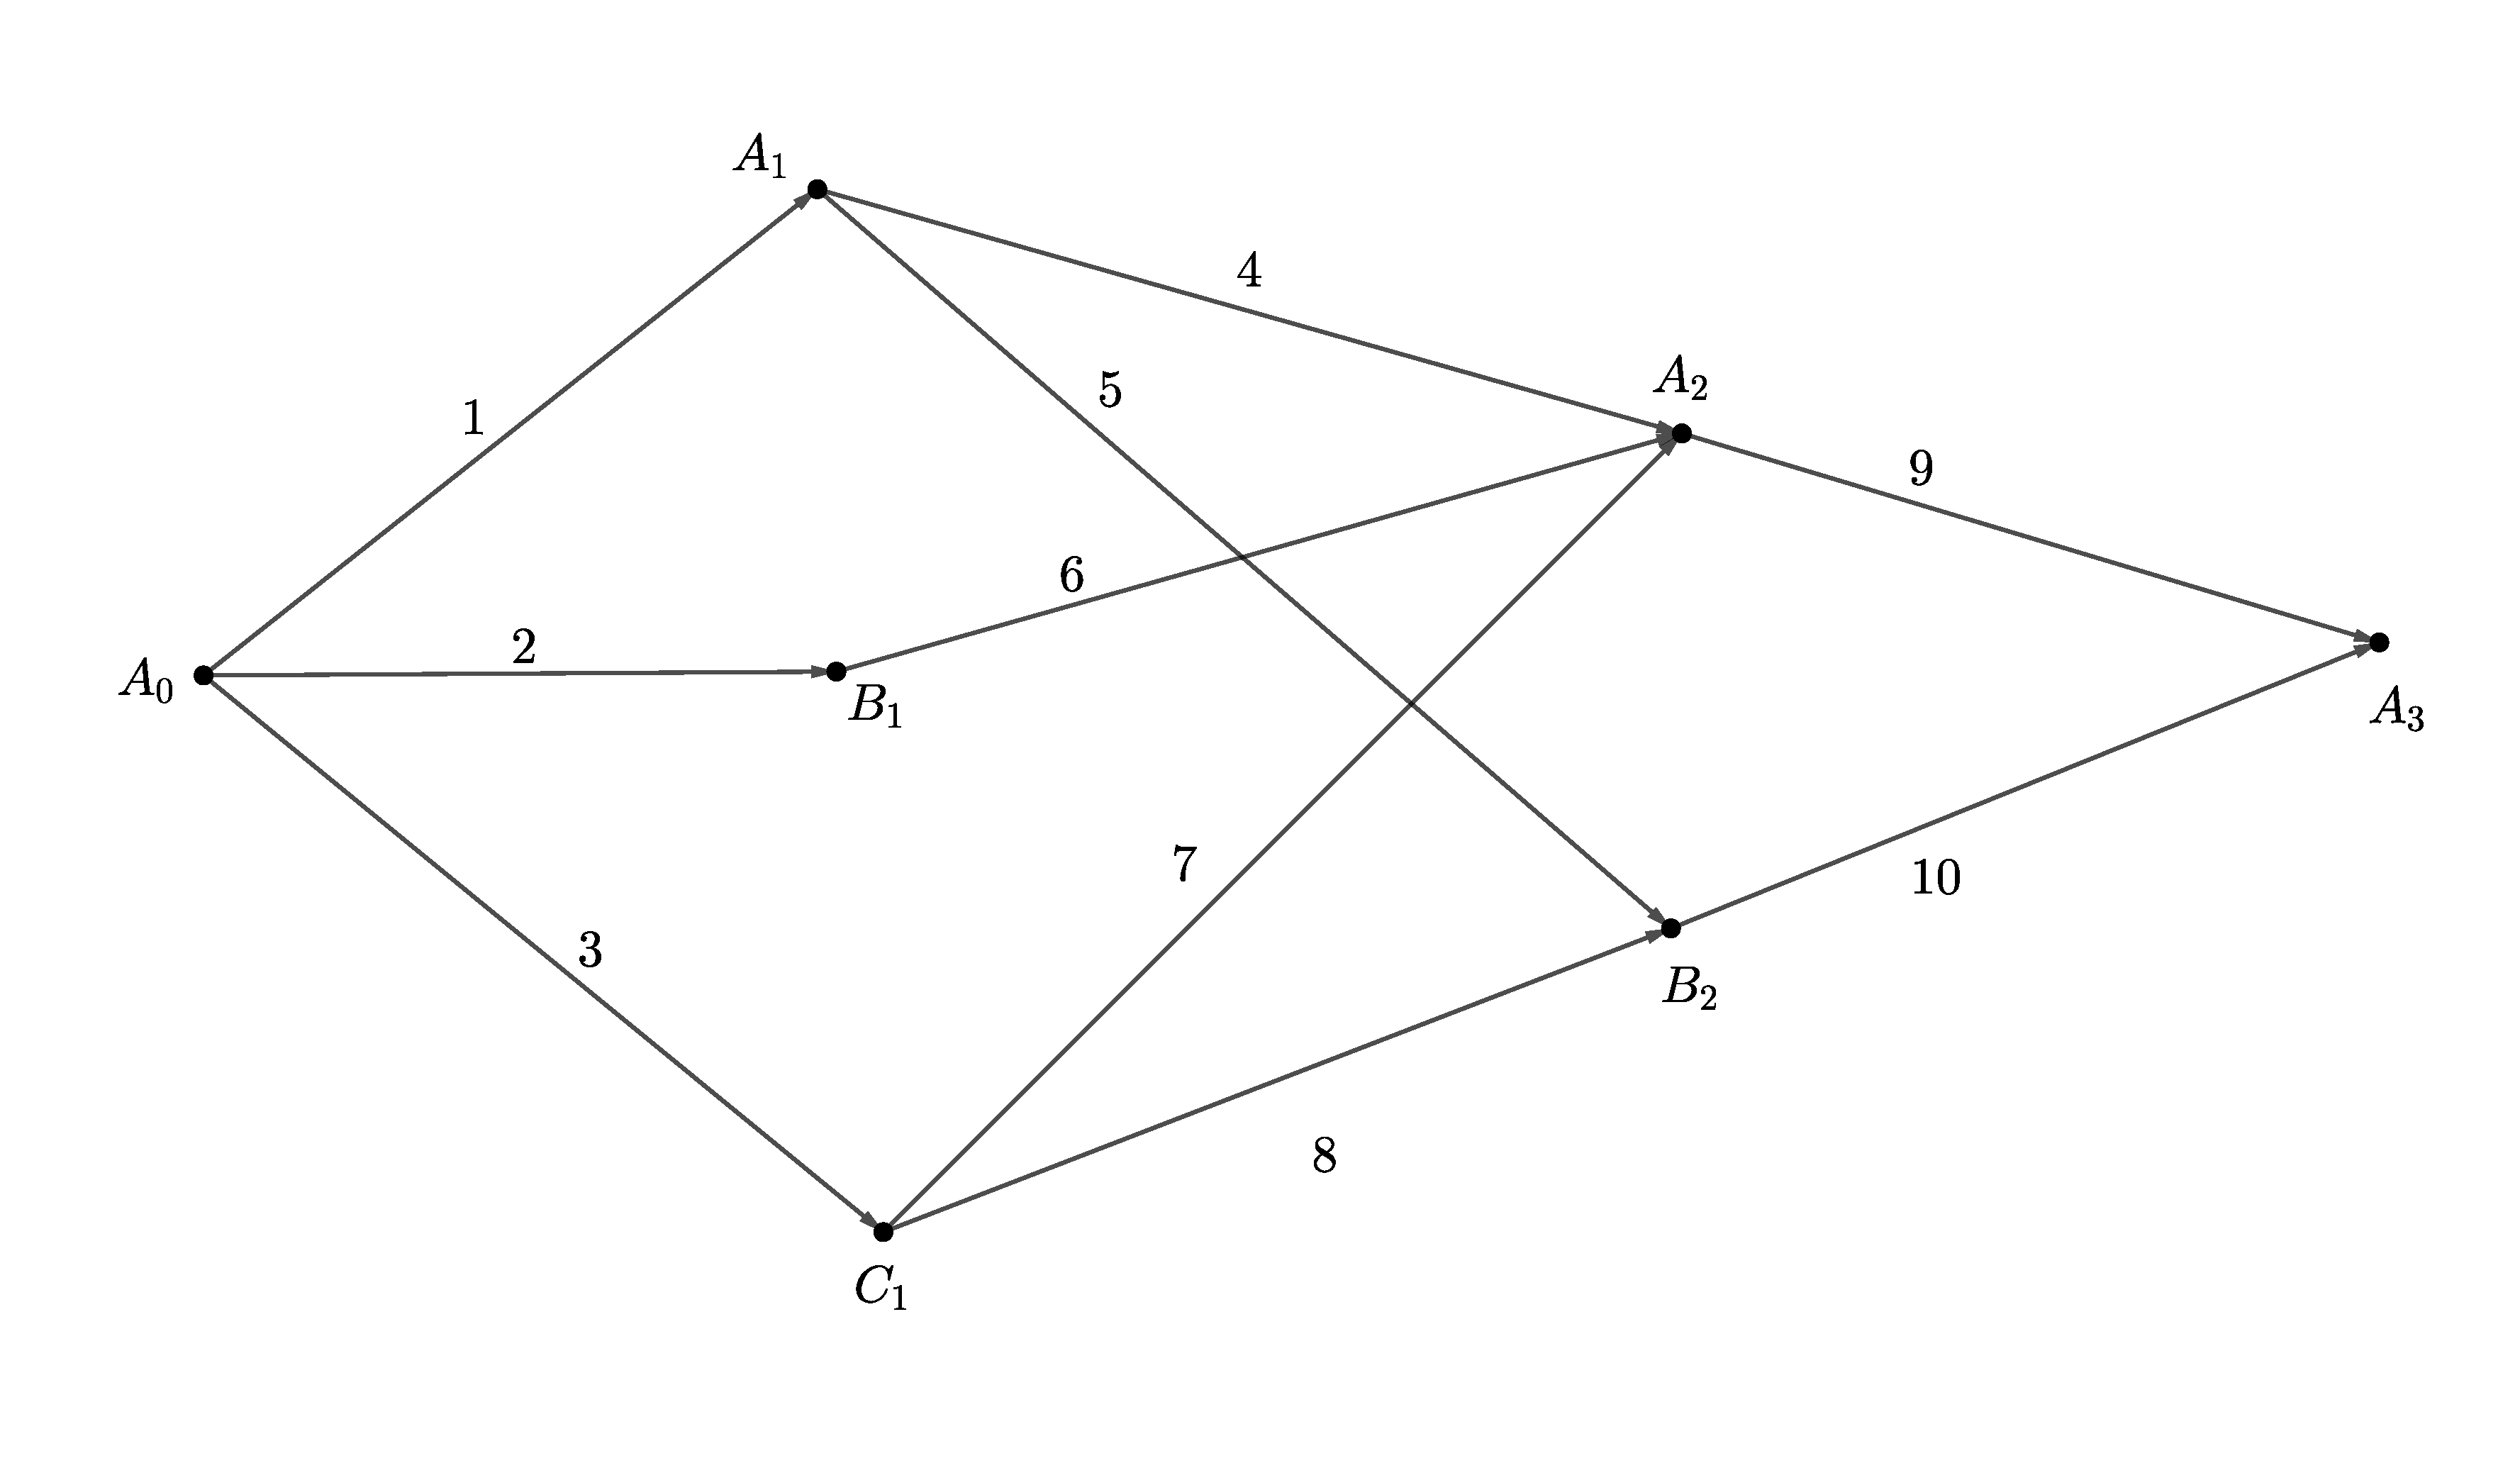
\includegraphics[scale = 0.15]{../图/最短路径}
		\caption{最短路径问题}
	\end{figure}
\end{example}

\begin{solution}
	记$f(P)$为点$P$到目标点$A_3$的最短路径长度,
	$x(P)$为点$P$在最短路径中的下一点,
	$d(P,Q)$为点$P$到点$Q$的距离。
	我们从目标点往前向出发点递推。
	
	还有$1$步到达目标点:
	\begin{align*}
		& f(A_2)=d(A_2,A_3)=9,\qquad x(A_2)=A_3\\
		& f(B_2)=d(B_2,A_3)=10,\qquad x(B_2)=A_3
	\end{align*}

	还有$2$步到达目标点:
	\begin{align*}
		& f(A_1)
		=\min\{ d(A_1,A_2)+f(A_2),d(A_1,B_2)+f(B_2) \}
		=\min\{ 13,15 \}=13,
		 && x(A_1)=A_2\\
		& f(B_1)
		=d(B_1,A_2)+f(A_2)
		=15, && x(B_1)=A_2\\
		& f(C_1)
		=\min\{ d(C_1,A_2)+f(A_2),d(C_1,B_2)+f(B_2) \}
		=\min\{ 16,18 \}
		=16, && x(C_1)=A_2
	\end{align*}
	
	还有$3$步到达目标点:%
	\begin{align*}
		&f(A_0)
		=\min\{ d(A_0,A_1)+f(A_1),d(A_0,B_1)+f(B_1),d(A_0,C_1)+f(C_1) \}
		=\min\{ 14,17,19 \}
		=14\\
		& x(A_0)=A_1
	\end{align*}
	
	所以最短路径为%
	$$
	A_0\to A_1\to A_2\to A_3,\qquad \text{min}=14
	$$
\end{solution}

\subsection{旅行售货员问题}

\begin{example}
	求解从点$v_1$出发,经过点$v_2,v_3,v_4$各一次,最后回到点$v_1$的最短路径。距离矩阵如下,其中$(i,j)$为点$v_i$到点$v_j$的距离。%
	$$
	\bs{D}=\begin{pmatrix}
		0 & 8 & 5 & 6\\
		6 & 0 & 8 & 5\\
		7 & 9 & 0 & 5\\
		9 & 7 & 8 & 0
	\end{pmatrix}
	$$
\end{example}

\begin{solution}
	记$f(v_i,V)$为从点$v_i$,经过集合$V$中的点各一次,最后回到初始点$v_1$的最短路径长度,
	$x(v_i)$为点$v_i$在最短路径中的下一点,
	$d(v_i,v_j)$为点$v_i$到点$v_j$的距离。我们从目标点往前向出发点递推。
	
	经过$0$个点,回到$v_1$:
	\begin{align*}
		& f(v_2,\varnothing)=d(v_2,v_1)=6\\
		& f(v_3,\varnothing)=d(v_3,v_1)=7\\
		& f(v_4,\varnothing)=d(v_4,v_1)=9
	\end{align*}

	经过$1$个点,回到$v_1$:
	\begin{align*}
		& f(v_2,\{ v_3 \})=d(v_2,v_3)+f(v_3,\varnothing)=15\\
		& f(v_2,\{ v_4 \})=d(v_2,v_4)+f(v_4,\varnothing)=14\\
		& f(v_3,\{ v_2 \})=d(v_3,v_2)+f(v_2,\varnothing)=15\\
		& f(v_3,\{ v_4 \})=d(v_3,v_4)+f(v_4,\varnothing)=14\\
		& f(v_4,\{ v_2 \})=d(v_4,v_2)+f(v_2,\varnothing)=13\\
		& f(v_4,\{ v_3 \})=d(v_4,v_3)+f(v_3,\varnothing)=15
	\end{align*}

	经过$2$个点,回到$v_1$:
	\begin{align*}
		& f(v_2,\{ v_3,v_4 \})
		=\min\{ d(v_2,v_3)+f(v_3,\{ v_4 \}),d(v_2,v_4)+f(v_4,\{ v_3 \}) \}
		=\min\{ 22,20 \}=20,\qquad x(v_2)=v_4\\
		& f(v_3,\{ v_2,v_4 \})
		=\min\{ d(v_3,v_2)+f(v_2,\{ v_4 \}),d(v_3,v_4)+f(v_4,\{ v_2 \}) \}
		=\min\{ 23,18 \}=18,\qquad x(v_3)=v_4\\
		& f(v_4,\{ v_2,v_3 \})
		=\min\{ d(v_4,v_2)+f(v_2,\{ v_3 \}),d(v_4,v_3)+f(v_3,\{ v_2 \}) \}
		=\min\{ 22,23 \}=22,\qquad x(v_4)=v_2
	\end{align*}

	经过$3$个点,回到$v_1$:
	\begin{align*}
		& f(v_1,\{ v_2,v_3,v_4 \})\\
		=&\min\{ d(v_1,v_2)+f(v_2,\{ v_3,v_4 \}),d(v_1,v_3)+f(v_3,\{ v_2,v_4 \}),d(v_1,v_4)+f(v_4,\{ v_2,v_3 \}) \}\\
		=&\min\{ 28,23,28 \}=23\\
		& x(v_1)=v_3
	\end{align*}
	
	所以最短路径为%
	$$
	v_1\to v_3\to v_4\to v_2\to v_1,\qquad \text{min} = 23
	$$
\end{solution}

\subsection{多阶段资源分配问题}

\begin{lemma}
	如果$g(y),h(y)$为凸函数,那么对于任意$x$,$F(y)=g(y)+h(x-y)$为凸函数。
\end{lemma}

\begin{lemma}
	如果$f(x),g(x)$为凸函数,那么$\max\{f(x),g(x)\}$为凸函数。
\end{lemma}

\begin{theorem}{多阶段资源分配问题}
	多阶段资源分配问题递推公式为%
	$$
	\begin{cases}
		\dis f_1(x)=\max_{0\le y \le x}\{ g(y)+h(x-y) \}\\
		\dis f_{k+1}(x)=\max_{0\le y \le x}\{ g(y)+h(x-y)+f_{k}(ay+b(x-y)) \}
	\end{cases}
	$$
\end{theorem}

\begin{theorem}{多阶段资源分配问题的凸函数解}
	如果$g(y)$和$h(y)$为凸函数,且$g(0)=h(0)=0$,那么$n$阶段资源分配问题的最优策略$y$在每个阶段总取$0\le y \le x$的端点的值,且%
	$$
	\begin{cases}
		f_1(x)=\max\{ g(x),h(x) \}\\
		f_{k+1}(x)=\max\{ g(x)+f_k(ax),h(x)+f_k(bx) \}
	\end{cases}
	$$
\end{theorem}

\begin{example}
	某单位有资源$100$单位,拟分$4$个周期使用,在每个周期有生产任务$A$和$B$,把资源用于$A$生产任务,每单位能获利$10$元,资源回收率为$2/3$;把资源用于$B$生产任务,每单位能获利$7$元,资源回收率为$9/10$​。问每个周期应如何分配资源,使总收益最大?
\end{example}

\begin{solution}
	记$A$生产任务的获利函数为$g(x)=10x$,$B$生产任务的获利函数为$h(x)=7x$,以及$a=2/3$,$b=9/10$。
	
	以$f_1(x)$表示投入$x$单位的生产资源在$1$个周期内生产的最大总收益函数,那么
	$$
	f_1(x)
	=\max_{0\le y \le x}\{ g(y)+h(x-y) \}
	=\max_{0\le y \le x}\{ 7x+3y \}
	=10x,\qquad y=x
	$$
	以$f_2(x)$表示投入$x$单位的生产资源在$2$个周期内生产的最大总收益函数,那么
	$$
	f_{2}(x)
	=\max_{0\le y \le x}\{ g(y)+h(x-y)+f_{1}(ay+b(x-y)) \}
	=\max_{0\le y \le x}\left\{16x+\frac{2}{3}y\right\}
	=\frac{50}{3}x,\qquad y=x
	$$
	以$f_3(x)$表示投入$x$单位的生产资源在$3$个周期内生产的最大总收益函数,那么
	$$
	f_{3}(x)
	=\max_{0\le y \le x}\{ g(y)+h(x-y)+f_{2}(ay+b(x-y)) \}
	=\max_{0\le y \le x}\left\{22 x-\frac{8 y}{9}\right\}
	=22x,\qquad y=0
	$$
	以$f_4(x)$表示投入$x$单位的生产资源在$4$个周期内生产的最大总收益函数,那么
	$$
	f_{4}(x)
	=\max_{0\le y \le x}\{ g(y)+h(x-y)+f_{3}(ay+b(x-y)) \}
	=\max_{0\le y \le x}\left\{\frac{134}{5}x-\frac{32}{15}y\right\}
	=\frac{134}{5}x,\quad y=0
	$$
	因此投入$100$单位的生产资源在$4$个周期内生产的最大总收益为
	$$
	f_4(100)=2680
	$$
	
	每个阶段的生产计划如下
	\begin{table}[H]
		\centering
		\caption{生产计划}
		\begin{tabular}{c|ccc}
			\hline
			 & 投入$A$生产任务 & 投入$B$生产任务 & 本周期收益 \\ \hline
			第一周期 & $0$ & $100$ & $700$ \\
			第二周期 & $0$ & $90$ & $630$ \\
			第三周期 & $81$ & $0$ & $810$ \\
			第四周期 & $54$ & $0$ & $540$ \\ \hline
			总收益 & & & $2680$ \\ \hline
		\end{tabular}
	\end{table}
\end{solution}

\subsection{可靠性问题}

\begin{example}
	求解规划问题
	\begin{align*}
		& \text{max}  \quad z=x_1x_2\cdots x_n\\
		& \text{s.t.} \;\, \quad \begin{cases}
			x_1+x_2+\cdots+x_n=1\\
			x_1,x_2,\cdots,x_n\ge 0
		\end{cases}
	\end{align*}
\end{example}

\begin{solution}
	令%
	$$
	f_k(x)=\max\{ x_1x_2\cdots x_k:x_1+x_2+\cdots+x_k=1,x_1,x_2,\cdots,x_k\ge 0 \}
	$$
	那么成立递推关%
	$$
	\begin{cases}
		f_1(x)=x\\
		\dis f_{k+1}(x)=\max_{0\le x_{k+1}\le x}x_{k+1}f_{k}(x-x_k)
	\end{cases}
	$$
	从而%
	$$
	f_k(x)=\max_{0\le x_k \le x}x_k\left(\frac{x-x_k}{k-1}\right)^{n-1}=\frac{x^k}{k^k},\qquad x_k=\frac{x}{k}
	$$
	
	现在来求最优解。
	
	第一阶段,状态变量$x=1$,最优解$x_n=\frac{1}{n}$。
	
	第二阶段,状态变量%
	$$
	x=1-\frac{1}{n}=\frac{n-1}{n}
	$$
	最优解%
	$$
	x_{n-1}=\frac{x}{n-1}=\frac{1}{n}
	$$
	
	第三阶段,状态变量%
	$$
	x=1-\frac{1}{n}-\frac{1}{n}=\frac{n-2}{n}
	$$
	最优解%
	$$
	x_{n-2}=\frac{x}{n-2}=\frac{1}{n}
	$$
	
	以此类推,最后阶段,状态变量%
	$$
	x=1-\frac{1}{n}-\frac{1}{n}-\cdots-\frac{1}{n}=\frac{1}{n}
	$$
	最优解%
	$$
	x_{n-2}=\frac{x}{1}=\frac{1}{n}
	$$
	
	进而最优解为$\left(\frac{1}{n},\frac{1}{n},\cdots,\frac{1}{n}\right)$,最优值为$1/n^n$。
\end{solution}

\begin{example}
	求解规划问题
	\begin{align*}
		& \text{max}  \quad z=4x_1^2-x_2^2+2x_3^2+12\\
		& \text{s.t.} \;\, \quad \begin{cases}
			3x_1+2x_2+x_9\\
			x_1,x_2,x_3\ge 0
		\end{cases}
	\end{align*}
\end{example}

\begin{solution}
	第一阶段%
	$$
	f_1(y)=\max_{0\le 3 x_1\le y}\{ 4x_1^2 \}=\frac{4}{9}y^2,\qquad x_1=\frac{y}{3}
	$$
	第二阶段%
	$$
	f_2(y)=\max_{0\le 2x_2\le y}\{ -x_2^2+f_1(y-2x_2) \}
	=\frac{4}{9}y^2,\qquad x_2=0
	$$
	第三阶段%
	$$
	f_3(9)=\max_{0\le x_3\le 9}\{ 2x_3^2+12+f_2(9-x_3) \}
	=174,\qquad x_3=9
	$$
	因此最优解为%
	$$
	x_1=0,\qquad
	x_2=0,\qquad
	x_3=9
	$$
\end{solution}

\section{确定性的不定期多阶段决策问题}

\subsection{最优线路问题}

\begin{definition}{最优线路问题}
	\begin{equation}\label{最优线路问题}
		\begin{cases}
			f(i)=\min\limits_{1\le j \le n}\{ c_{ij}+f(j) \},\qquad i=1,2,\cdots,n-1\\
			f(n)=0
		\end{cases}\tag{*}
	\end{equation}
\end{definition}

\begin{theorem}{函数空间迭代法}
	记$f_k(i)$为由$v_i$点出发至多经过$k$个点到达$v_n$的最短路程,那么%
	$$
	\begin{cases}
		f_1(i)=c_{in},\qquad i=1,2,\cdots,n-1\\
		f_1(n)=0
	\end{cases}
	$$
	递推关系为%
	$$
	\begin{cases}
		f_k(i)=\min\limits_{1\le j \le n}\{ c_{ij}+f_{k-1}(j) \},\qquad i=1,2,\cdots,n-1\\
		f_k(n)=0
	\end{cases}
	$$
	得到的函数列$\{ f_k(i) \}$单调下降收敛于函数方程(\ref{最优线路问题})的解$f(i)$。
\end{theorem}

\begin{example}
	设有五个城市$1,2,3,4,5$相互的距离矩阵为
	$$
	\boldsymbol{D}=\begin{pmatrix}
		0 & 3 & 4 & \infty & \infty \\
		\infty & 0 & 5 & 2 & 4 \\
		\infty & \infty & 0 & 3 & \infty \\
		\infty & \infty & \infty & 0 & 1 \\
		\infty & \infty & \infty & \infty & 0 \\
	\end{pmatrix}
	$$
	试用函数空间迭代法求各城市到城市$5$的最短路线及最短路程。
\end{example}

\begin{solution}
	记$f_1(i)$为由城市$i$出发至多经过$1$个城市到达城市$5$的最短路程,那么
	$$
	\small{
		f_1(1)=d_{15}=\infty,\quad 
		f_1(2)=d_{25}=4,\quad
		f_1(3)=d_{35}=\infty,\quad
		f_1(4)=d_{45}=1,\quad
		f_1(5)=d_{55}=0
	}
	$$
	
	记$f_2(i)$为由城市$i$出发至多经过$2$个城市到达城市$5$的最短路程,那么
	\begin{align*}
		& f_2(1)
		=\min_{1\le j \le 5}\{ d_{1j}+f_1(j) \}
		=\min\{ 0+\infty, 3+4, 4+\infty, \infty+1, \infty+0 \}
		=7\\
		& f_2(2)
		=\min_{1\le j \le 5}\{ d_{2j}+f_1(j) \}
		=\min\{ \infty+\infty, 0+4, 5+\infty, 2+1, 4+0 \}
		=3\\
		& f_2(3)=\min_{1\le j \le 5}\{ d_{3j}+f_1(j) \}
		=\min\{ \infty+\infty, \infty+4, 0+\infty, 3+1, \infty+0 \}
		=4\\
		& f_2(4)=\min_{1\le j \le 5}\{ d_{4j}+f_1(j) \}
		=\min\{ \infty+\infty, \infty+4, \infty+\infty, 0+1, 1+0 \}
		=1\\
		& f_2(5)=0
	\end{align*}
	
	记$f_3(i)$为由城市$i$出发至多经过$3$个城市到达城市$5$的最短路程,那么
	\begin{align*}
		& f_3(1)
		=\min_{1\le j \le 5}\{ d_{1j}+f_2(j) \}
		=\min\{ 0+7, 3+3, 4+4, \infty+1, \infty+0 \}
		=6\\
		& f_3(2)
		=\min_{1\le j \le 5}\{ d_{2j}+f_2(j) \}
		=\min\{ \infty+7, 0+3, 5+4, 2+1, 4+0 \}
		=3\\
		& f_3(3)
		=\min_{1\le j \le 5}\{ d_{3j}+f_2(j) \}
		=\min\{ \infty+7, \infty+3, 0+4, 3+1, \infty+0 \}
		=4\\
		& f_3(4)
		=\min_{1\le j \le 5}\{ d_{4j}+f_2(j) \}
		=\min\{ \infty+7, \infty+3, \infty+4, 0+1, 1+0 \}
		=1\\
		& f_3(5)=0
	\end{align*}
	
	记$f_4(i)$为由城市$i$出发至多经过$4$个城市到达城市$5$的最短路程,那么
	\begin{align*}
		& f_4(1)
		=\min_{1\le j \le 5}\{ d_{1j}+f_3(j) \}
		=\min\{ 0+6, 3+3, 4+4, \infty+1, \infty+0 \}
		=6,&&
		s(1)=2\\
		& f_4(2)
		=\min_{1\le j \le 5}\{ d_{2j}+f_3(j) \}
		=\min\{ \infty+6, 0+3, 5+4, 2+1, 4+0 \}
		=3,&&
		s(2)=4\\
		& f_4(3)
		=\min_{1\le j \le 5}\{ d_{3j}+f_3(j) \}
		=\min\{ \infty+6, \infty+3, 0+4, 3+1, \infty+0 \}
		=4,&&s(3)=4\\
		& f_4(4)
		=\min_{1\le j \le 5}\{ d_{4j}+f_3(j) \}
		=\min\{ \infty+6, \infty+3, \infty+4, 0+1, 1+0 \}
		=1,&&
		s(4)=5\\
		& f_4(5)=0
	\end{align*}
	
	因此各城市到城市$5$的最短路线及最短路程为
	\begin{table}[H]
		\centering
		\begin{tabular}{ccc}
			\toprule
			\textbf{城市} & \textbf{最短路线} & \textbf{最短路程} \\
			\midrule
			$1$ & $1\to 2\to 4\to 5$ & $6$ \\
			$2$ & $2\to 4 \to 5$ & $3$ \\
			$3$ & $3\to 4\to 5$ & $4$ \\
			$4$ & $4\to 5$ & $1$ \\
			\bottomrule
		\end{tabular}
	\end{table}
\end{solution}

\begin{theorem}{策略空间迭代法}
	策略$\{ s(i) \}$就是给定在点$v_i$时,选定下一步的位置为$s(i)$。
	
	给定无回路的初始策略$\{ s_0(i) \}$,作方程组%
	$$
	\begin{cases}
		f_0(i)=c_{i,s_0(i)}+f_0(s_0(i)),\qquad i=1,2,\cdots,n-1\\
		f_0(n)=0
	\end{cases}
	$$
	解得$f_0(1),\cdots,f_0(n)$。求解%
	$$
	\min_{1\le  j \le n}\{ c_{ij}+f_0(j) \}=c_{i,s_1(i)}+f_0(s_1(i)),\qquad i=1,2,\cdots,n-1
	$$
	由此得到策列$\{ s_1(i) \}$。重复上面过程,得到策略$\{ s_k(i) \}$,由此得到的函数列$\{ f_k(i) \}$单调下降收敛于函数方程(\ref{最优线路问题})的解$f(i)$。
\end{theorem}

\begin{example}
	设有五个城市$1,2,3,4,5$相互的距离矩阵为
	$$
	\boldsymbol{D}=\begin{pmatrix}
		0 & 3 & 4 & \infty & \infty \\
		\infty & 0 & 5 & 2 & 4 \\
		\infty & \infty & 0 & 3 & \infty \\
		\infty & \infty & \infty & 0 & 1 \\
		\infty & \infty & \infty & \infty & 0 \\
	\end{pmatrix}
	$$
	试用策略空间迭代法求各城市到城市$5$的最短路线及最短路程,其中初始策略为%
	$$
	s_0(1)=2,\qquad
	s_0(2)=3,\qquad
	s_0(3)=4,\qquad
	s_0(4)=5,\qquad
	s_0(5)=5
	$$
\end{example}

\begin{solution}
	作方程组
	$$
	\begin{cases}
		f_0(1)=d_{1,s_0(1)}+f_0(s_0(1))\\
		f_0(2)=d_{2,s_0(2)}+f_0(s_0(2))\\
		f_0(3)=d_{3,s_0(3)}+f_0(s_0(3))\\
		f_0(4)=d_{4,s_0(4)}+f_0(s_0(4))\\
		f_0(5)=0
	\end{cases}
	\iff
	\begin{cases}
		f_0(1)=3+f_0(2)\\
		f_0(2)=5+f_0(3)\\
		f_0(3)=3+f_0(4)\\
		f_0(4)=1+f_0(5)\\
		f_0(5)=0
	\end{cases}
	\iff
	\begin{cases}
		f_0(1)=12\\
		f_0(2)=9\\
		f_0(3)=4\\
		f_0(4)=1\\
		f_0(5)=0
	\end{cases}
	$$
	求解
	\begin{align*}
		& \min_{1\le  j \le 5}\{ d_{1j}+f_0(j) \}
		=\min\{ 0+12, 3+9, 4+4, \infty+1, \infty+0 \}
		=8,&&
		s_1(1)=3\\
		& \min_{1\le  j \le 5}\{ d_{2j}+f_0(j) \}
		=\min\{ \infty+12, 0+9, 5+4, 2+1, 4+0 \}
		=3,&&
		s_1(2)=4\\
		& \min_{1\le  j \le 5}\{ d_{3j}+f_0(j) \}
		=\min\{ \infty+12, \infty+9, 0+4, 3+1, \infty+0 \}
		=4,&&
		s_1(3)=4\\
		& \min_{1\le  j \le 5}\{ d_{4j}+f_0(j) \}
		=\min\{ \infty+12, \infty+9, \infty+4, 0+1, 1+0 \}
		=1,&&
		s_1(4)=5
	\end{align*}
	由此得到策略
	$$
	s_1(1)=3,\qquad
	s_1(2)=4,\qquad
	s_1(3)=4,\qquad
	s_1(4)=5,\qquad
	s_1(5)=5
	$$
	
	作方程组
	$$
	\begin{cases}
		f_1(1)=d_{1,s_1(1)}+f_1(s_1(1))\\
		f_1(2)=d_{2,s_1(2)}+f_1(s_1(2))\\
		f_1(3)=d_{3,s_1(3)}+f_1(s_1(3))\\
		f_1(4)=d_{4,s_1(4)}+f_1(s_1(4))\\
		f_1(5)=0
	\end{cases}
	\iff
	\begin{cases}
		f_1(1)=4+f_1(3)\\
		f_1(2)=2+f_1(4)\\
		f_1(3)=3+f_1(4)\\
		f_1(4)=1+f_1(5)\\
		f_1(5)=0
	\end{cases}
	\iff
	\begin{cases}
		f_1(1)=8\\
		f_1(2)=3\\
		f_1(3)=4\\
		f_1(4)=1\\
		f_1(5)=0
	\end{cases}
	$$
	求解
	\begin{align*}
		& \min_{1\le  j \le 5}\{ d_{1j}+f_1(j) \}
		=\min\{ 0+8, 3+3, 4+4, \infty+1, \infty+0 \}
		=6,&&
		s_2(1)=2\\
		& \min_{1\le  j \le 5}\{ d_{2j}+f_1(j) \}
		=\min\{ \infty+8, 0+3, 5+4, 2+1, 4+0 \}
		=3,&&
		s_2(2)=4\\
		& \min_{1\le  j \le 5}\{ d_{3j}+f_1(j) \}
		=\min\{ \infty+8, \infty+3, 0+4, 3+1, \infty+0 \}
		=4,&&
		s_2(3)=4\\
		& \min_{1\le  j \le 5}\{ d_{4j}+f_1(j) \}
		=\min\{ \infty+8, \infty+3, \infty+4, 0+1, 1+0 \}
		=1,&&
		s_2(4)=5
	\end{align*}
	由此得到策略
	$$
	s_2(1)=2,\qquad
	s_2(2)=4,\qquad
	s_2(3)=4,\qquad
	s_2(4)=5,\qquad
	s_2(5)=5
	$$
	
	作方程组
	$$
	\begin{cases}
		f_2(1)=d_{1,s_2(1)}+f_1(s_2(1))\\
		f_2(2)=d_{2,s_2(2)}+f_1(s_2(2))\\
		f_2(3)=d_{3,s_2(3)}+f_1(s_2(3))\\
		f_2(4)=d_{4,s_2(4)}+f_1(s_2(4))\\
		f_2(5)=0
	\end{cases}
	\iff
	\begin{cases}
		f_2(1)=3+f_1(2)\\
		f_2(2)=2+f_1(4)\\
		f_2(3)=3+f_1(4)\\
		f_2(4)=1+f_1(5)\\
		f_2(5)=0
	\end{cases}
	\iff
	\begin{cases}
		f_2(1)=6\\
		f_2(2)=3\\
		f_2(3)=4\\
		f_2(4)=1\\
		f_2(5)=0
	\end{cases}
	$$
	求解
	\begin{align*}
		& \min_{1\le  j \le 5}\{ d_{1j}+f_2(j) \}
		=\min\{ 0+6, 3+3, 4+4, \infty+1, \infty+0 \}
		=6,&&
		s_3(1)=2\\
		& \min_{1\le  j \le 5}\{ d_{2j}+f_2(j) \}
		=\min\{ \infty+6, 0+3, 5+4, 2+1, 4+0 \}
		=3,&&
		s_3(2)=4\\
		& \min_{1\le  j \le 5}\{ d_{3j}+f_2(j) \}
		=\min\{ \infty+6, \infty+3, 0+4, 3+1, \infty+0 \}
		=4,&&
		s_3(3)=4\\
		& \min_{1\le  j \le 5}\{ d_{4j}+f_2(j) \}
		=\min\{ \infty+6, \infty+3, \infty+4, 0+1, 1+0 \}
		=1,&&
		s_3(4)=5
	\end{align*}
	由此得到策略
	$$
	s_3(1)=2,\qquad
	s_3(2)=4,\qquad
	s_3(3)=4,\qquad
	s_3(4)=5,\qquad
	s_3(5)=5
	$$
	
	因此各城市到城市$5$的最短路线及最短路程为
	\begin{table}[H]
		\centering
		\begin{tabular}{ccc}
			\toprule
			\textbf{城市} & \textbf{最短路线} & \textbf{最短路程} \\
			\midrule
			$1$ & $1\to 2\to 4\to 5$ & $6$ \\
			$2$ & $2\to 4 \to 5$ & $3$ \\
			$3$ & $3\to 4\to 5$ & $4$ \\
			$4$ & $4\to 5$ & $1$ \\
			\bottomrule
		\end{tabular}
	\end{table}
\end{solution}

\chapter{图与网络分析}

\section{图的基本概念与矩阵表示}

\subsection{图的基本概念}

\begin{definition}{图}
	\begin{enumerate}
		\item 称二元组$(V,E)$为无向图,其中$V$为点集合
		$$
		E=\{ \langle u,v \rangle\text{为无序偶}  \}
		$$
		为无向边集合。
		\item 称二元组$(V,E)$为有向图,其中$V$为点集合
		$$
		E=\{ (u,v)\text{为有序偶}  \}
		$$
		为有向边集合。
	\end{enumerate}
\end{definition}

\begin{definition}{点与边的关系}
	\begin{enumerate}
		\item 点与边的关联
		\begin{enumerate}
			\item 称无向边$\langle u,v \rangle$与点$u,v$关联。
			\item 称有向边$(u,v)$与点$u,v$关联。
		\end{enumerate}
		\item 点与点的邻接
		\begin{enumerate}
			\item 称点$u,v$邻接,如果存在无向边$\langle u,v \rangle$。
			\item 称点$u,v$邻接,如果存在有向边$(u,v)$。
		\end{enumerate}
		\item 边与边的邻接
		\begin{enumerate}
			\item 称无向边$\langle u,v \rangle$与$\langle x,y \rangle$邻接,如果$\{ u,v \}\cap\{ x,y \}\ne\varnothing$。
			\item 称有向边$(u,v)$与$(x,y)$邻接,如果$\{ u,v \}\cap\{ x,y \}\ne\varnothing$。
		\end{enumerate}
	\end{enumerate}
\end{definition}

\begin{definition}{特殊点}
	\begin{enumerate}
		\item 端点:称点$u,v$为无向边$\langle u,v \rangle$的端点。
		\item 起点/尾:称点$u$为有向边$(u,v)$的起点/尾。
		\item 终点/头:称点$v$为有向边$(u,v)$的终点/头。
		\item 孤立点
		\begin{enumerate}
			\item 称点$v$为孤立点,如果不存在无向边$\langle u,w \rangle$,使得$v\in\{ u,w \}$。
			\item 称点$v$为孤立点,如果不存在有向边$(u,w)$,使得$v\in\{ u,w \}$。
		\end{enumerate}
	\end{enumerate}
\end{definition}

\begin{definition}{特殊边}
	\begin{enumerate}
		\item 环
		\begin{enumerate}
			\item 称无向边$\langle v,v \rangle$为环。
			\item 称有向边$(v,v)$为环。
		\end{enumerate}
		\item 重边
		\begin{enumerate}
			\item 称无向边$\langle u,v \rangle$与$\langle u,v \rangle$为重边。
			\item 称有向边$(v,v)$与$(v,v)$为重边。
		\end{enumerate}
	\end{enumerate}
\end{definition}

\begin{definition}{特殊图}
	\begin{enumerate}
		\item 简单图:称图为简单图,如果其既没有环,也没有重边。
		\item 完全图
		\begin{enumerate}
			\item 称简单无向图$(V,E)$为完全无向图$K_n$,其中$|V|=n$,如果对于任意$u,v\in V$,成立$\langle u,v \rangle\in E$。
			\item 称简单有向图$(V,E)$为完全有向图$K_n$,其中$|V|=n$,如果对于任意$u,v\in V$,成立$(u,v)\in E$且$(v,u)\in E$。
		\end{enumerate}
		\item 二分图
		\begin{enumerate}
			\item 称无向图$(V,E)$为二分无向图,并记作$(S,T,E)$,如果$V=S\sqcup T$,且对于任意$\langle s,t \rangle\in E$,成立$s\in S$与$t\in T$。
			\item 称有向图$(V,E)$为二分无向图,并记作$(S,T,E)$,如果$V=S\sqcup T$,且对于任意$(s,t)\in E$,成立$s\in S$与$t\in T$。
		\end{enumerate}
		\item 完全二分图
		\begin{enumerate}
			\item 称简单二分无向图$(S,T,E)$为完全二分无向图$K_{p,q}$,其中$|S|=p$且$|T|=q$,如果对于任意$s\in S$与$t\in T$,存在$\langle s,t \rangle\in E$。
			\item 称简单二分有向图$(S,T,E)$为完全二分有向图$K_{p,q}$,其中$|S|=p$且$|T|=q$,如果对于任意$s\in S$与$t\in T$,存在$(s,t)\in E$。
		\end{enumerate}
		\item 补图:对于简单图$G=(V,E)$,令$K_n=(V,E_K)$为完全图,定义$G$的补图为$\overline{G}=(V,E_K\setminus E)$。
		\item 基本图:称无向图$(V,E_0)$为有向图$(V,E)$的基本图,如果成立如下命题。
		\begin{enumerate}
			\item 对于任意$(u,v)\in E$,成立$\langle u,v \rangle\in E_0$。
			\item 对于任意$\langle u,v \rangle\in E_0$,成立$(u,v)\in E$。
		\end{enumerate}
	\end{enumerate}
\end{definition}

\begin{definition}{图依大小的分类}
	\begin{enumerate}
		\item 有限图:称图$(V,E)$为有限图,如果$|V|<\infty$且$|E|<\infty$。
		\item 无限图:称图$(V,E)$为无限图,如$|V|=\infty$或$|E|=\infty$。
		\item 空图:称图$(V,E)$为空图,如果$V=\varnothing$。
		\item 平凡图:称图$(V,E)$为平凡图,如果$|V|=1$。
	\end{enumerate}
\end{definition}

\begin{definition}{网络}
	对于图$(V,E)$,定义$(V,E,\varphi)$为网络,其中$\varphi:E\to\R$为函数。
\end{definition}

\begin{definition}{图的运算}
	\begin{enumerate}
		\item 并:定义图$G_1=(N_1,E_1)$与$G_2=(N_2,E_2)$的并为图%
		$$
		G_1\cup G_2=\left(N_1\cup N_2,E_1\cup N_2\right)
		$$
		\item 交:定义图$G_1=(N_1,E_1)$与$G_2=(N_2,E_2)$的交为图%
		$$
		G_1\cap G_2=\left(N_1\cap N_2,E_1\cap N_2\right)
		$$
		\item 不交:称图$G_1=(N_1,E_1)$与$G_2=(N_2,E_2)$不相交,如果$N_1\cap N_2=\varnothing$。
	\end{enumerate}
\end{definition}

\subsection{图的关联矩阵与邻接矩阵}

\begin{definition}{关联矩阵}
	\begin{enumerate}
		\item 定义简单无向图$(V,E)$的关联矩阵为$|V|\times |E|$阶矩阵$\bs{B}=(b_{ij})$,其中
		$$
		b_{ij}=\begin{cases}
			1,\qquad & \text{点}v_i\text{与边}e_j\text{关联}\\
			0,\qquad & \text{点}v_i\text{与边}e_j\text{不关联}
		\end{cases}
		$$
		\item 定义简单有向图$(V,E)$的关联矩阵为$|V|\times |E|$阶矩阵$\bs{B}=(b_{ij})_{|V|\times |E|}$,其中
		$$
		b_{ij}=\begin{cases}
			1,\qquad & \text{边}e_j\text{以点}v_i\text{为起点}\\
			-1,\qquad & \text{边}e_j\text{以点}v_i\text{为终点}\\
			0,\qquad & \text{其余情况}
		\end{cases}
		$$
	\end{enumerate}
\end{definition}

\begin{definition}{邻接矩阵}
	\begin{enumerate}
		\item 定义简单无向图$(V,E)$的邻接矩阵为$|V|$阶矩阵$\bs{A}=(a_{ij})$,其中
		$$
		a_{ij}=\begin{cases}
			1,\qquad & \langle v_i,v_j \rangle\in E\\
			0,\qquad & \langle v_i,v_j \rangle\notin E
		\end{cases}
		$$
		\item 定义简单有向图$(V,E)$的邻接矩阵为$|V|$阶矩阵$\bs{A}=(a_{ij})$,其中
		$$
		a_{ij}=\begin{cases}
			1,\qquad & (v_i,v_j)\in E\\
			0,\qquad & (v_i,v_j)\notin E
		\end{cases}
		$$
	\end{enumerate}
\end{definition}

\begin{definition}{度}
	\begin{enumerate}
		\item 定义简单无向图$(V,E)$的点$v$的度$\deg(v)$为图中与点$v$关联的边数;换言之%
		$$
		\deg(v)=\sum_{e\in E\text{与}v\text{关联}}1
		$$
		\item 定义简单有向图$(V,E)$的点$v$的入度$\deg^-(v)$为图中以点$v$为起点的边数;换言之%
		$$
		\deg^-(v)=\sum_{e\in E\text{以 }v\text{为起点}}1
		$$
		\item 定义简单有向图$(V,E)$的点$v$的出度$\deg^+(v)$为图中以点$v$为终点的边数;换言之%
		$$
		\deg^+(v)=\sum_{e\in E\text{以 }v\text{为终点}}1
		$$
	\end{enumerate}
\end{definition}

\begin{theorem}{二分图的等价定义}
	$G$为二分图,当且仅当$G$的邻接矩阵可表示为%
	$$
	\bs{A}=\begin{pmatrix}
		\bs{O} & \bs{M}\\
		\bs{M}^T & \bs{O}
	\end{pmatrix}
	$$
\end{theorem}

\begin{theorem}
	\begin{enumerate}
		\item 对于简单无向图$(V,E)$,成立%
		$$
		\sum_{v\in V}\deg(v)=2|E|
		$$
		\item 对于简单有向图$(V,E)$,成立
		$$
		\sum_{v\in V}\deg^+(v)=\sum_{v\in V}\deg^-(v)=|E|
		$$
	\end{enumerate}
\end{theorem}

\subsection{子图}

\begin{definition}{子图}
	\begin{enumerate}
		\item 称无向图$(V_0,E_0)$为图$(V,E)$的子图,如果$V_0\sub V$与$E_0\sub E$,且对于任意$\langle u,v \rangle\in E_0$,成立$u\in N_0$与$v\in N_0$。
		\item 称有向图$(V_0,E_0)$为图$(V,E)$的子图,如果$V_0\sub V$与$E_0\sub E$,且对于任意$(u,v)\in E_0$,成立$u\in N_0$与$v\in N_0$。
	\end{enumerate}
\end{definition}

\begin{definition}{特殊子图}
	\begin{enumerate}
		\item 支撑子图:称图$(V,E)$的子图$(V_0,E_0)$为支撑子图,如果$V_0=V$。
		\item 点导出子图:称图$G=(V,E)$的子图$G_0=(V_0,E_0)$为由点$V_0$导出的$G$的子图,并记作$G[V_0]$,如果
		$$
		E_0=\bigcup_{(V_0,E')\text{为}(V,E)\text{的子图}}E'
		$$
		\item 边导出子图:称图$G=(V,E)$的子图$G_0=(V_0,E_0)$为由边$E_0$导出的$G$的子图,并记作$G[E_0]$,如果
		$$
		V_0=\bigcup_{(V',E_0)\text{为}(V,E)\text{的子图}}V'
		$$
	\end{enumerate}
\end{definition}

\section{图的连通性}

\subsection{图的连通}

\begin{definition}{路}
	称图中从点$a$到$z$的路为点和边的交错序列
	$$
	(a,e_{ab},b,\cdots,y,e_{yz},z)
	$$
	特别的,称简单图中从点$a$到$z$的路为点的序列
	$$
	(a,b,\cdots,y,z)
	$$
\end{definition}

\begin{definition}{特殊路}
	\begin{enumerate}
		\item 简单路:称边不重复的路为简单路。
		\item 初级路:称点不重复的路为初级路。
		\item 回路:称路
		$$
		(a,e_{ab},b,\cdots,y,e_{yz},z)
		$$
		为回路,如果$a=z$。
	\end{enumerate}
\end{definition}

\begin{definition}{连通性}
	\begin{enumerate}
		\item 点的连通:对于无向图,称点$u$与$v$连通,如果存在从$u$到$v$的路。
		\item 连通图:称无向图为连通图,如果其任意两点间均连通。
		\item 连通分支:无向图的极大连通子图称为连通分支。
	\end{enumerate}
\end{definition}

\begin{definition}{强连通性}
	\begin{enumerate}
		\item 点的连通:对于有向图,称点$u$与$v$连通,如果存在从$u$到$v$的路。
		\item 强连通图:称有向图为连通图,如果其任意两点间均强连通。
		\item 强连通分支:有向图的极大强连通子图称为强连通分支。
	\end{enumerate}
\end{definition}

\subsection{图的割集}

\begin{definition}{割边}
	称图$(V,E)$的边$e$为割边,如果成立如下命题之一。
	\begin{enumerate}
		\item 子图$(N,E\setminus\{e\})$的连通分支数严格大于图$(V,E)$的连通分支数。
		\item 边$e$不包含在$G$的任意简单回路中。
	\end{enumerate}
\end{definition}

\begin{definition}{边割}
	对于图$(V,E)$,令
	$$
	\{ S,N\setminus S \}=\{ \{n_i,n_j\}\in E:n_i\in S,n_j\in N\setminus S \}
	$$
	称子集$T\sub \{ S,N\setminus S \}$为边割,如果子图$(N,E\setminus T)$的连通分支数严格大于图$(V,E)$的连通分支数。
\end{definition}

\begin{definition}{割集}
	图的极小边割称为割集。
\end{definition}

\begin{theorem}
	边割为不交割集的并。
\end{theorem}

\begin{theorem}
	对于图$G$,如果$C$为$G$的简单回路,$\Omega$为$G$的割集,令$E(C),E(\Omega)$分别表示$C,\Omega$所包含的边集合,那么或$E(C)\cap E(\Omega)=\varnothing$,或$|E(C)\cap E(\Omega)|\ge2$。
\end{theorem}

\section{树与支撑树}

\subsection{树及其基本性质}

\begin{definition}{树}
	称无向图$T=(V,E)$为树,如果成立如下命题之一。
	\begin{enumerate}
		\item 无回路且连通。
		\item 无回路且$|E|=|V|-1$。
		\item 连通且$|E|=|V|-1$。
		\item 连通且每一条边均为割边。
		\item 任意两点间存在且存在唯一一条路。
		\item 无回路,但任意增加一条新边,存在且存在唯一回路。
	\end{enumerate}
\end{definition}

\begin{proof}
	$1\implies 5$:设$T$连通且无回路,任取两点$i,j$,由于$T$连通,那么$i,j$间存在路。又由于$T$无回路,那么$i,j$间仅存在唯一一条路。
	
	$5\implies 6$:设$T$的任意两点间存在且存在唯一一条路,那么$T$无回路。在任意不相邻的两点$i,j$连接,并设$T$中$i,j$间的路为$P$,则$P+e$为$T+e$的唯一回路。
	
	$6\implies 4$:设$T$无回路,但任意增加一条新边,存在且存在唯一回路。由于$T$无回路,那么$T$的每一条边均为割边。若$T$不连通,则不妨$T$存在两个连通分支$T_1,T_2$,那么$T_1$中的点$i$与$T_2$中的点$j$间增加新边不会产生回路。
	
	$4\implies 3$:设$T$连通且每一条边均为割边,下面对于$|N|$进行数学归纳。
	
	当$|N|=1,2$时,结论平凡。
	
	假设当$|N|\le k$时结论成立,那么当$|N|=k+1$时,任取$T$的一条边$e$,由于$e$为割边,因此$T-e$存在两个连通分支$T_1,T_2$。由于$T_1,T_2$的点数$\le k$,有归纳假设%
	$$
	|E_1|=|N_1|-1,\qquad
	|E_2|=|N_2|-1
	$$
	因此%
	$$
	|E|
	=|E_1|+|E_2|+1
	=|N_1|-1+|N_2|-1+1
	=|N|-1
	$$
	
	$3\implies 2$:设$T$连通且$|E|=|V|-1$,下面对于$|N|$进行数学归纳。
	
	当$|N|=1,2$时,结论平凡。
	
	假设当$|N|=k$时结论成立,那么当$|N|=k+1$时,由$T$的连通性,$T$中点的次数$\ge 1$。又若$T$中点的次数$\ge 2$,则%
	$$
	2|N|=\sum_{i\in N}d(i)=2|E|=2|N|-2
	$$
	矛盾!因此存在次数为$1$的点。令$d(i)=1$,由于$T'=T-i$连通,且%
	$$
	|N'|=|N|-1,\qquad
	|E'|=|E|-1
	$$
	因此%
	$$
	|E'|=|N'|-1
	$$
	由归纳假设,$T'$无回路,因此$T$无回路。
	
	$2\implies 1$:设$T$无回路且$|E|=|V|-1$。由于$T$无回路,因此$T$的每条边均为割边,假若$T$不连通,设$T$存在$k$个连通分支,则可在这些连通分支间增加$k-1$条边得到$T'$,使得$T'$连通且每条边均为割边,由$4\implies 3$%
	$$
	|E'|=|N'|-1=|N-1|
	$$
	这与%
	$$
	|E'|=|E|+k-1=|N|+k-2
	$$
	矛盾!
\end{proof}

\begin{theorem}
	每棵树至少存在两个次为$1$的点。
\end{theorem}

\begin{proof}
	任给树$T=(N,E)$,由于$T$连通,因此$T$中每个点的次数均$\ge 1$。而%
	$$
	\sum_{i\in N}\deg(i)
	=2|E|
	=2|N|-2
	$$
	因此至少有两个点的次为$1$。
\end{proof}

\begin{theorem}
	如果图$G$的点的次数均$\ge 2$,那么$G$存在回路。
\end{theorem}

\begin{proof}
	如果$G$存在环,那么其为回路。如果$G$存在重边,其为回路。下设$G$为简单图,令$P$为$G$的极长的路,其端点为$u,v$。由于$\deg(u)\ge 2$,因此$u$除了路$P$中的邻点外还有还有一点$w$在$P$中,此时$uPw+uw$为回路。
\end{proof}

\subsection{支撑树及其基本性质}

\begin{definition}{支撑树}
	称图$G$的支撑子图$T$为支撑树,如果$T$为树。
\end{definition}

\begin{definition}{反树}
	称图$G$的支撑树$T$的反树为$T^*=G\setminus T$。
\end{definition}

\begin{definition}
	对于图$G$的支撑树$T$,取$T$的一条边$e$,$T-e$的两个连通分支分别为$T_1,T_2$,其点集合分别为$S_1,S_2$,记$\Omega(e)$为割集$\{ S_1,S_2 \}$。
\end{definition}

\begin{theorem}
	图$G$存在支撑树当且仅当$G$为连通图。
\end{theorem}

\begin{theorem}
	对于连通图$G$的支撑树$T$,如果$e$为$T$的一条边,那么存在且存在唯一割集$\Omega(e)$,使得$\Omega(e)\sub T^*+e$。
\end{theorem}

\begin{theorem}
	对于连通图$G$的支撑树$T_1$和$T_2$,如果$|T_1\cap T_2|=k$,那么$T_2$经过$k$次迭代后得到$T_1$。
\end{theorem}

\section{最小树问题}

\subsection{最小树及其性质}

\begin{definition}{最小树}
	称连通网络$G$的支撑树$T$为最小树,如果成立如下命题之一。
	\begin{enumerate}
		\item $T$为$G$的支撑树中权最小的支撑树。
		\item 对于任意$e\in T^*$,成立%
		$$
		W(e)=\max_{e'\in C(e)}W(e')
		$$
		其中$C(e)\sub T+e$为唯一回路。
		\item 对于任意$e\in T$,成立%
		$$
		W(e)=\min\{ e'\in \Omega(e) \}W(e')
		$$
		其中$\Omega(e)\sub T^*+e$为唯一割集。
	\end{enumerate}
\end{definition}

\begin{theorem}
	对于连通网络$G$的支撑树$T$,如下命题等价。
	\begin{enumerate}
		\item $T$为$G$的唯一最小树
		\item 对于任意$e\in G\setminus T$,$e$为$C(e)$中唯一最大边。
		\item 对于任意$e\in T$,$e$为$\Omega(e)$中唯一最小边。
	\end{enumerate}
\end{theorem}

\subsection{Kruskal算法}

\begin{theorem}{Kruskal算法}
	求网络$G(V,E,W)$的最小树,其中$|V|=n$,$|E|=m$。
	\begin{enumerate}
		\item 将边依权排列%
		$$
		W(e_1)\le W(e_2)\le \cdots \le W(a_m)
		$$
		令
		$$
		S\coloneqq \varnothing,\qquad 
		i\coloneqq 0,\qquad 
		j\coloneqq 1
		$$
		\item 若$|S|=i=n-1$,停止,$G[S]=T$即为最小树;否则转至第3步。
		\item 若$G[S\cup \{ a_j \}]$不构成回路,则令%
		$$
		e_{i+1}\coloneqq a_j,\qquad 
		S\coloneqq S\cup\{ e_{i+1} \},\qquad 
		i\coloneqq i+1,\qquad
		j\coloneqq j+1
		$$
		转至第2步;否则令$j\coloneqq j+1$,转至第$2$步。
	\end{enumerate}
\end{theorem}

\begin{example}
	用Kruskal算法法求解下图所示网络的最小树。
	\begin{figure}[H]
		\centering
		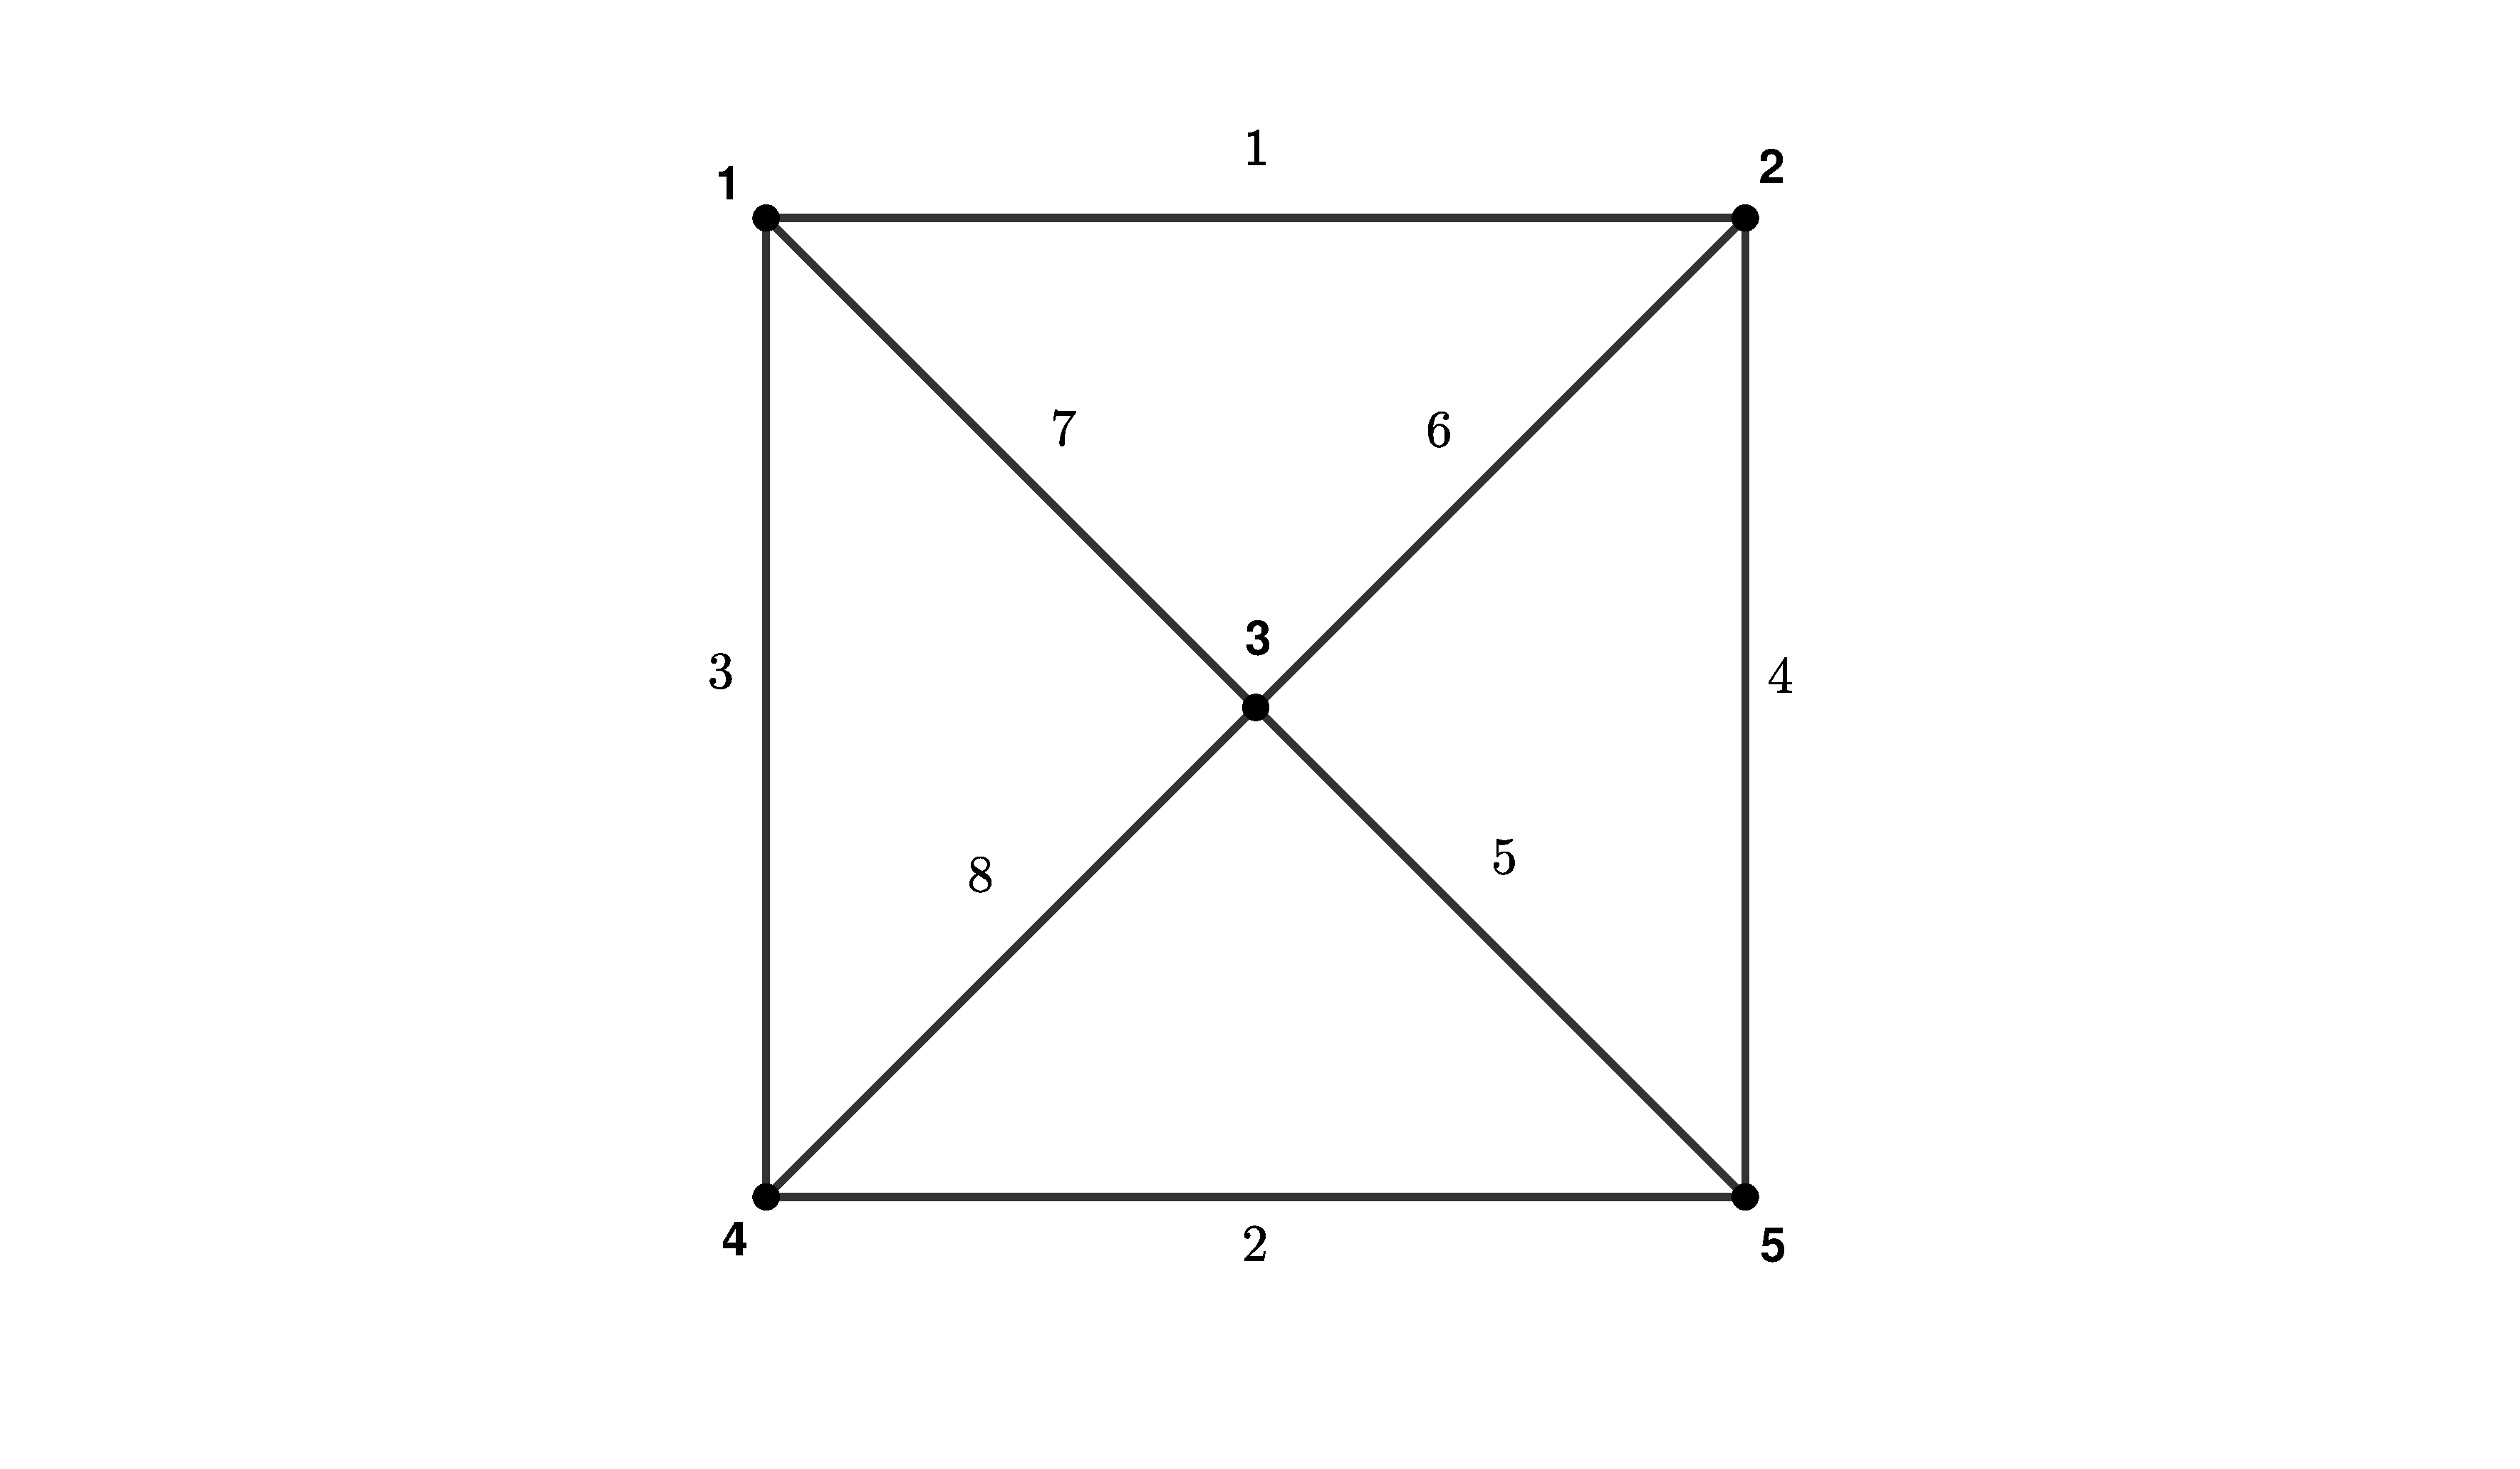
\includegraphics[scale = 0.15]{../图/12.1.1}
	\end{figure}
\end{example}

\begin{solution}
	边依权排列如下
	\begin{table}[H]
		\centering
		\begin{tabular}{c|cccccccc}
			\hline
			边 & $e_{12}$ & $e_{45}$ & $e_{14}$ & $e_{25}$ & $e_{35}$ & $e_{23}$ & $e_{13}$ & $e_{34}$ \\
			\hline
			权 & $1$ & $2$ & $3$ & $4$ & $5$ & $6$ & $7$ & $8$ \\ \hline
		\end{tabular}
	\end{table}
	在不产生圈的前提下依次加边,直至得到最小树。
	
	选取$e_{12}$,构成如下图
	\begin{figure}[H]
		\centering
		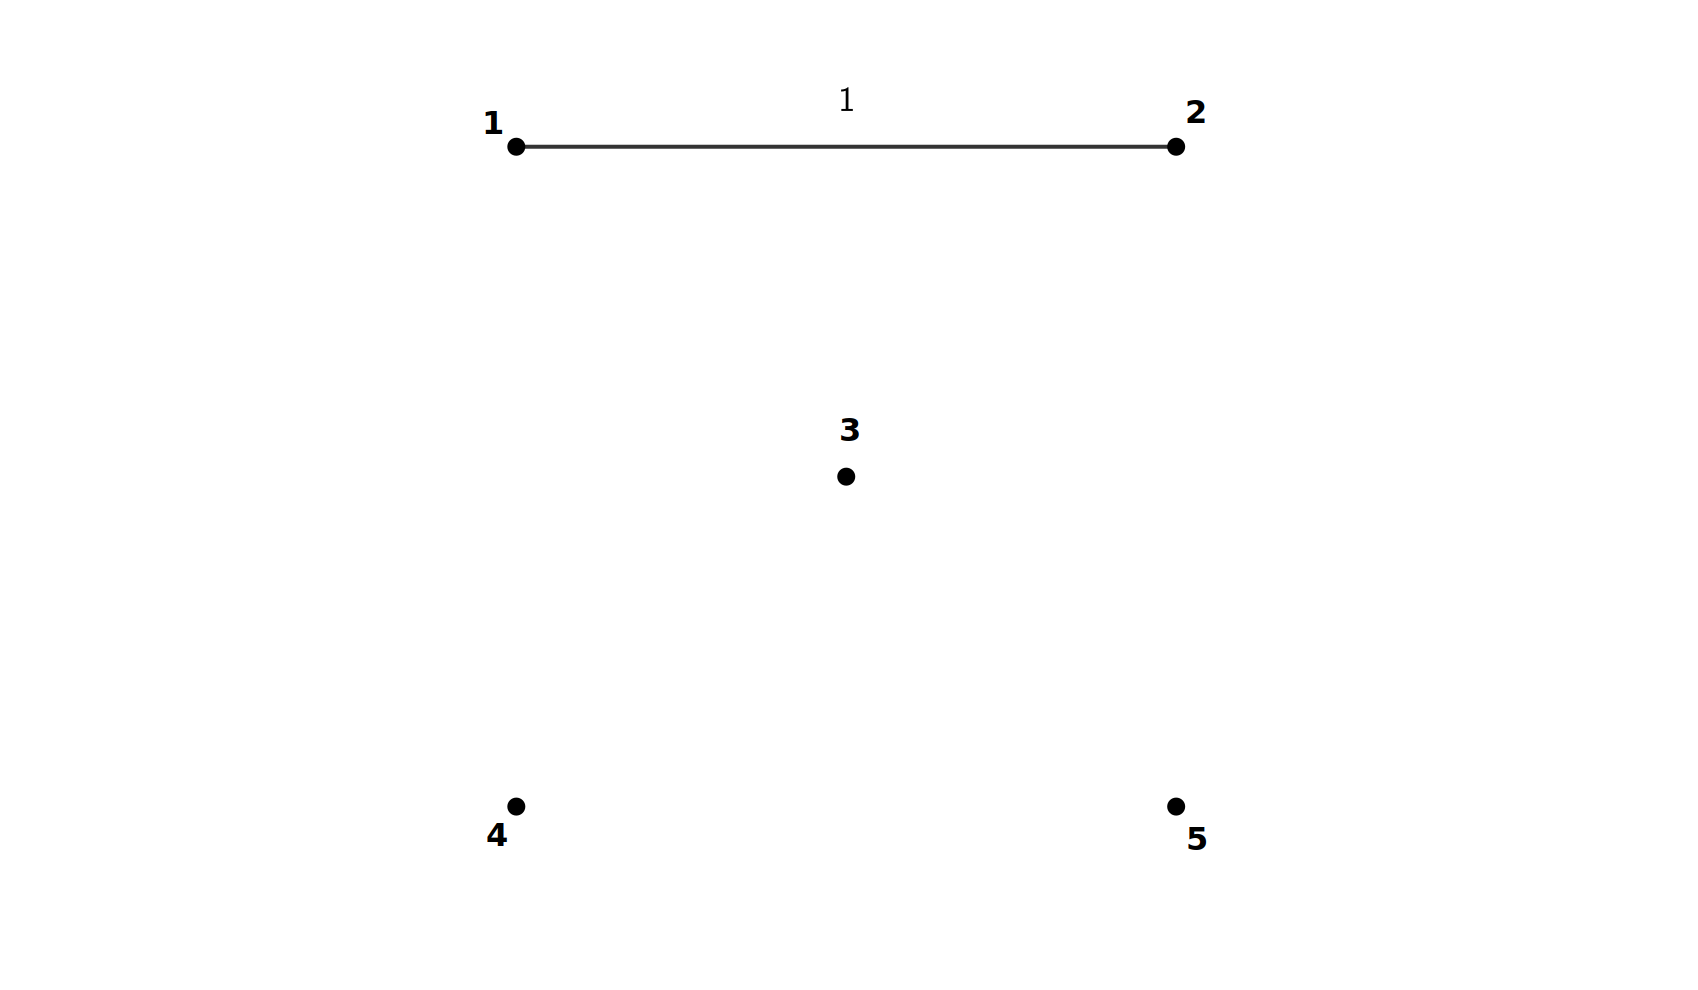
\includegraphics[scale = 0.15]{../图/12.1.2}
	\end{figure}
	
	选取$e_{45}$,构成如下图
	\begin{figure}[H]
		\centering
		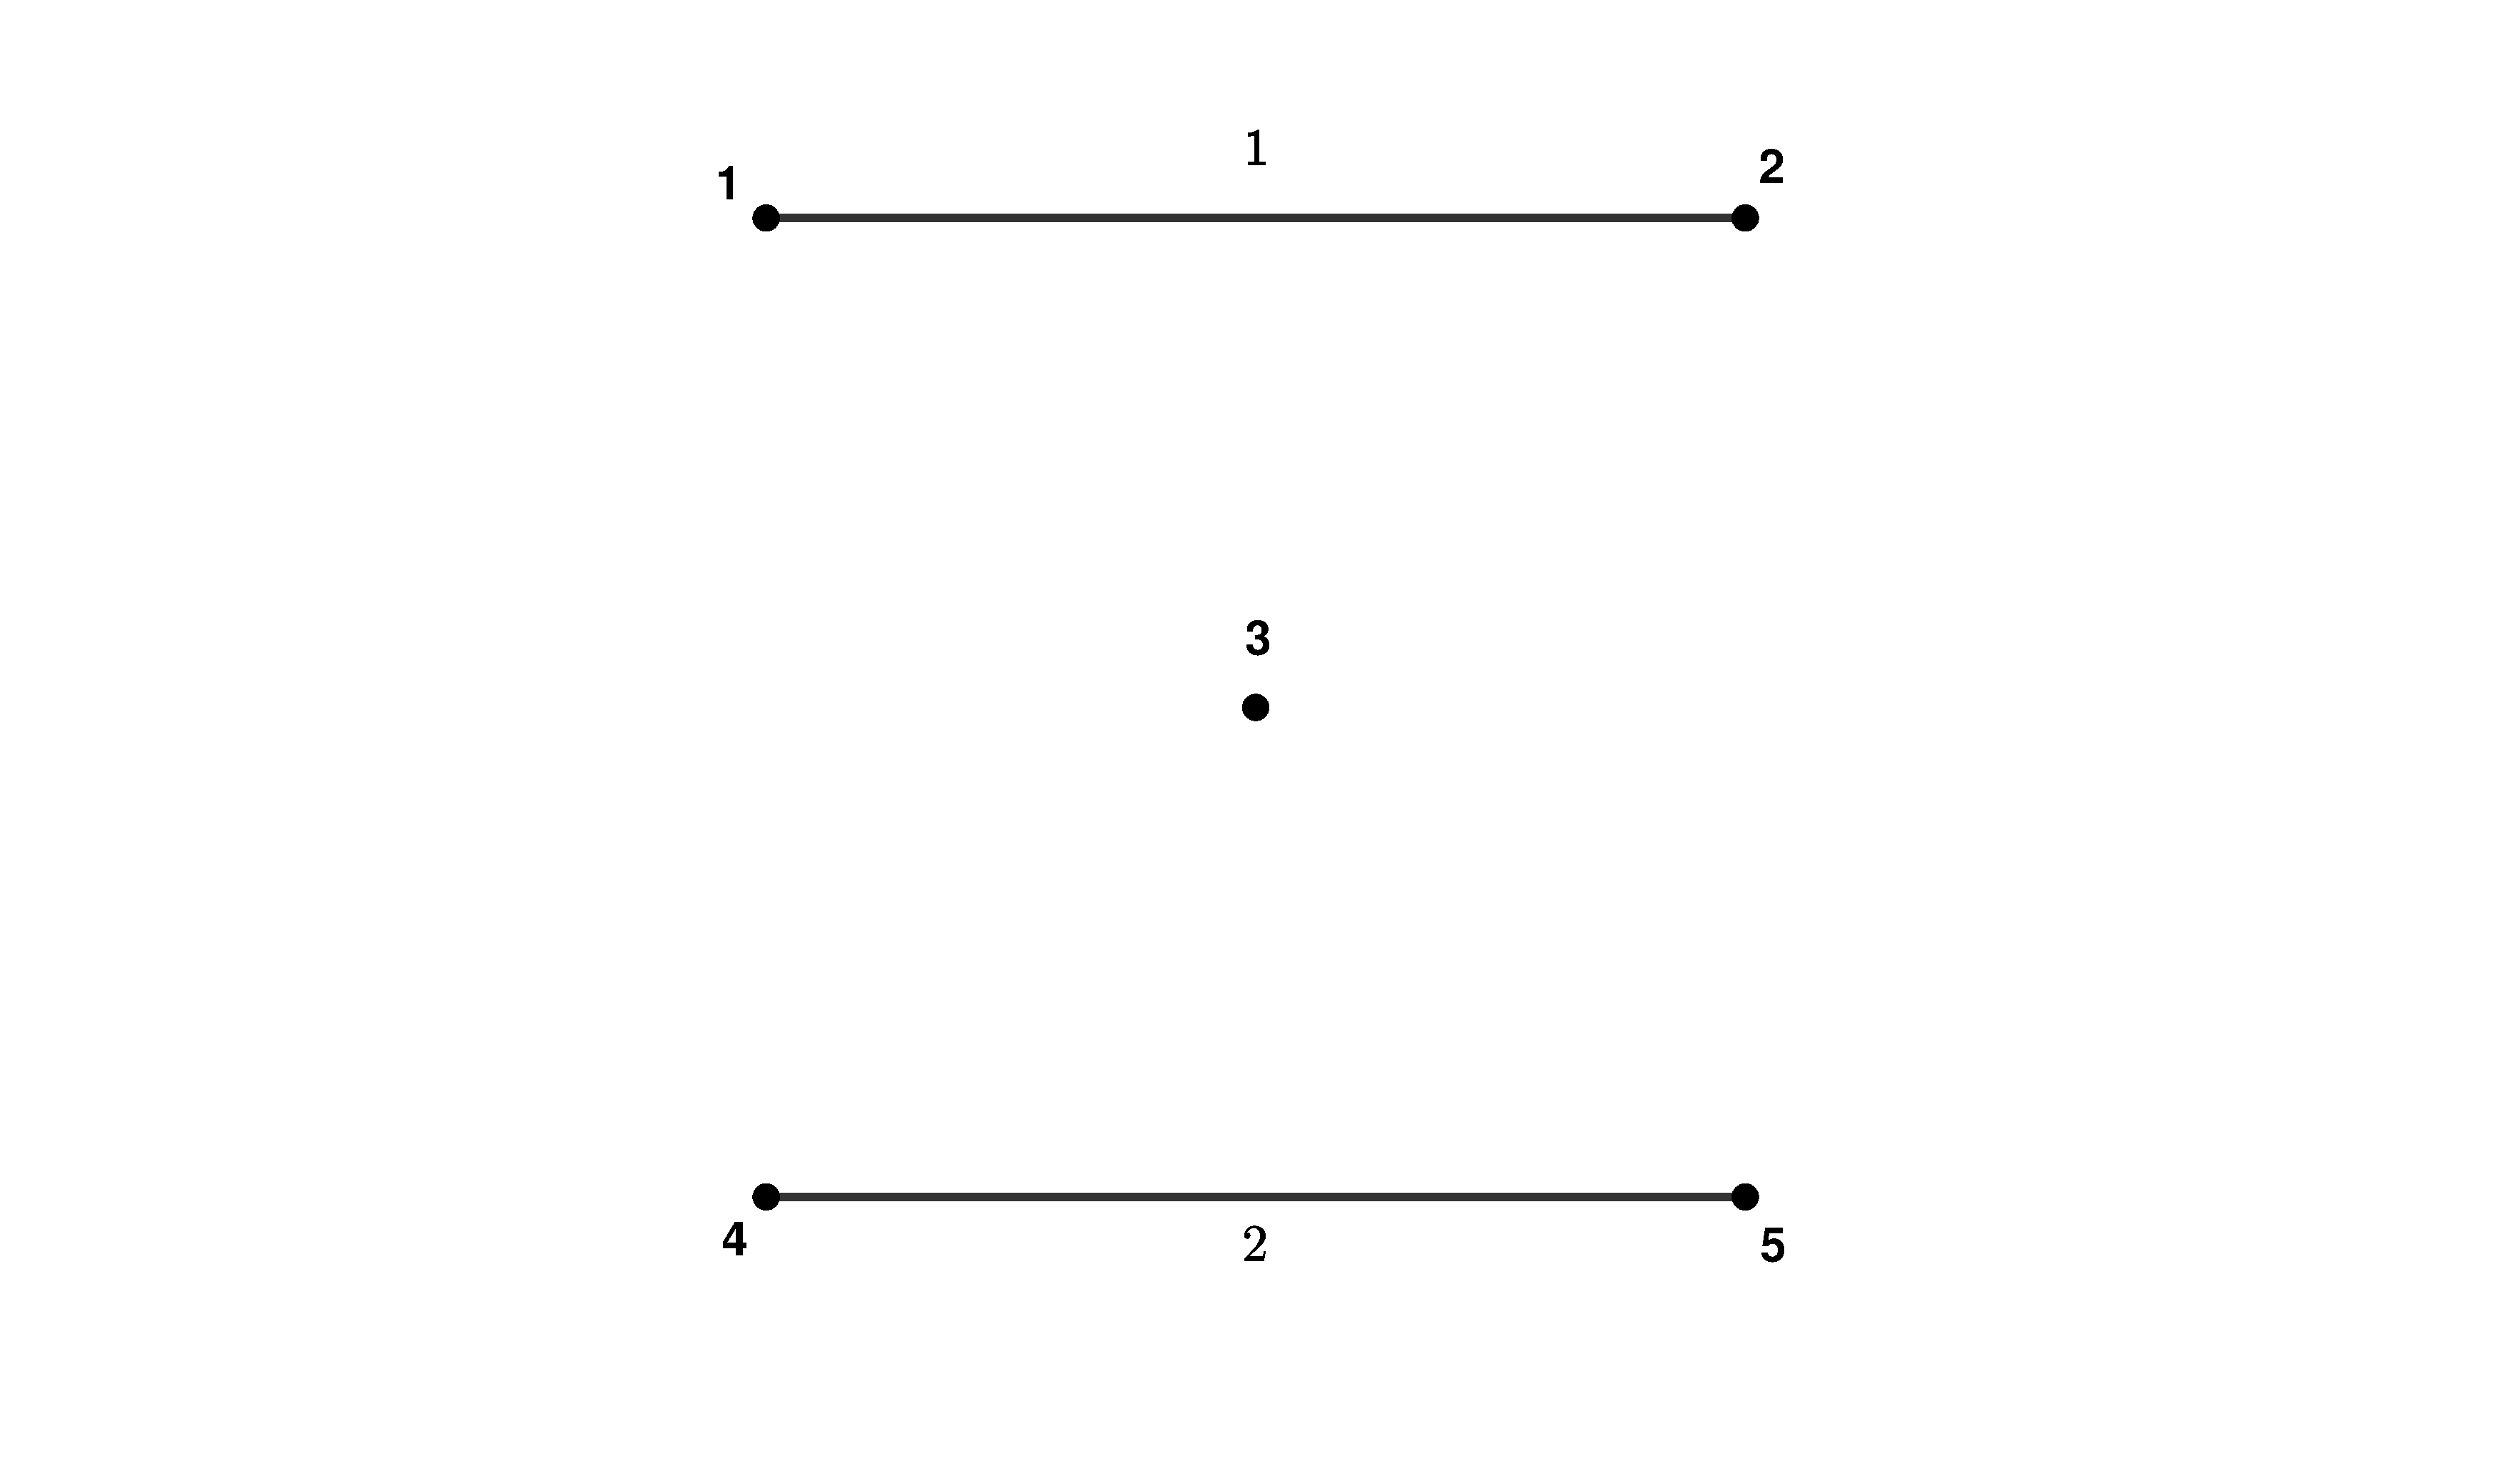
\includegraphics[scale = 0.15]{../图/12.1.3}
	\end{figure}
	
	选取$e_{14}$,构成如下图
	\begin{figure}[H]
		\centering
		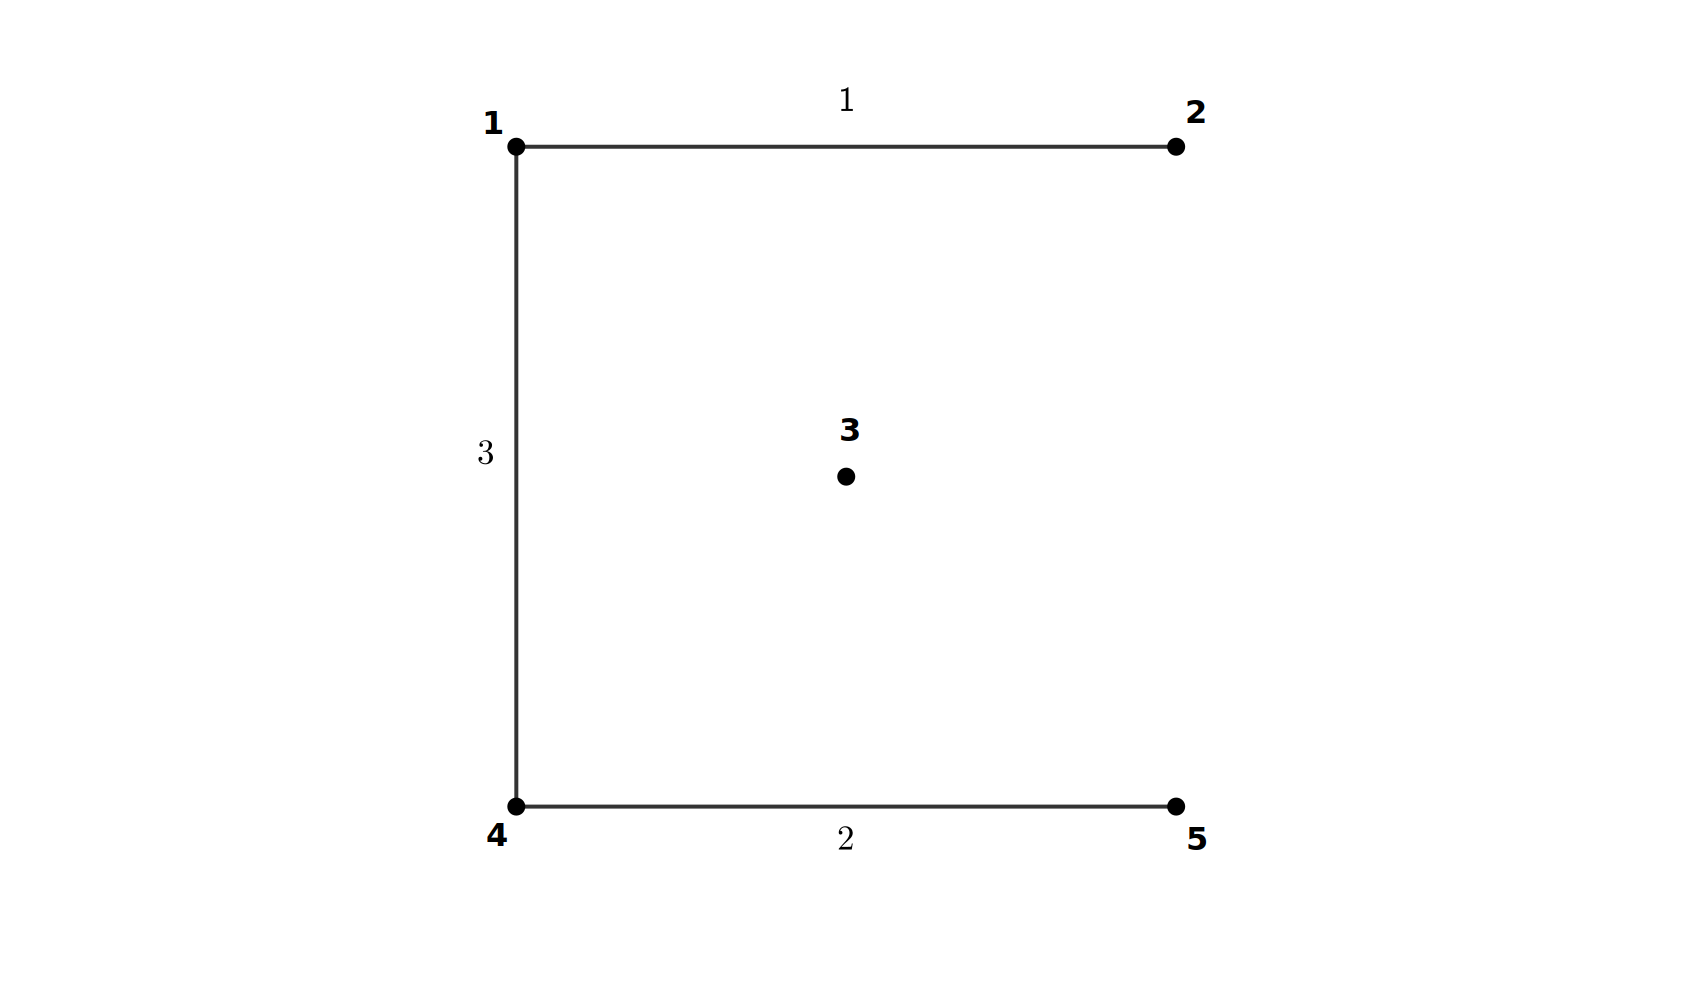
\includegraphics[scale = 0.15]{../图/12.1.4}
	\end{figure}
	
	若选取$e_{25}$,则构成回路$1\to 2\to 5\to 4\to 1$。选取$e_{35}$,构成如下图
	\begin{figure}[H]
		\centering
		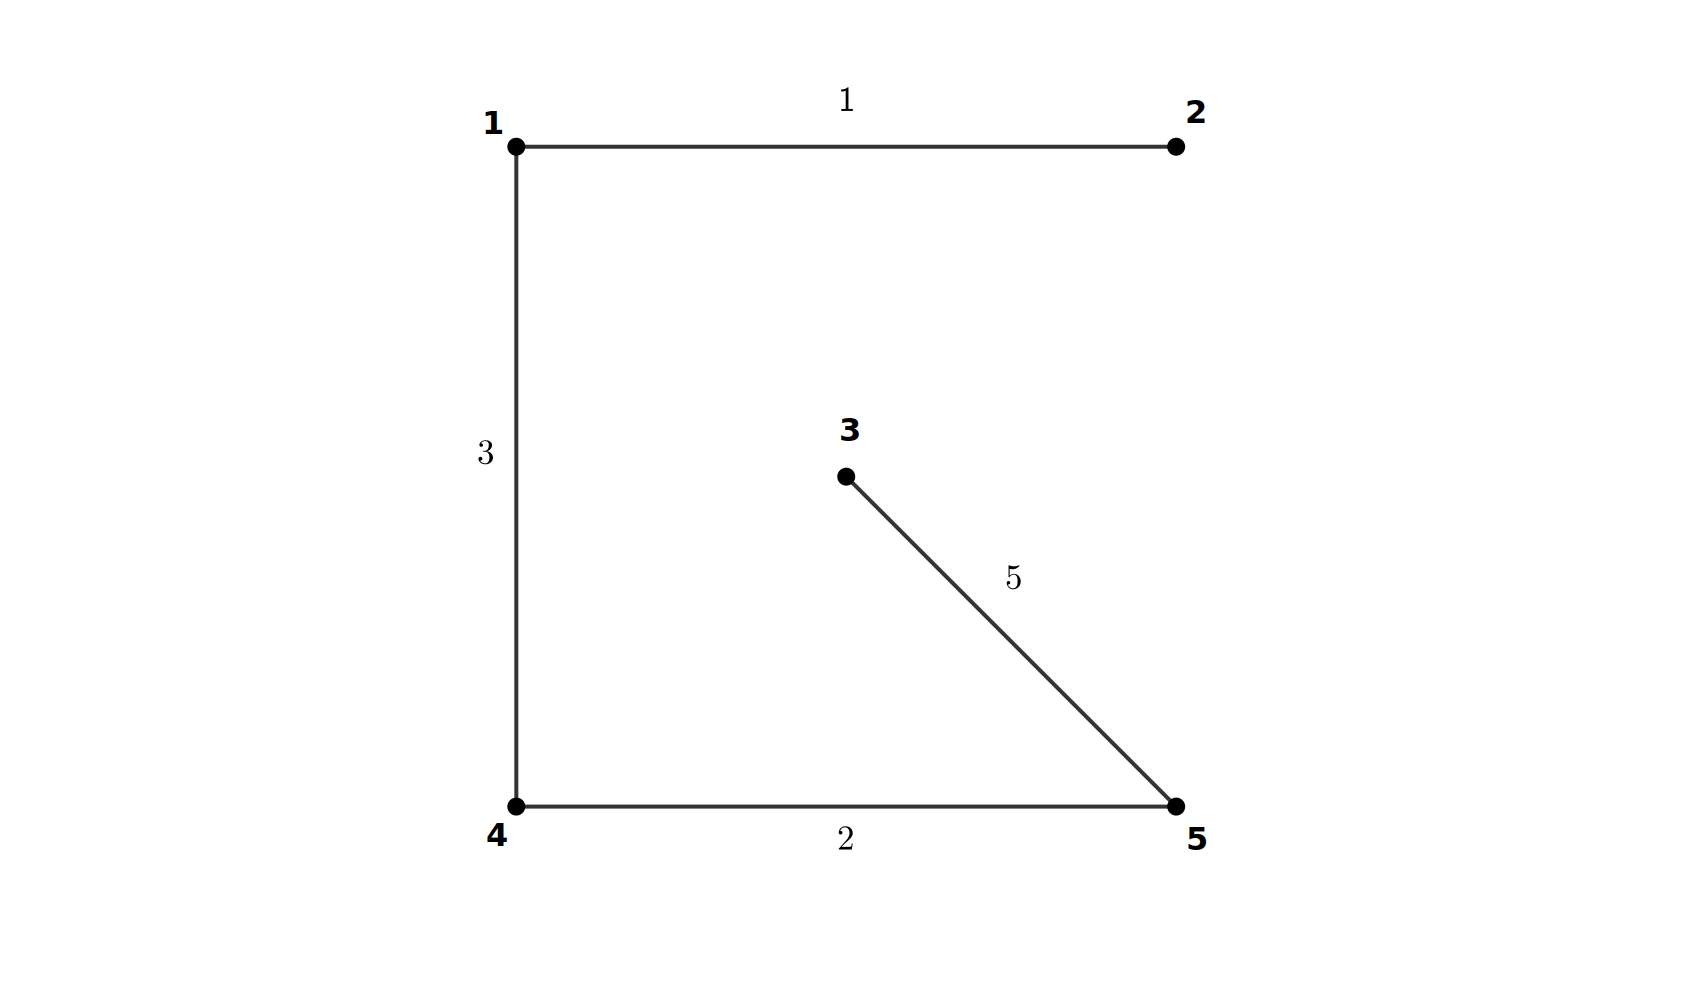
\includegraphics[scale = 0.15]{../图/12.1.5}
	\end{figure}
	此时已构成树,因此为最小树。
\end{solution}

\subsection{Dijkstra算法}

\begin{theorem}{Dijkstra算法}
	求网络$G(V,E,W)$的最小树,其中%
	$$
	V=\{ v_1,\cdots,v_n \},\qquad 
	\langle v_i,v_j \rangle = e_{ij},\qquad 
	W(e_{ij})=w_{ij}
	$$
	\begin{enumerate}
		\item 令%
		$$
		u_j\coloneqq w_{1j},\qquad 
		T\coloneqq \varnothing,\qquad
		R\coloneqq \{ v_1 \},\qquad 
		S\coloneqq \{ v_2,\cdots,v_n \}
		$$
		\item 取%
		$$
		u_k\coloneqq \min_{j\in S}\{ u_j \}=w_{ik}
		$$
		令%
		$$
		T\coloneqq T\cup\{ e_{ik} \},\qquad 
		R\coloneqq R\cup\{ v_k \},\qquad 
		S\coloneqq S\setminus\{ v_k \}
		$$
		\item 若$S=\varnothing$,停止;否则,令%
		$$
		u_j\coloneqq \min\{ u_j,w_{kj} \},\qquad j\in S
		$$
		转至第2步。
	\end{enumerate}
\end{theorem}

\begin{example}
	用Dijkstra算法求解下图所示网络的最小树。
	\begin{figure}[H]
		\centering
		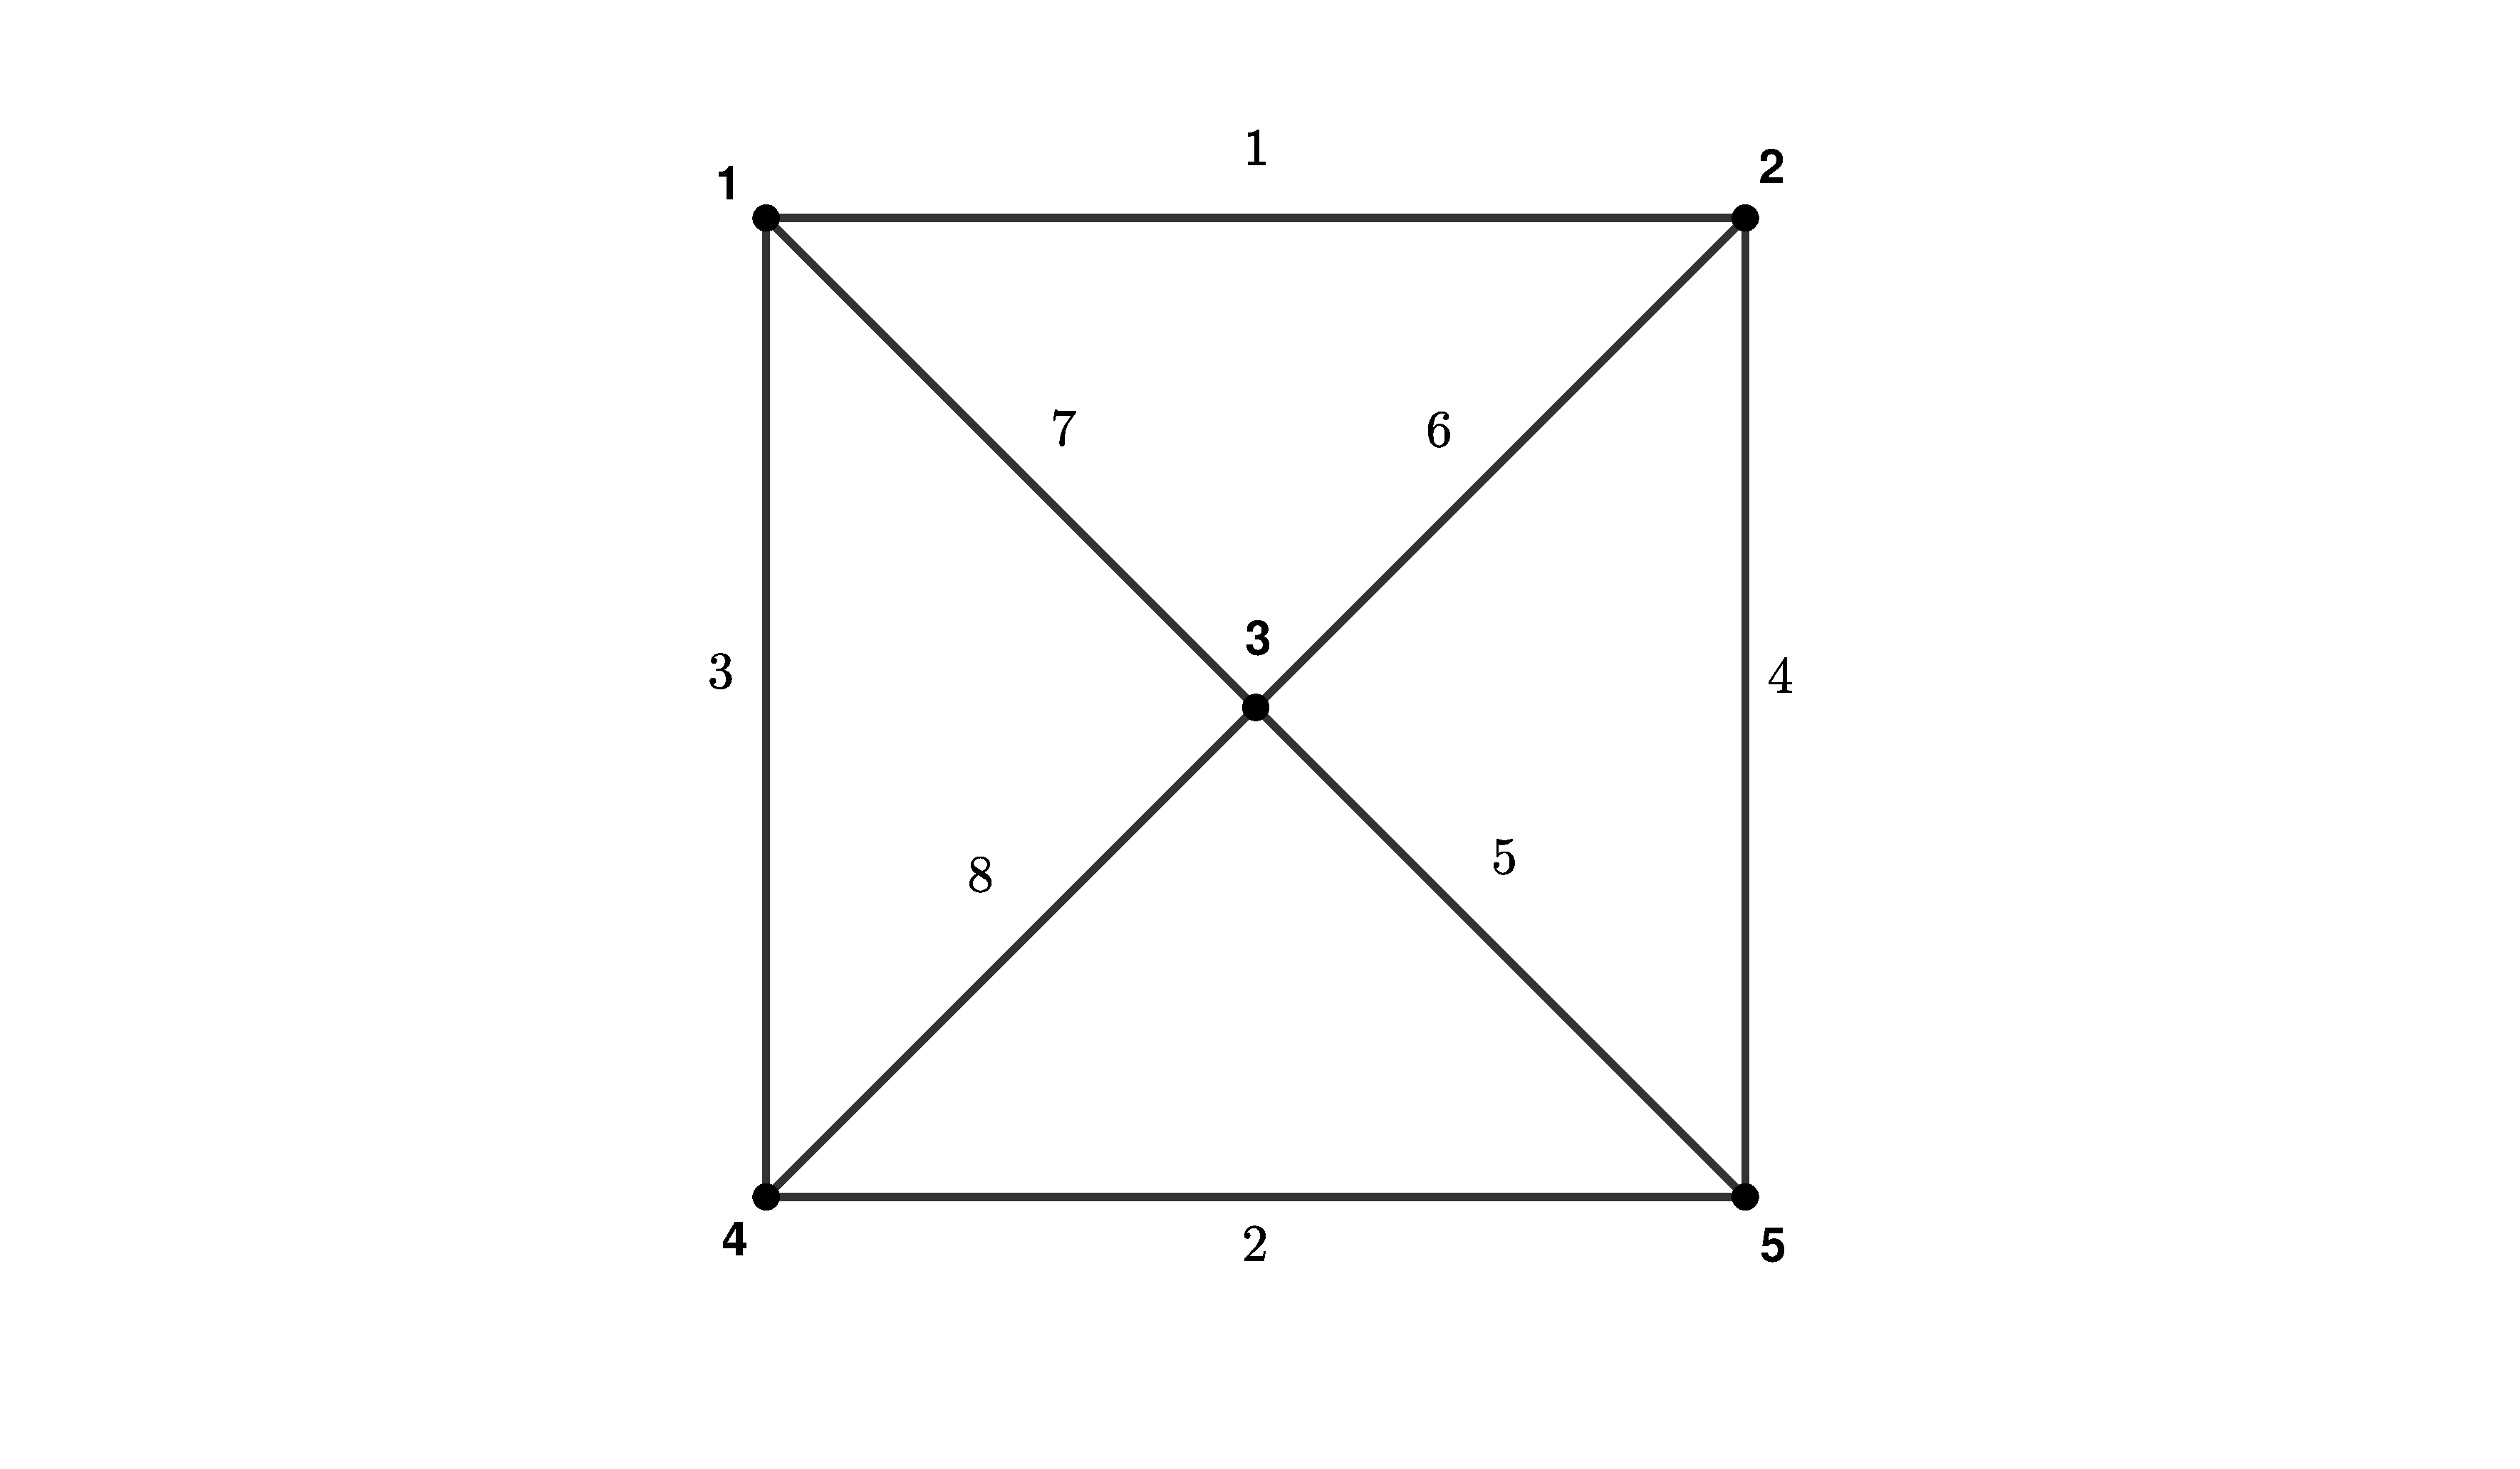
\includegraphics[scale = 0.15]{../图/12.1.1}
	\end{figure}
\end{example}

\begin{solution}
	选取点$1$为起始点,作割集
	\begin{figure}[H]
		\centering
		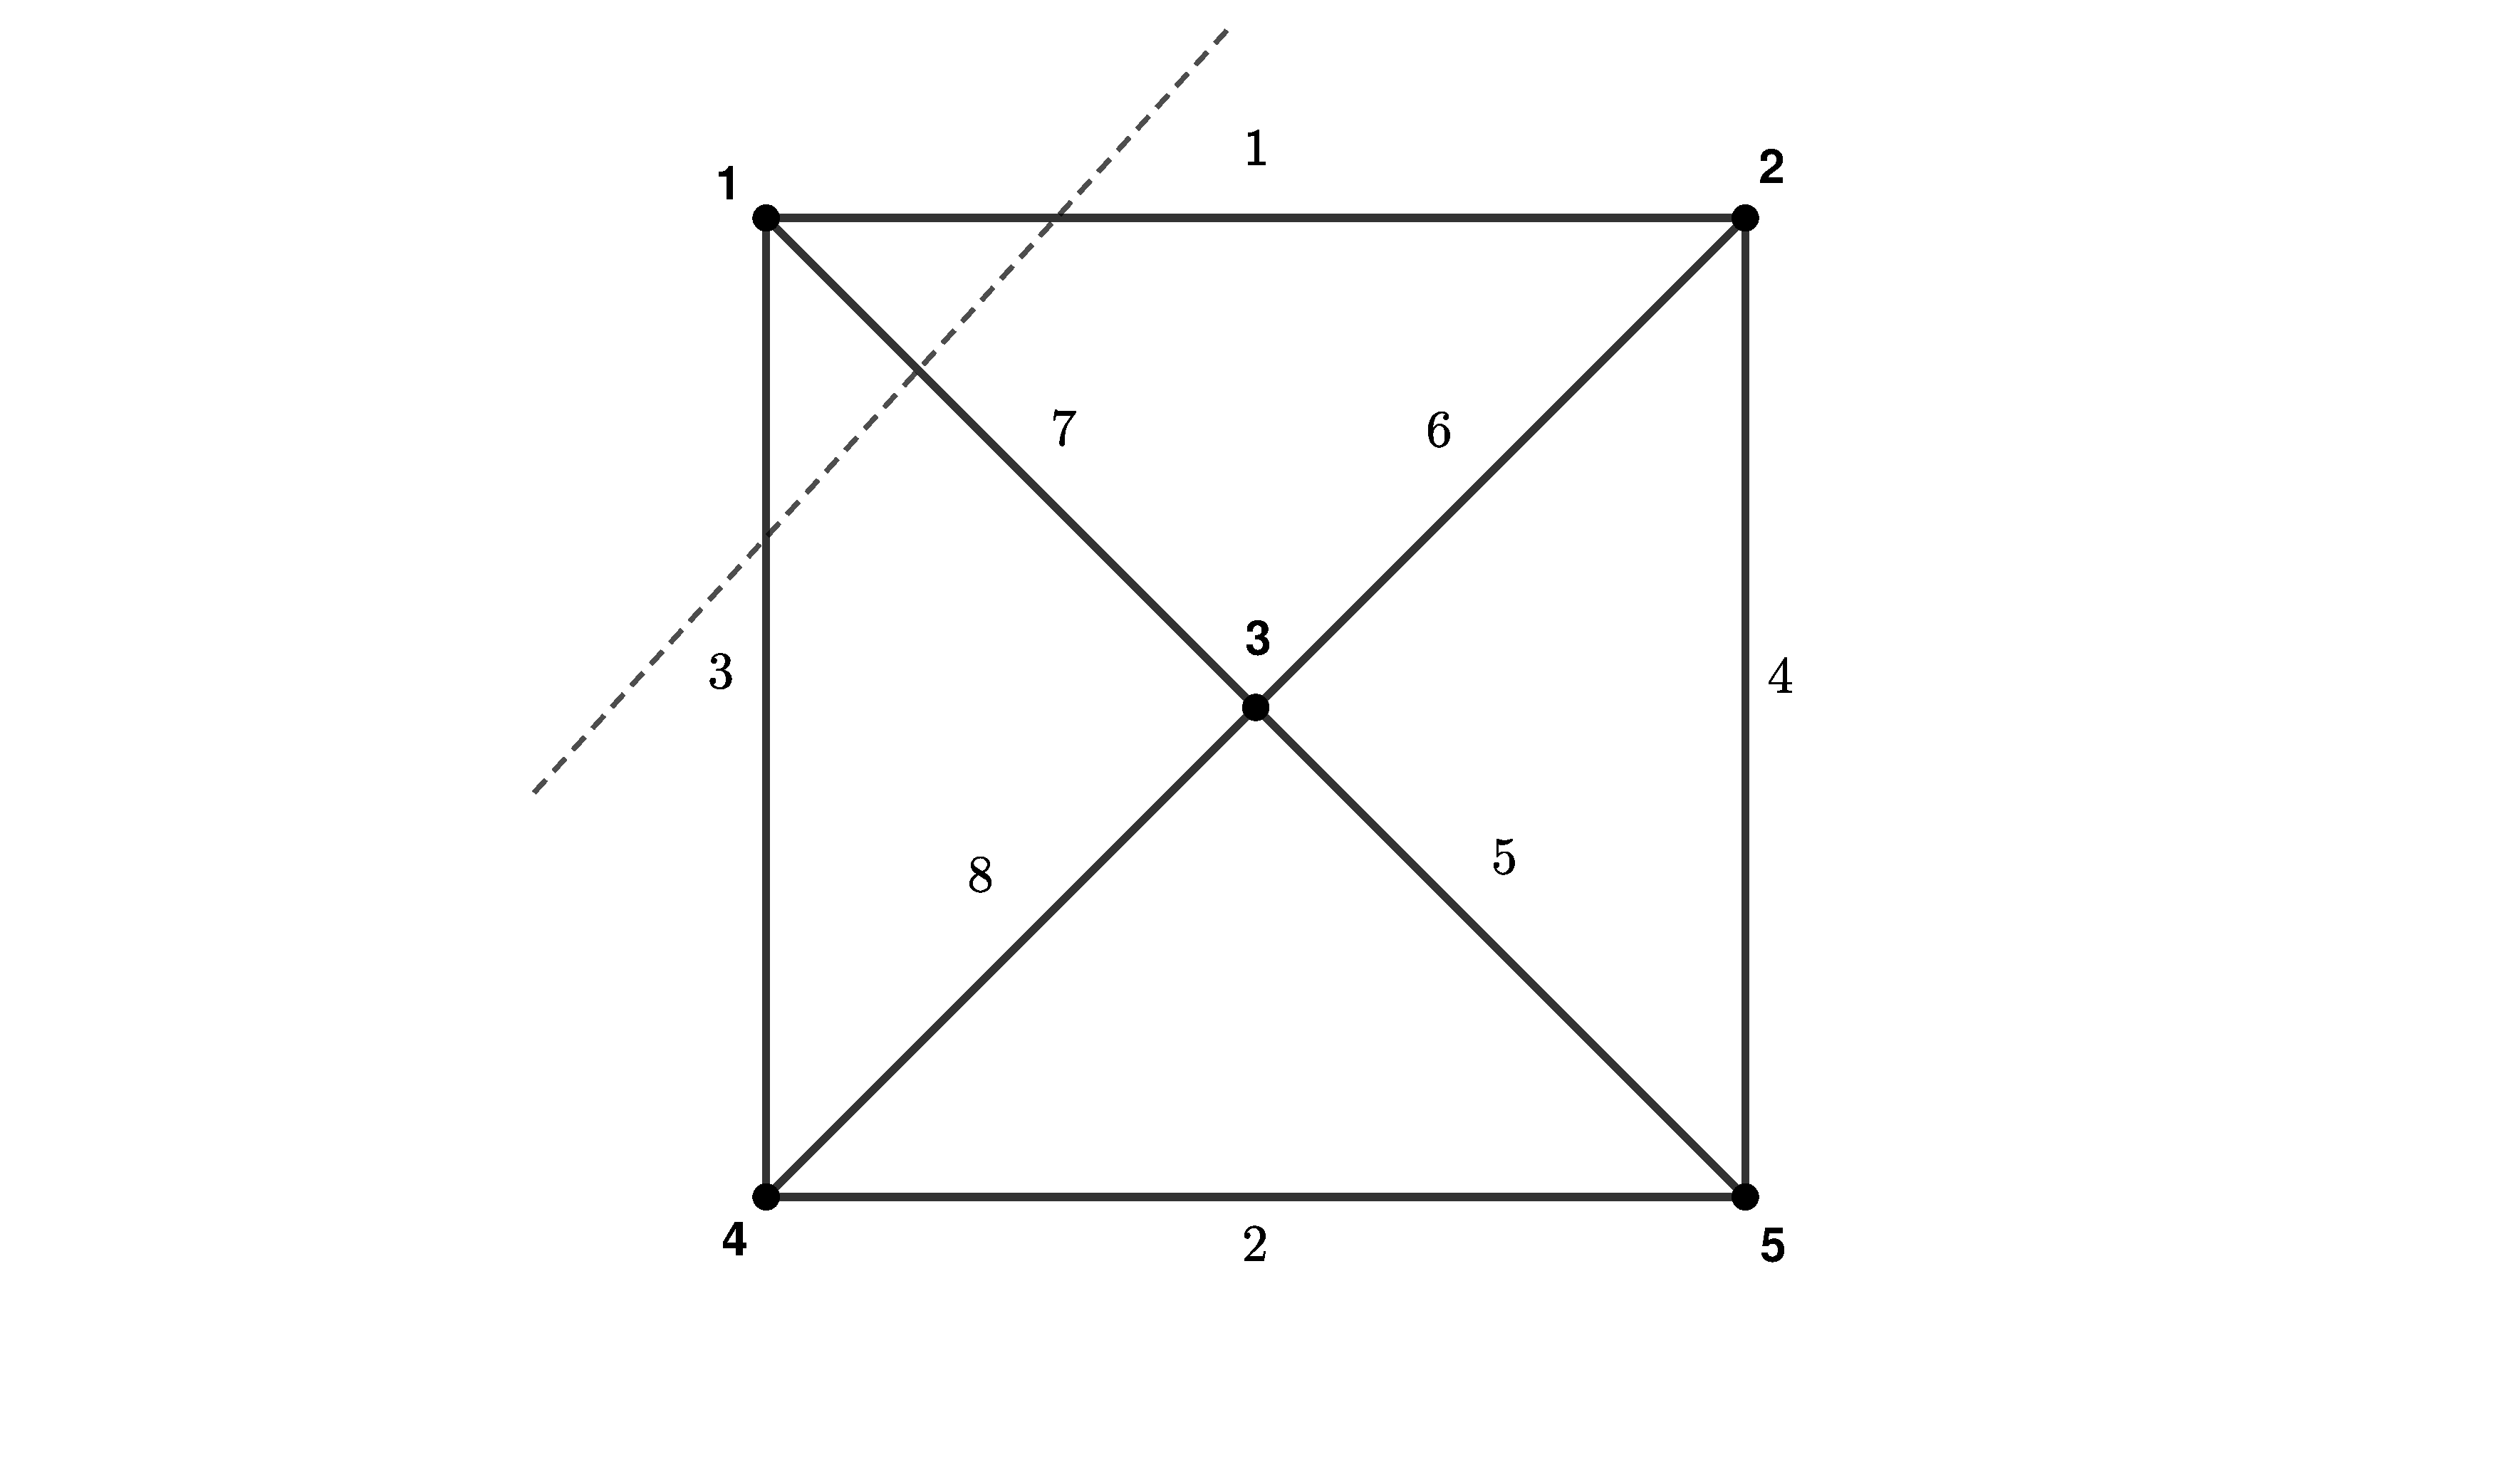
\includegraphics[scale = 0.15]{../图/12.2.1}
	\end{figure}
	
	选取边$e_{12}$,作割集
	\begin{figure}[H]
		\centering
		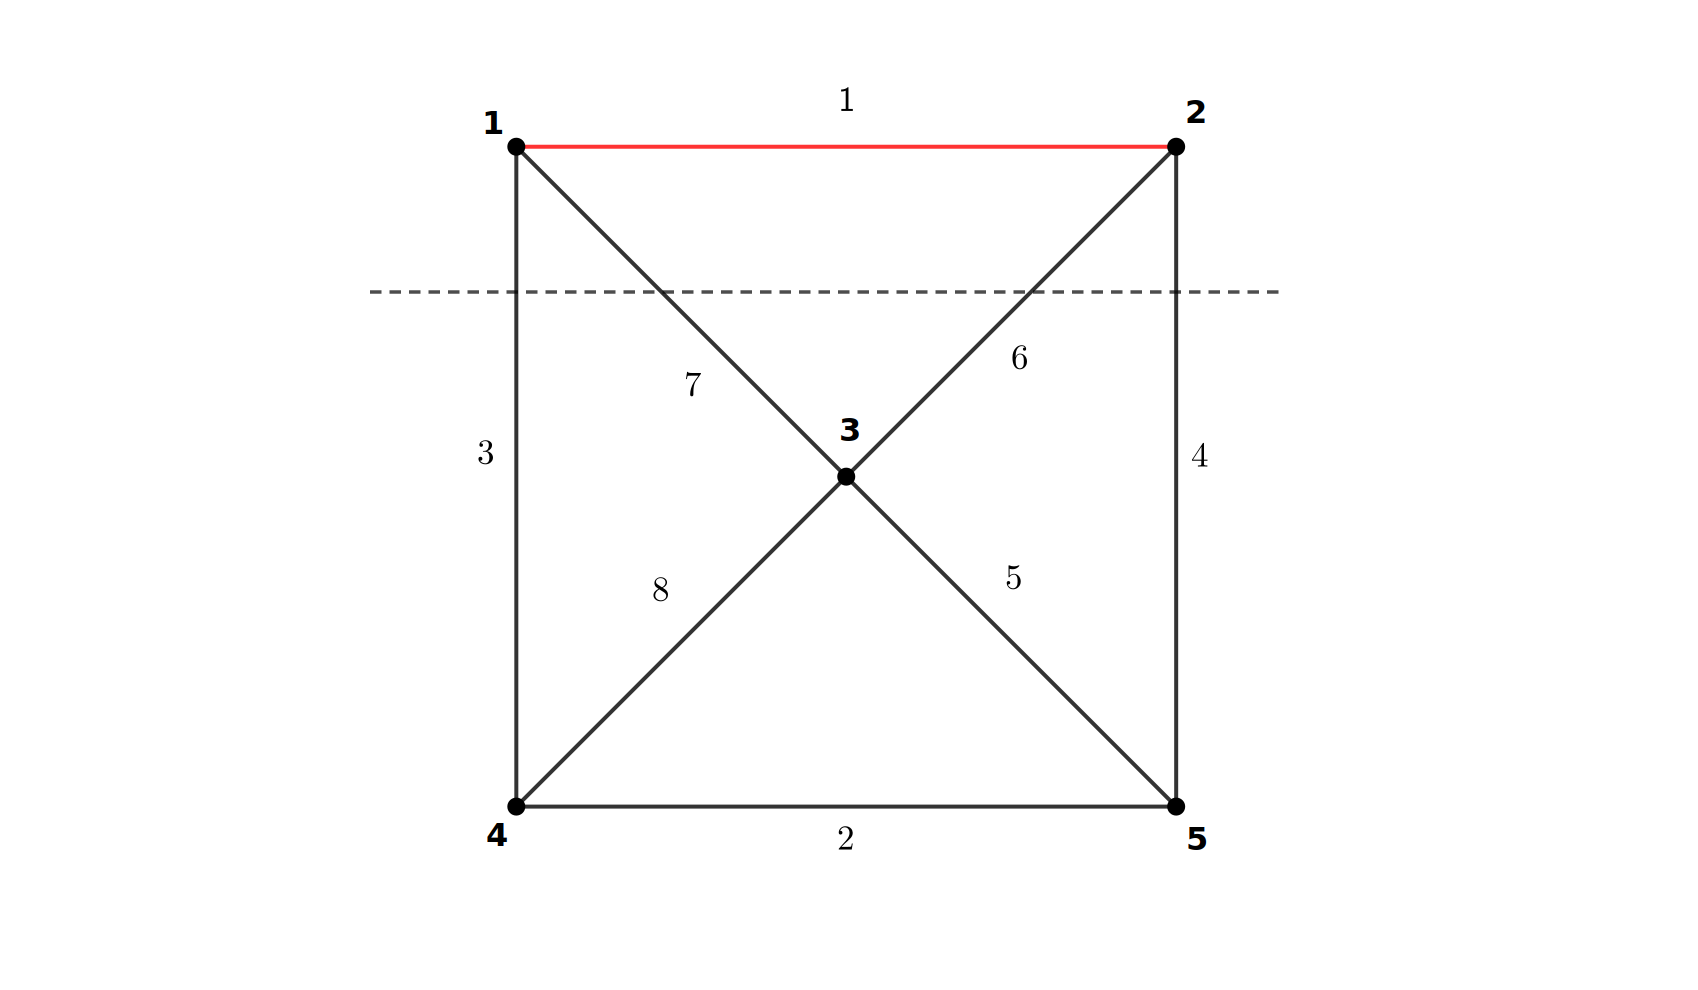
\includegraphics[scale = 0.15]{../图/12.2.2}
	\end{figure}
	
	选取边$e_{14}$,作割集
	\begin{figure}[H]
		\centering
		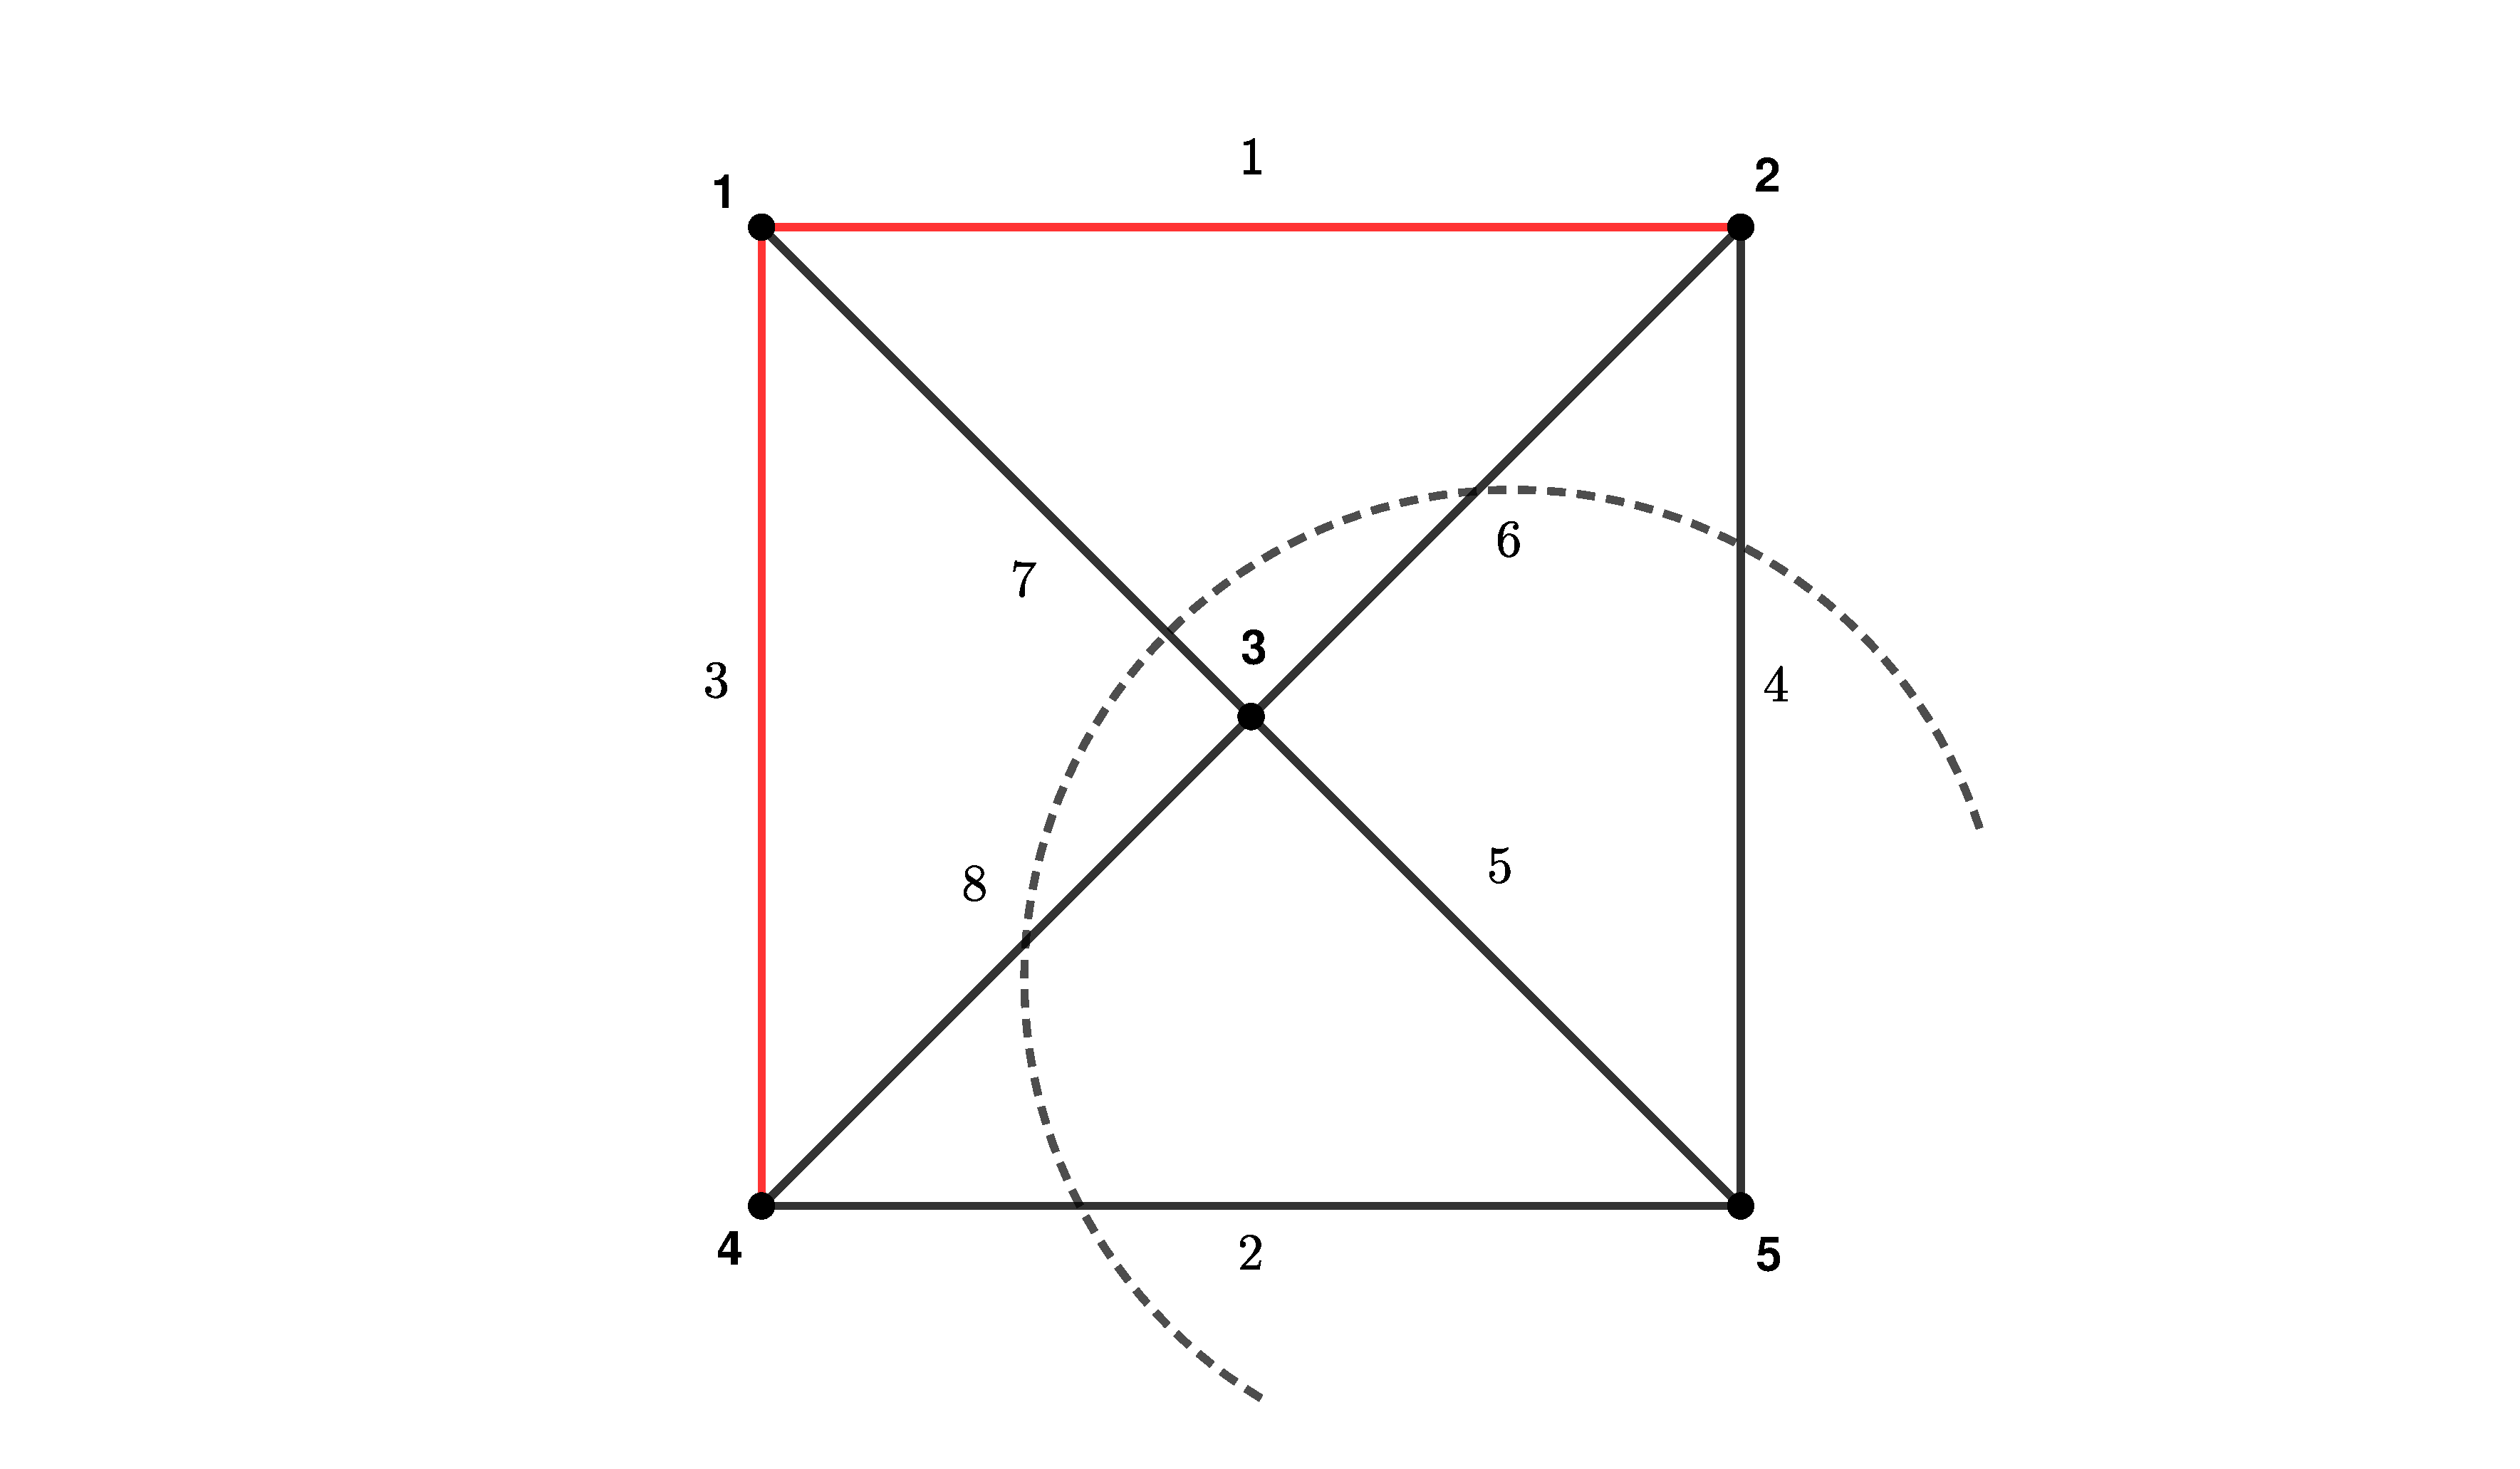
\includegraphics[scale = 0.15]{../图/12.2.3}
	\end{figure}
	
	选取边$e_{45}$,作割集
	\begin{figure}[H]
		\centering
		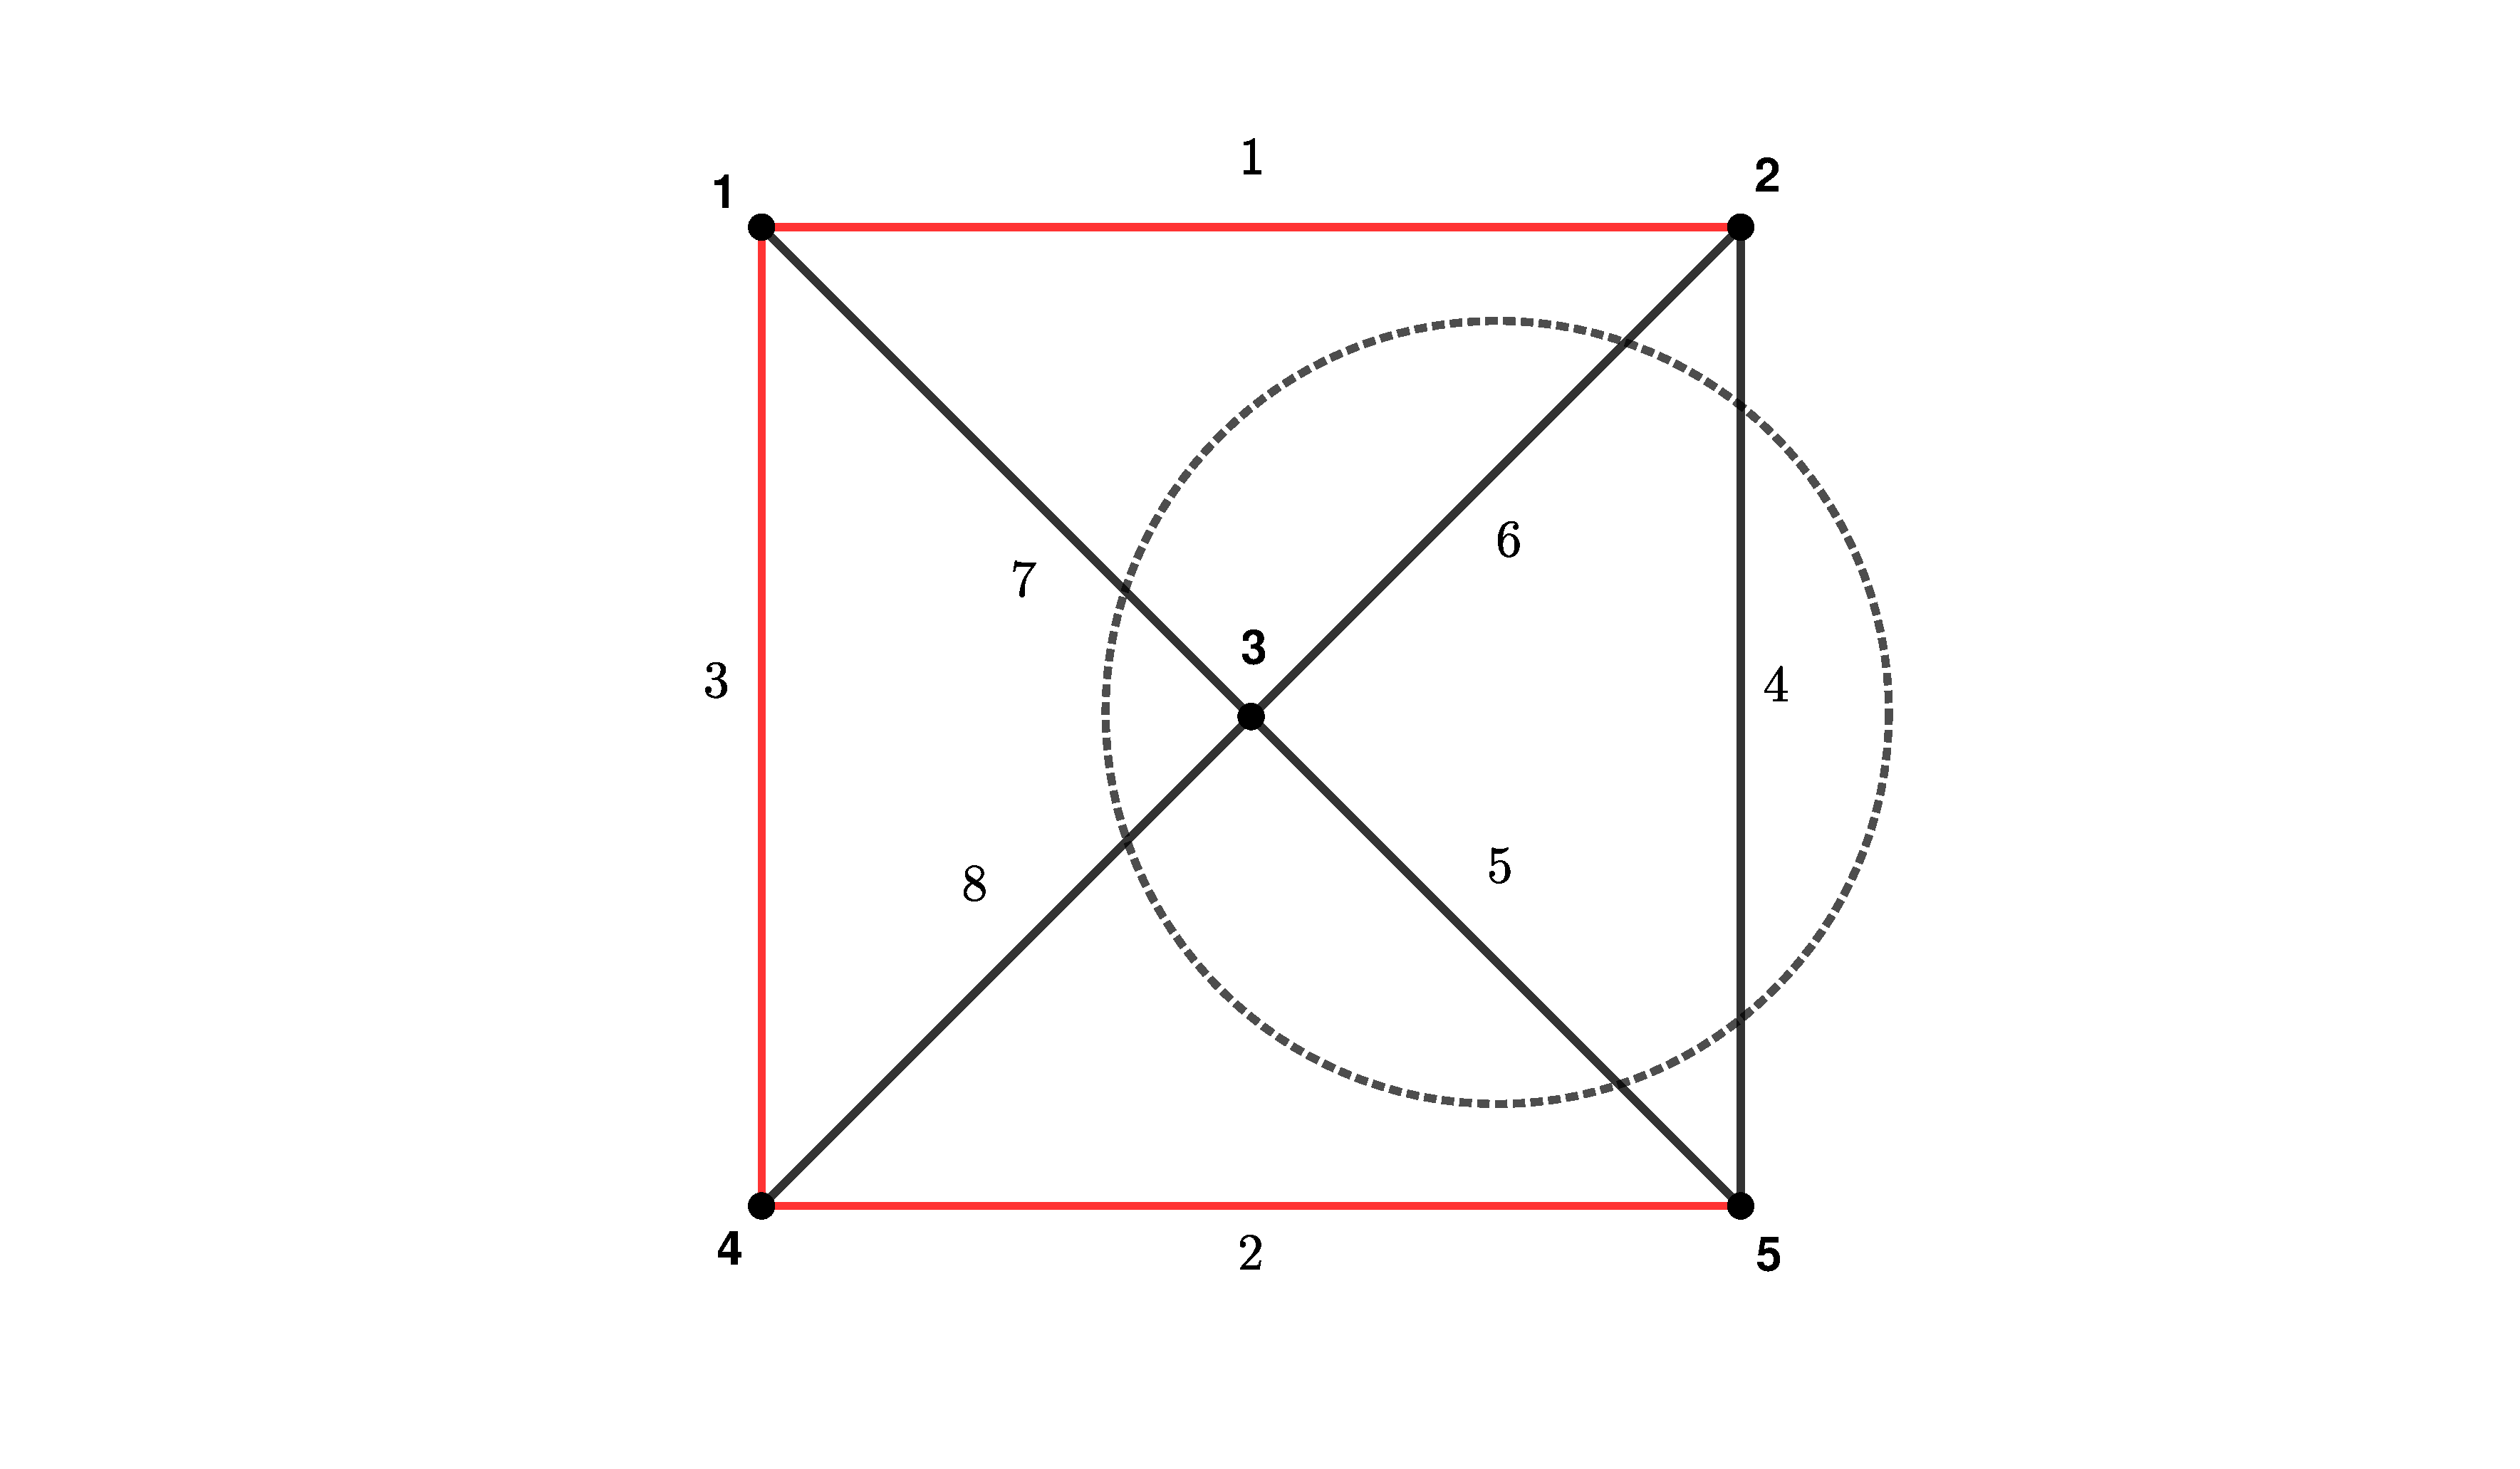
\includegraphics[scale = 0.15]{../图/12.2.4}
	\end{figure}
	
	选取边$e_{35}$,构成最小树
	\begin{figure}[H]
		\centering
		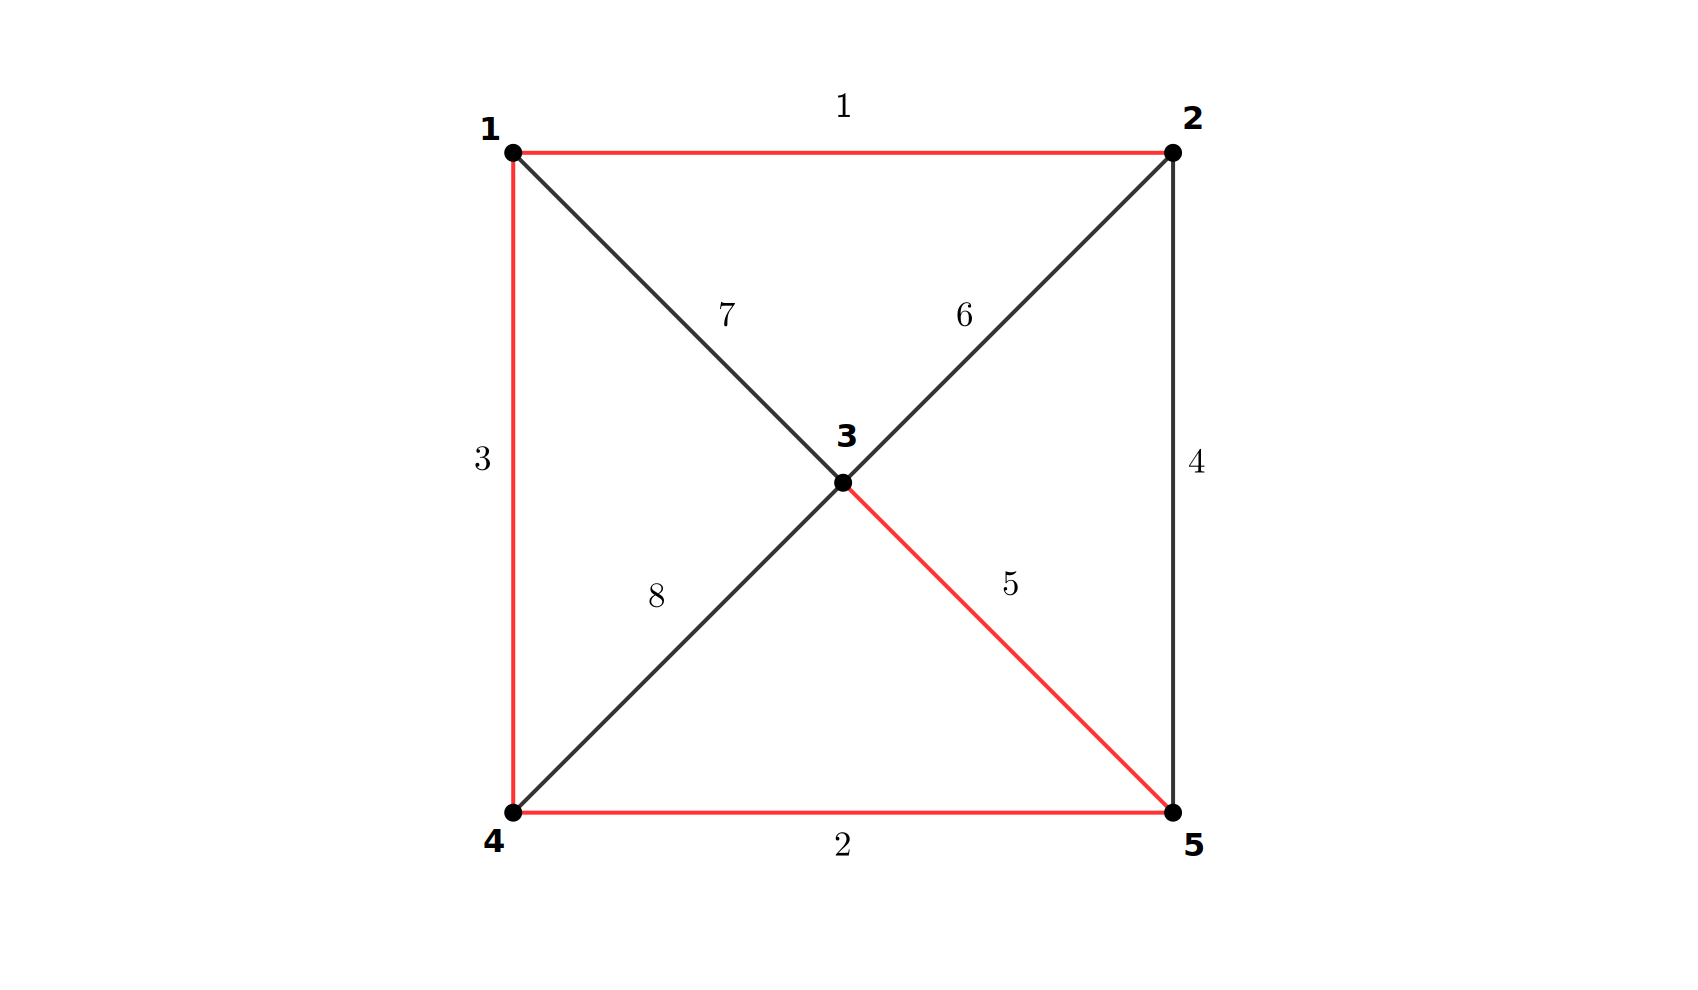
\includegraphics[scale = 0.15]{../图/12.2.5}
	\end{figure}
\end{solution}

\section{最短有向路问题}

\begin{theorem}{Dijkstra算法}
	对于正权有向网络$G=(V,E,W)$,求解点$1$到其他各点最短有向路径。
	\begin{enumerate}
		\item 令%
		$$
		u_1\col 0,\qquad 
		u_j\col w_{1j},\qquad 
		2\le j \le n,\qquad 
		P\col \{ 1 \},\qquad
		T\col \{ 2,\cdots,n \}
		$$
		\item 在$T$中寻找一点$k$,使得成立%
		$$
		u_k=\min_{j\in T}\{ u_j \}
		$$
		令%
		$$
		P\col P\cup\{ k \},\qquad 
		T\col T\setminus\{ k \}
		$$
		若$T=\varnothing$,终止;否则,转至第3步。
		\item 对于$T$中每一点$j$,令%
		$$
		u_j=\min\{ u_j,u_k+w_{kj} \}
		$$
		转至第2步。
	\end{enumerate}
\end{theorem}

\begin{example}
	用Dijkstra算法求解下图所示有向网络中自点$1$到其他各点的最短有向路。
	\begin{figure}[H]
		\centering
		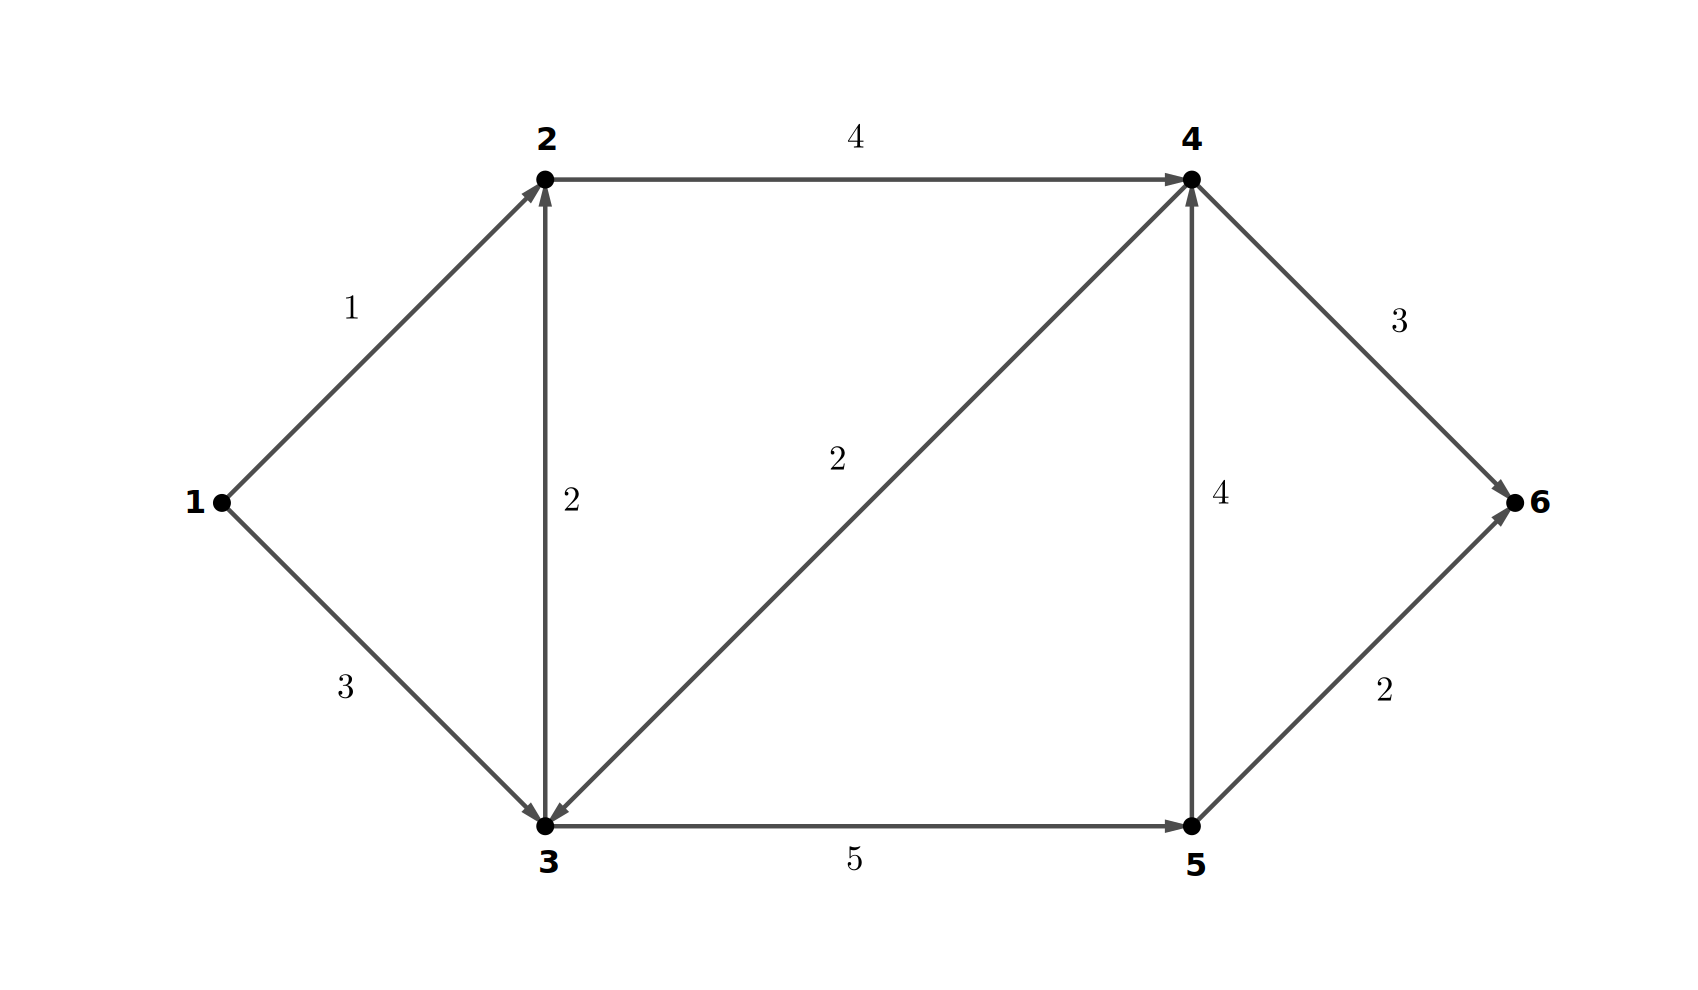
\includegraphics[scale = 0.15]{../图/13.1.1}
	\end{figure}
\end{example}

\begin{solution}
	作临时标号
	\begin{figure}[H]
		\centering
		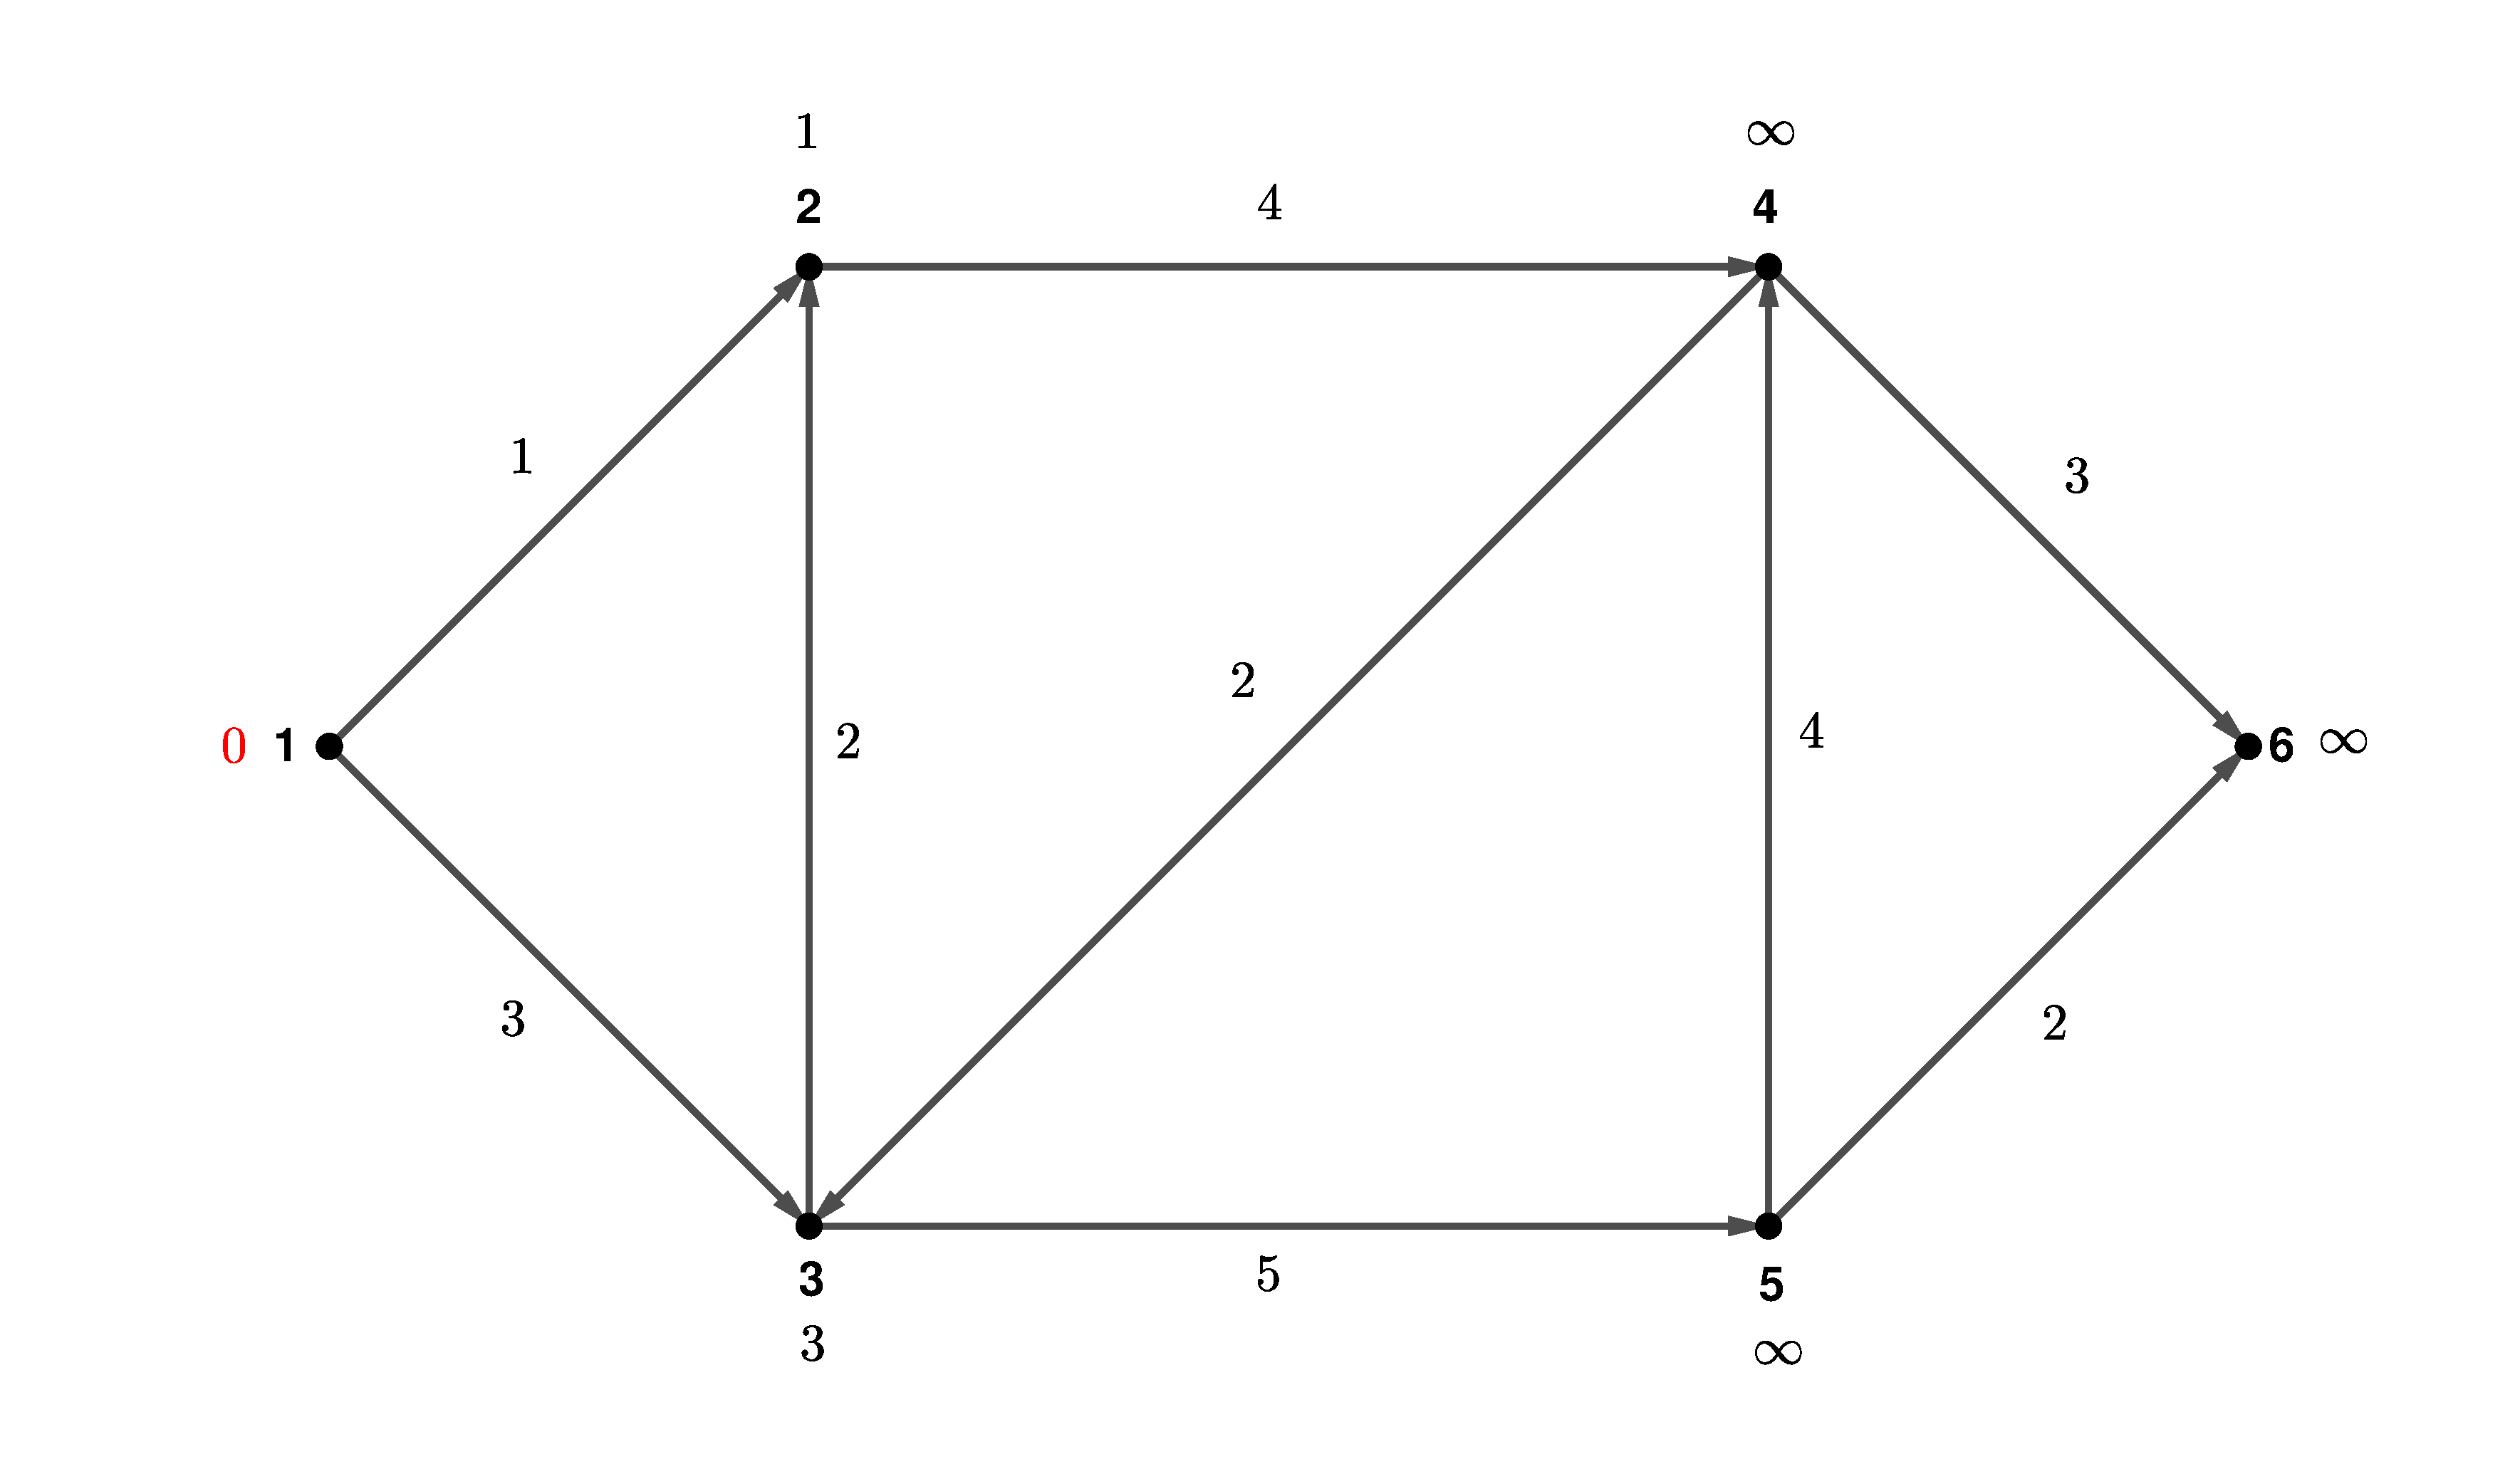
\includegraphics[scale = 0.15]{../图/13.1.2}
	\end{figure}
	
	选择点$2$的临时标号为永久标号,并更新其他点的临时标号。
	\begin{figure}[H]
		\centering
		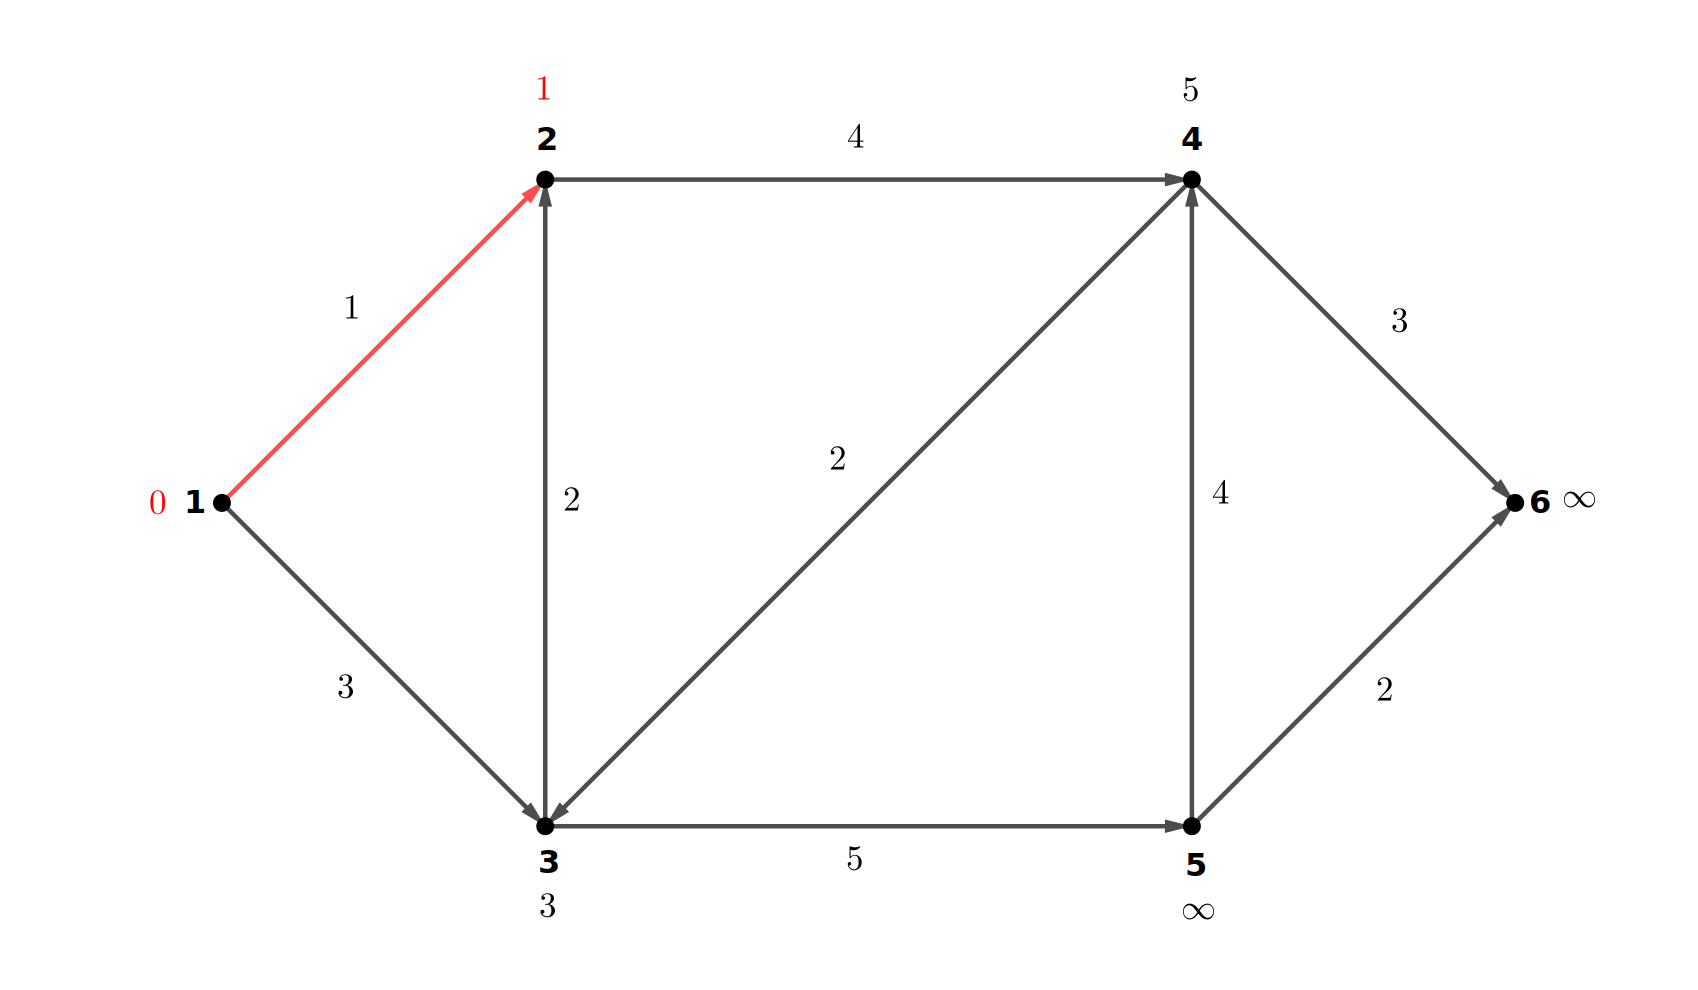
\includegraphics[scale = 0.15]{../图/13.1.3}
	\end{figure}
	
	选择点$3$​的临时标号为永久标号,并更新其他点的临时标号。
	\begin{figure}[H]
		\centering
		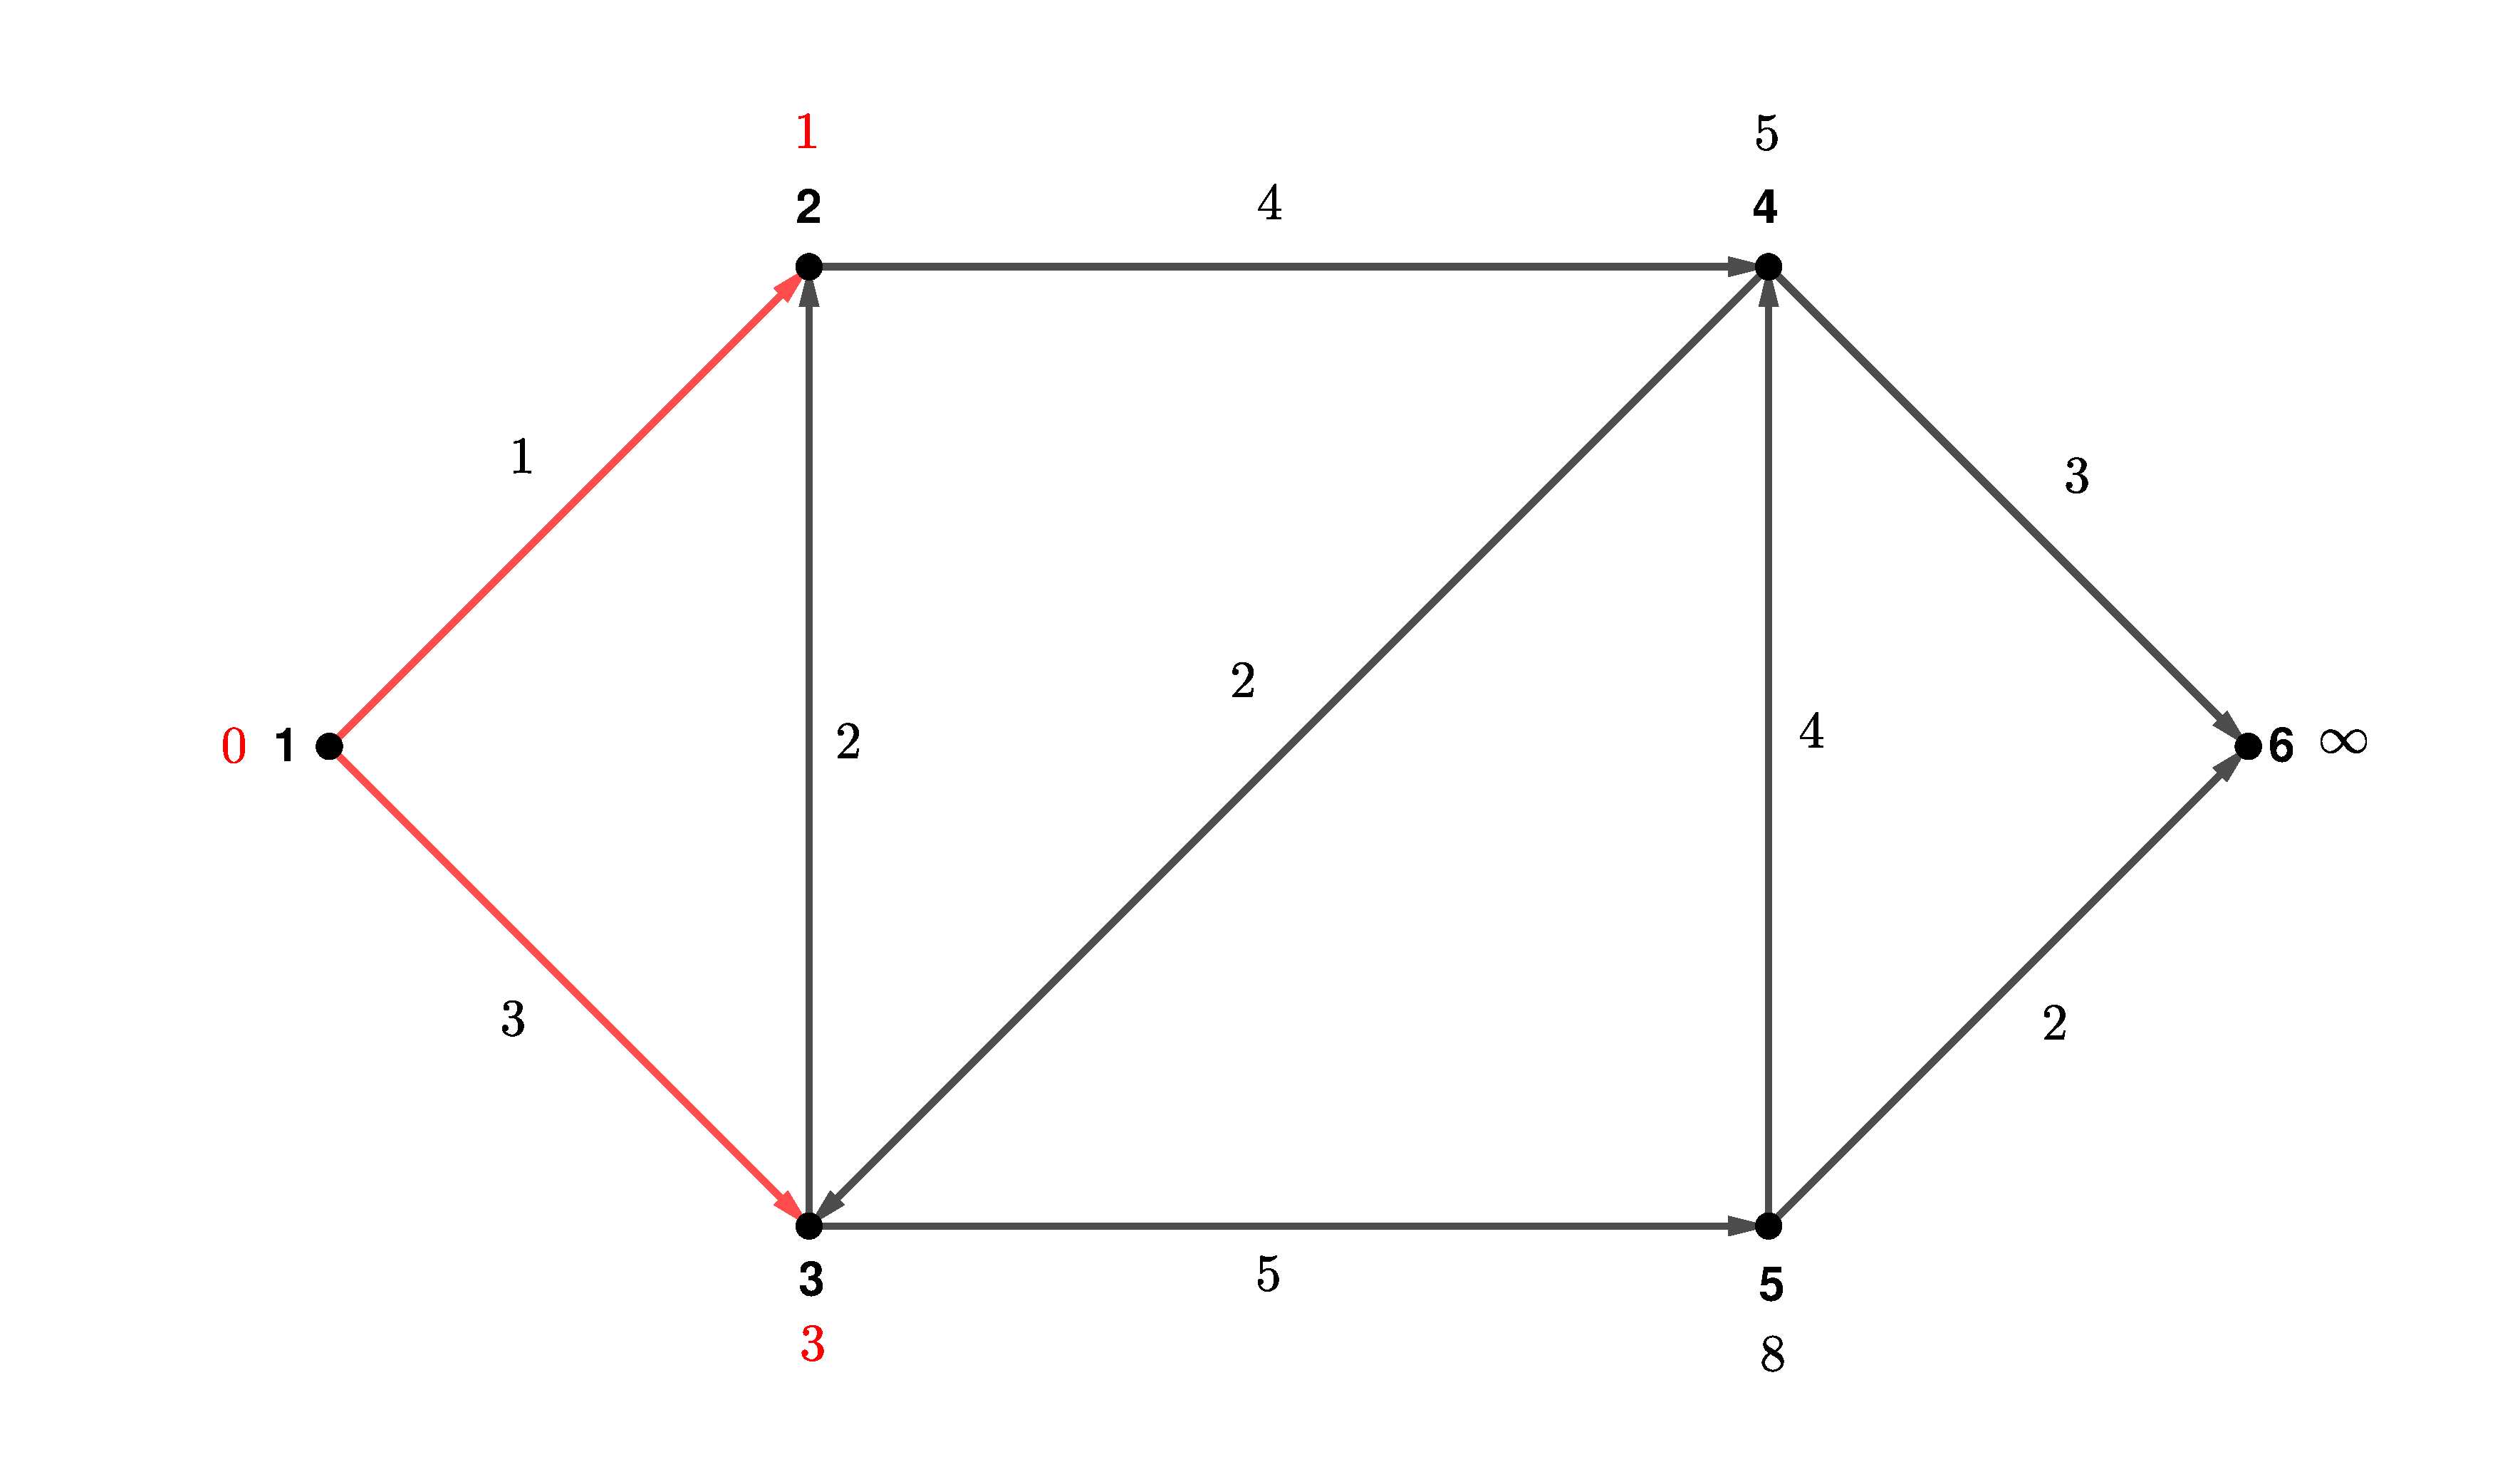
\includegraphics[scale = 0.15]{../图/13.1.4}
	\end{figure}
	
	选择点$4$​的临时标号为永久标号,并更新其他点的临时标号。
	\begin{figure}[H]
		\centering
		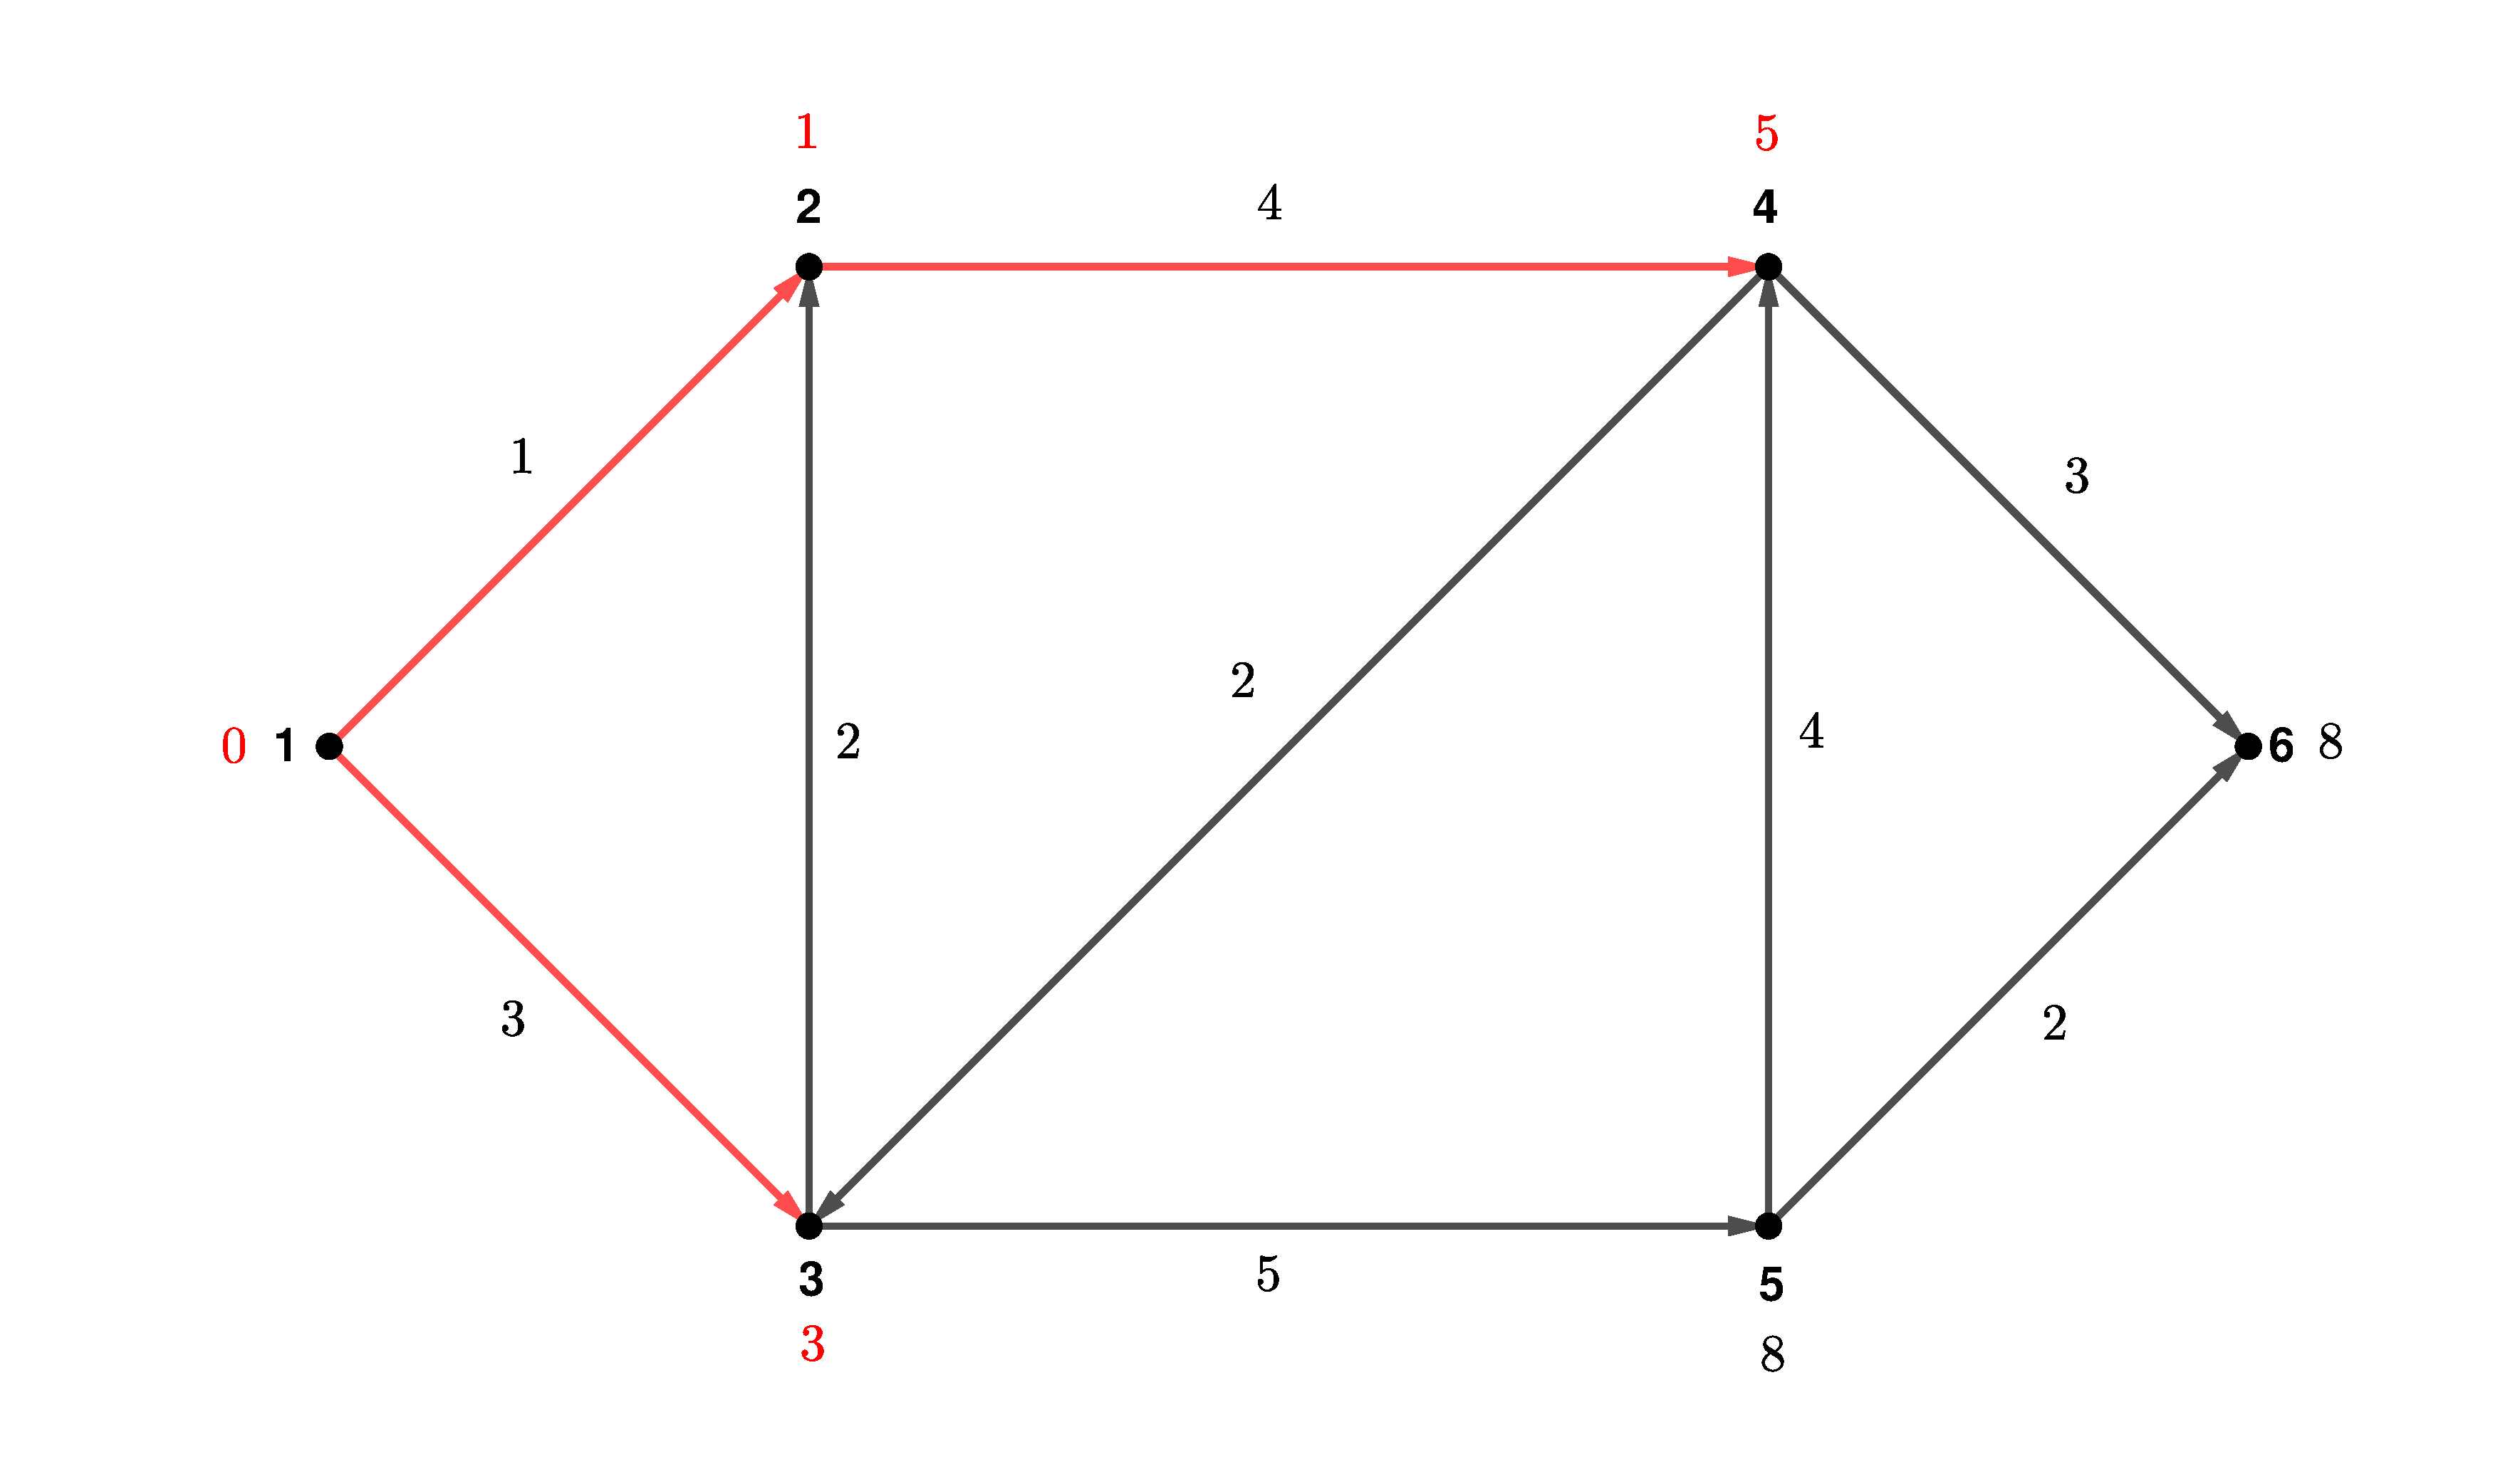
\includegraphics[scale = 0.15]{../图/13.1.5}
	\end{figure}
	
	选择点$5,8$的临时标号为永久标号,因此自点$1$到其他各点的最短有向路为
	\begin{figure}[H]
		\centering
		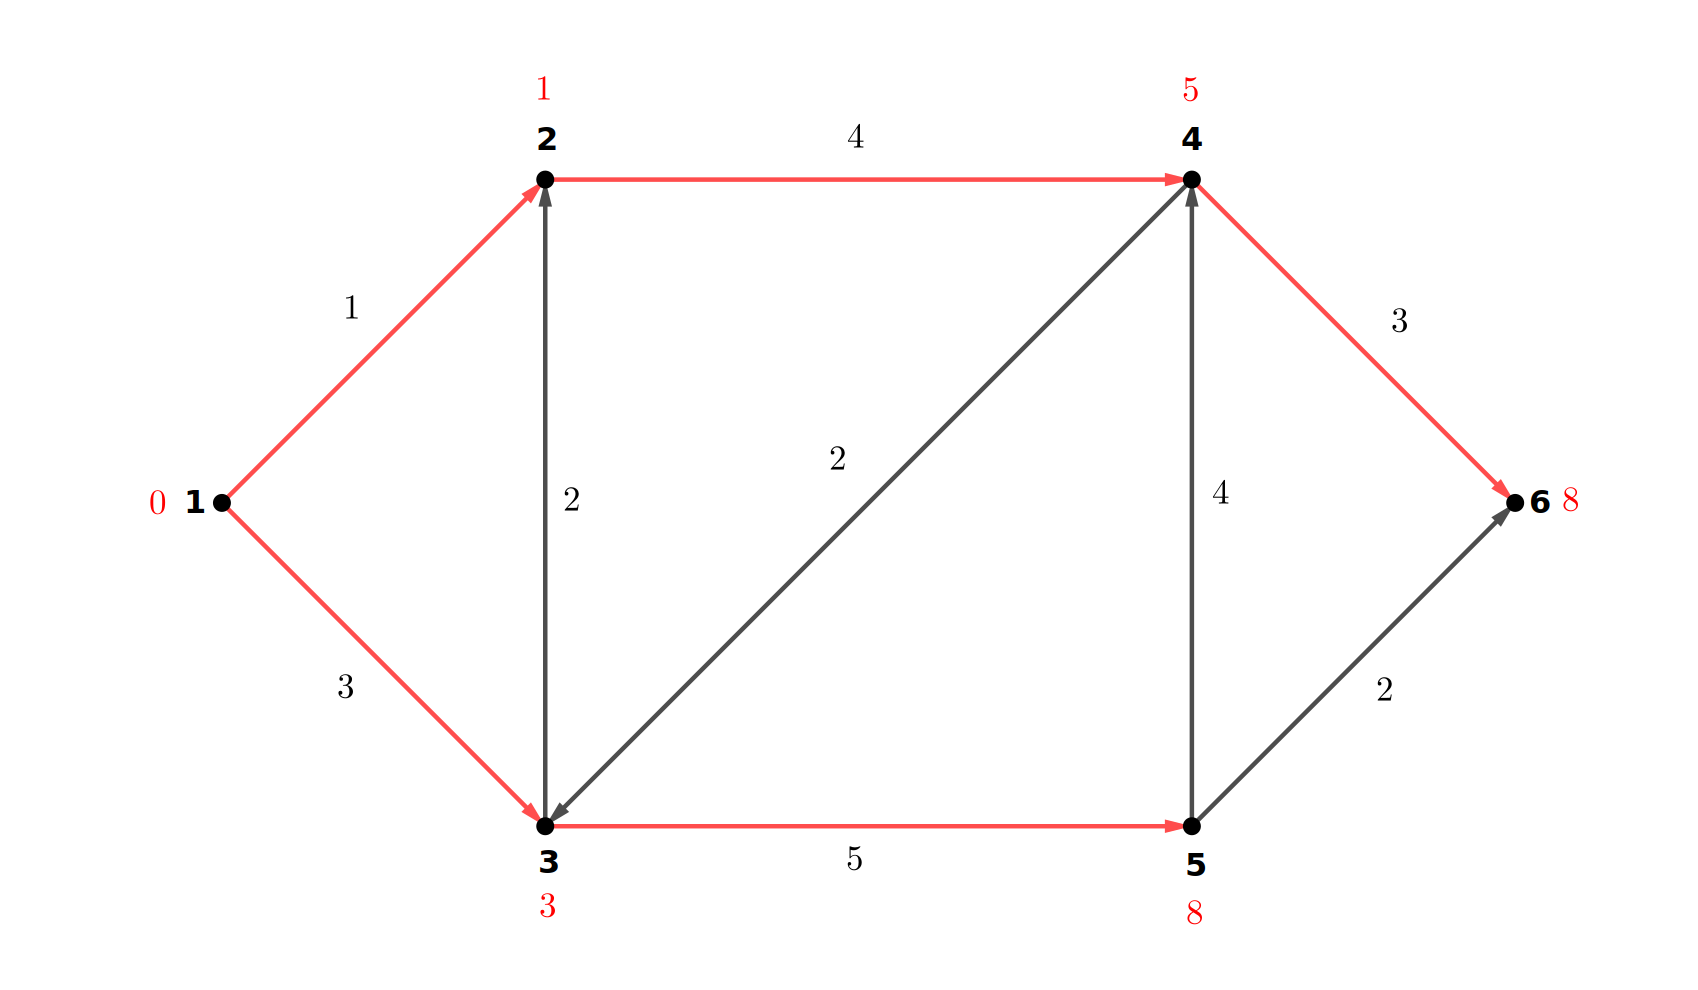
\includegraphics[scale = 0.15]{../图/13.1.6}
	\end{figure}
	\begin{table}[H]
		\centering
		\begin{tabular}{ccc}
			\toprule
			\textbf{城市} & \textbf{最短路线} & \textbf{最短路程} \\
			\midrule
			$2$ & $1\to 2$ & $1$ \\
			$3$ & $1\to 3$ & $3$ \\
			$4$ & $1\to 2\to 4$ & $5$ \\
			$5$ & $1\to 3\to 5$ & $8$ \\
			$6$ & $1\to 2\to 4\to 6$ & $8$ \\
			\bottomrule
		\end{tabular}
	\end{table}
\end{solution}

\section{最大流问题}

\begin{definition}{最大流问题}
	对于有向网络$G=(V,E,C)$,其中$c_{ij}$表示有向边$(i,j)$的容量,令$s$为发点,$t$为收点%
	$$
	x_{ij}=\text{通过有向边}(i,j)\text{的流量}
	$$
	那么求%
	$$
	\max v=
	\max \sum_{j}x_{ij}=
	\max \sum_{j}x_{ji}
	$$
	使得成立
	\begin{align*}
		& 0\le x_{ij}\le c_{ij}\\
		& \sum_{j}x_{ij}-\sum_{j}x_{ji}=\begin{cases}
			+v,\qquad & i=s\\
			-v,\qquad & i=t\\
			0,\qquad & \text{其他}
		\end{cases}
	\end{align*}
\end{definition}

\begin{theorem}{最大流算法}
	\begin{enumerate}
		\item 令$x=(x_{ij})$为整数可行流,可以为零流,给$s$一个永久标号$(-,\infty)$。
		\item \begin{enumerate}
			\item 如果所有标号点的相邻点均已检查,转至第4步。
			\item 找一个已标号但存在未检查的相邻点的点$i$,对于每一个有向边$(i,j)$,若$x_{ij}<c_{ij}$且$j$未标号,则给$j$一个标号$(+i,\delta(j))$,其中%
			$$
			\delta(j)=\min\{ c_{ij}-x_{ij},\delta(i) \}
			$$
			对于每一个有向边$(j,i)$,若$x_{ji}>0$且$j$未标号,则给$j$一个标号$(-i,\delta(j))$,其中%
			$$
			\delta(j)=\min\{ x_{ji},\delta(i) \}
			$$
			\item 若$t$已被标号,转至第3步,否则转至2.a。
		\end{enumerate}
		\item 由点$t$开始,使用指示标号构造一个增广路,指示标号的正负表示通过增加还是减少流量来增大流值。删去点$s$以外的所有标号,转至第2步。
		\item 此时现行流是最大的,若把所有标号点的集合记为$S$,所有未标号的点的集合记为$T$,便得到最小容量割$(S,T)$,计算完成。
	\end{enumerate}
\end{theorem}

\begin{example}
	使用Ford-Fulkerson算法求如下图所示的有向网络中从$s$到$t$的最大流。
	\begin{figure}[H]
		\centering
		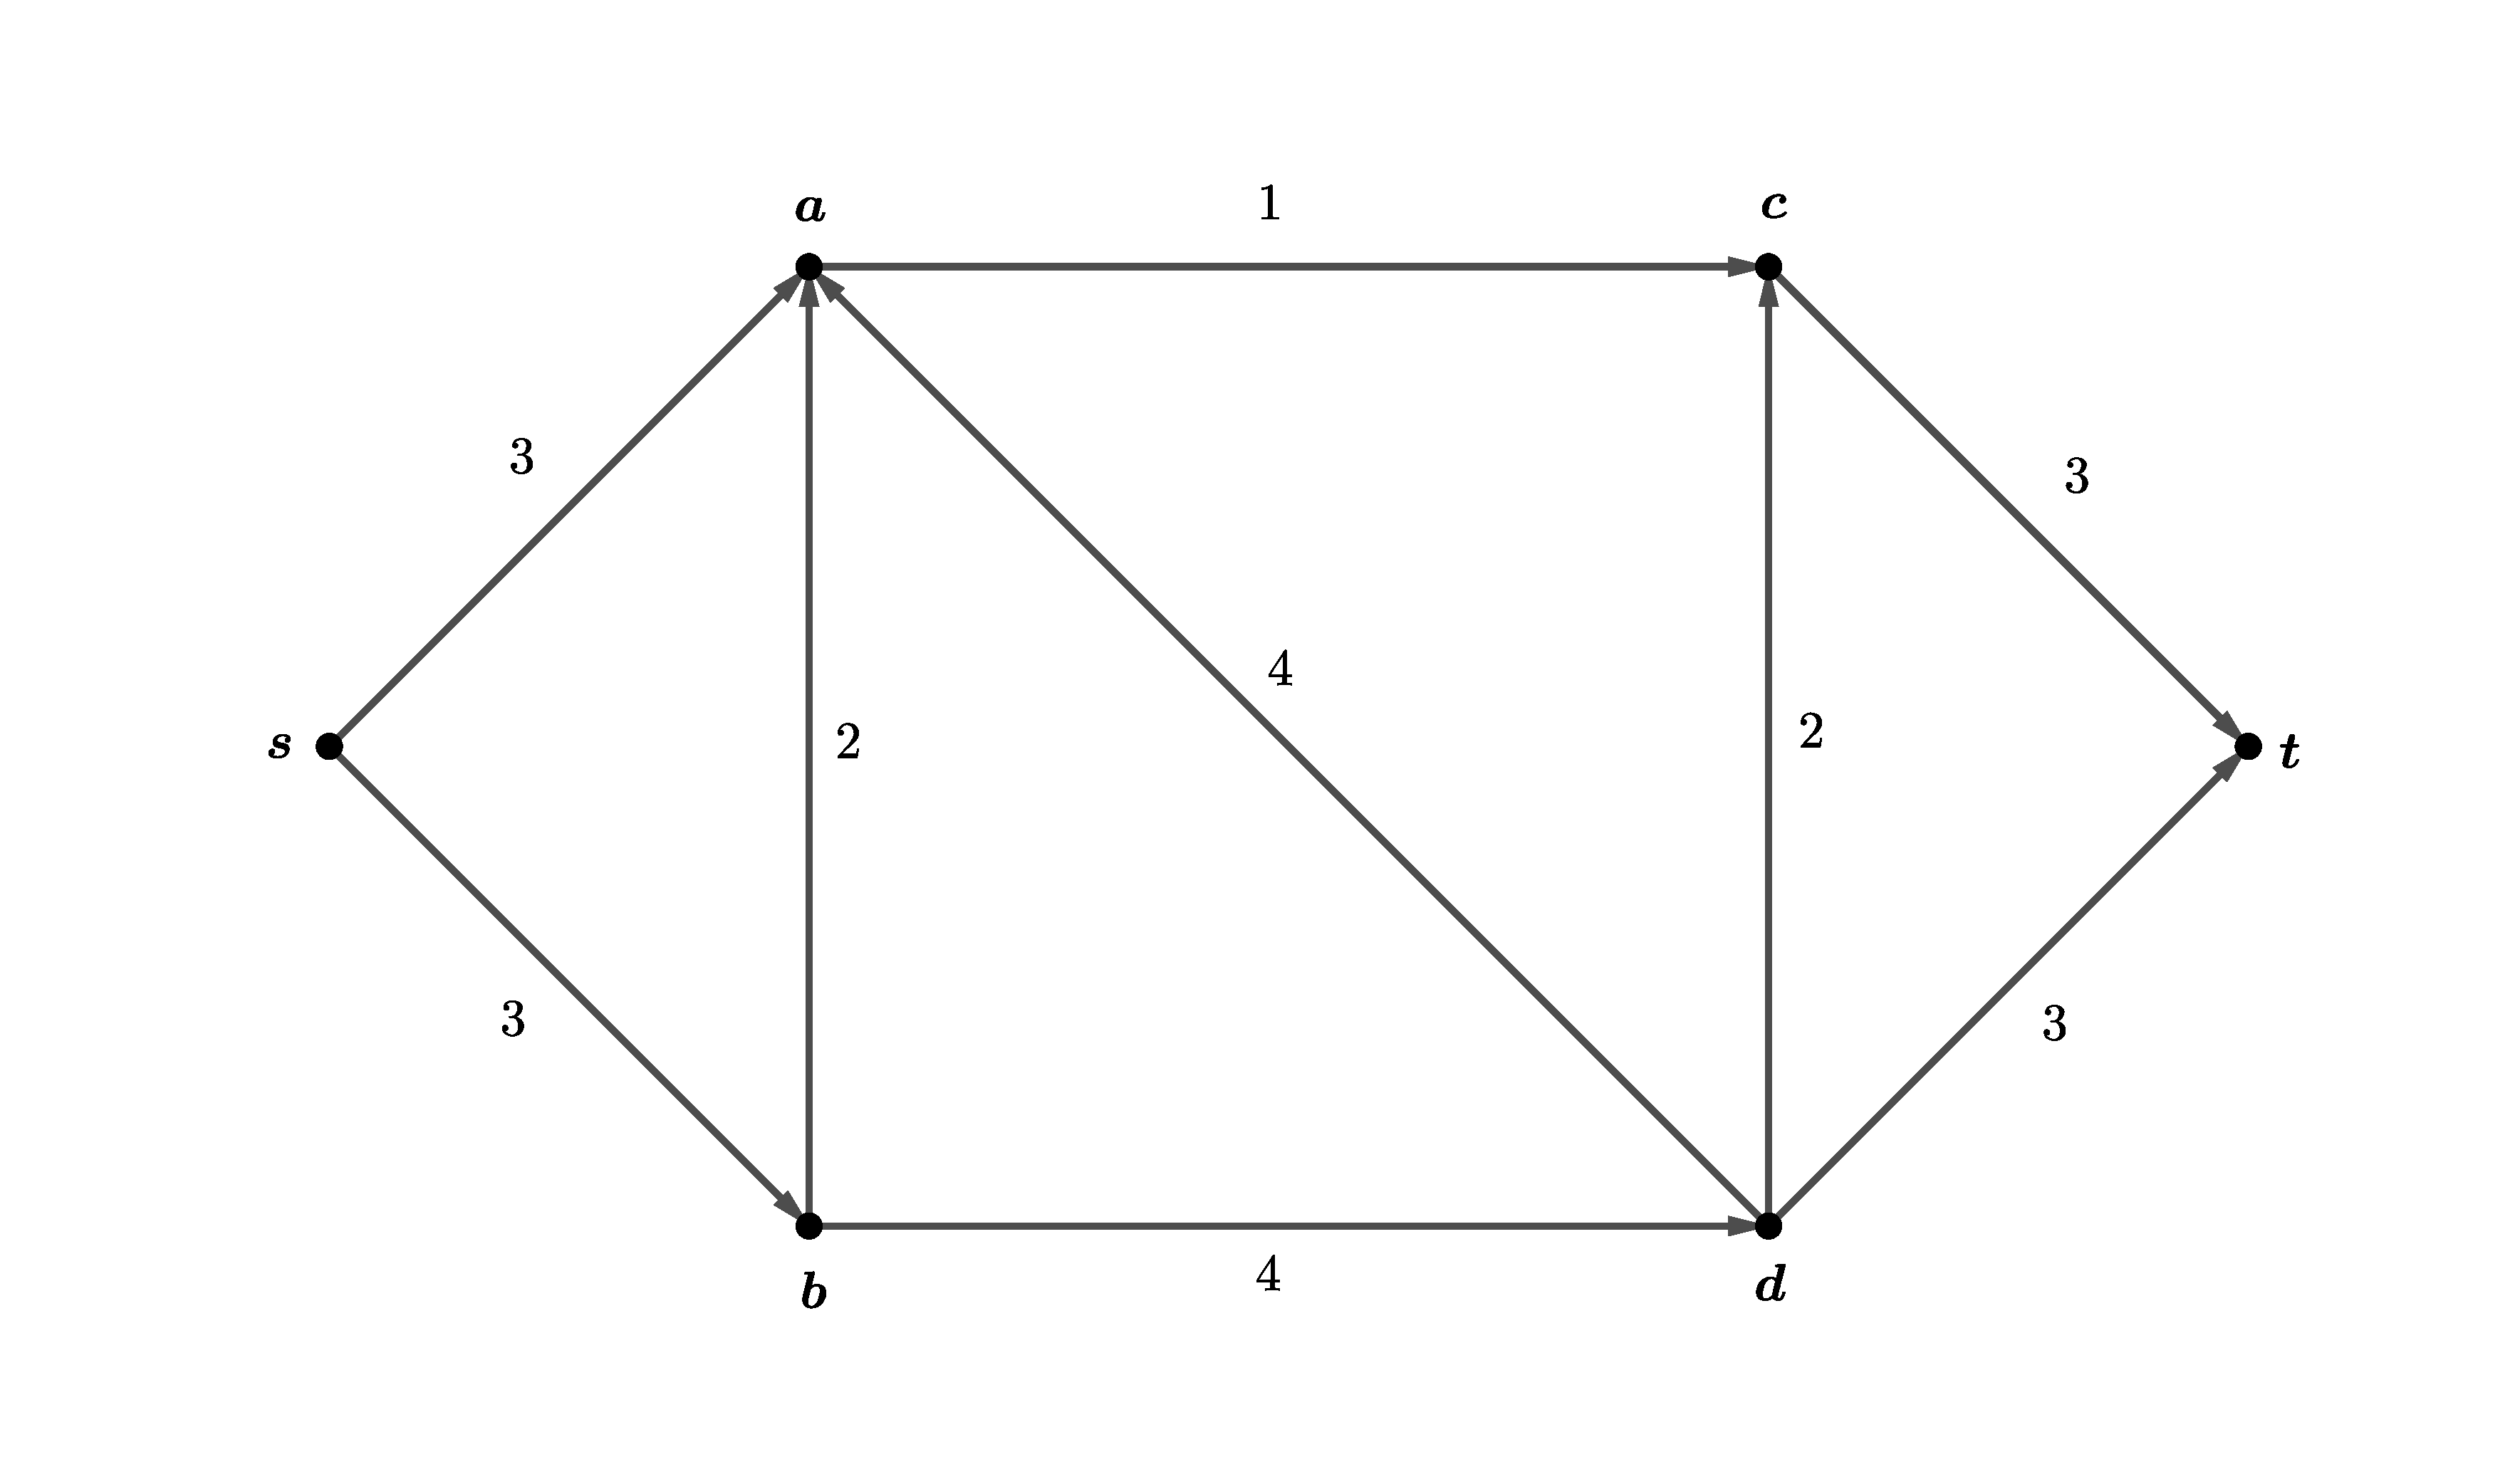
\includegraphics[scale = 0.15]{../图/13.2.1}
	\end{figure}
\end{example}

\begin{solution}
	作零流
	\begin{figure}[H]
		\centering
		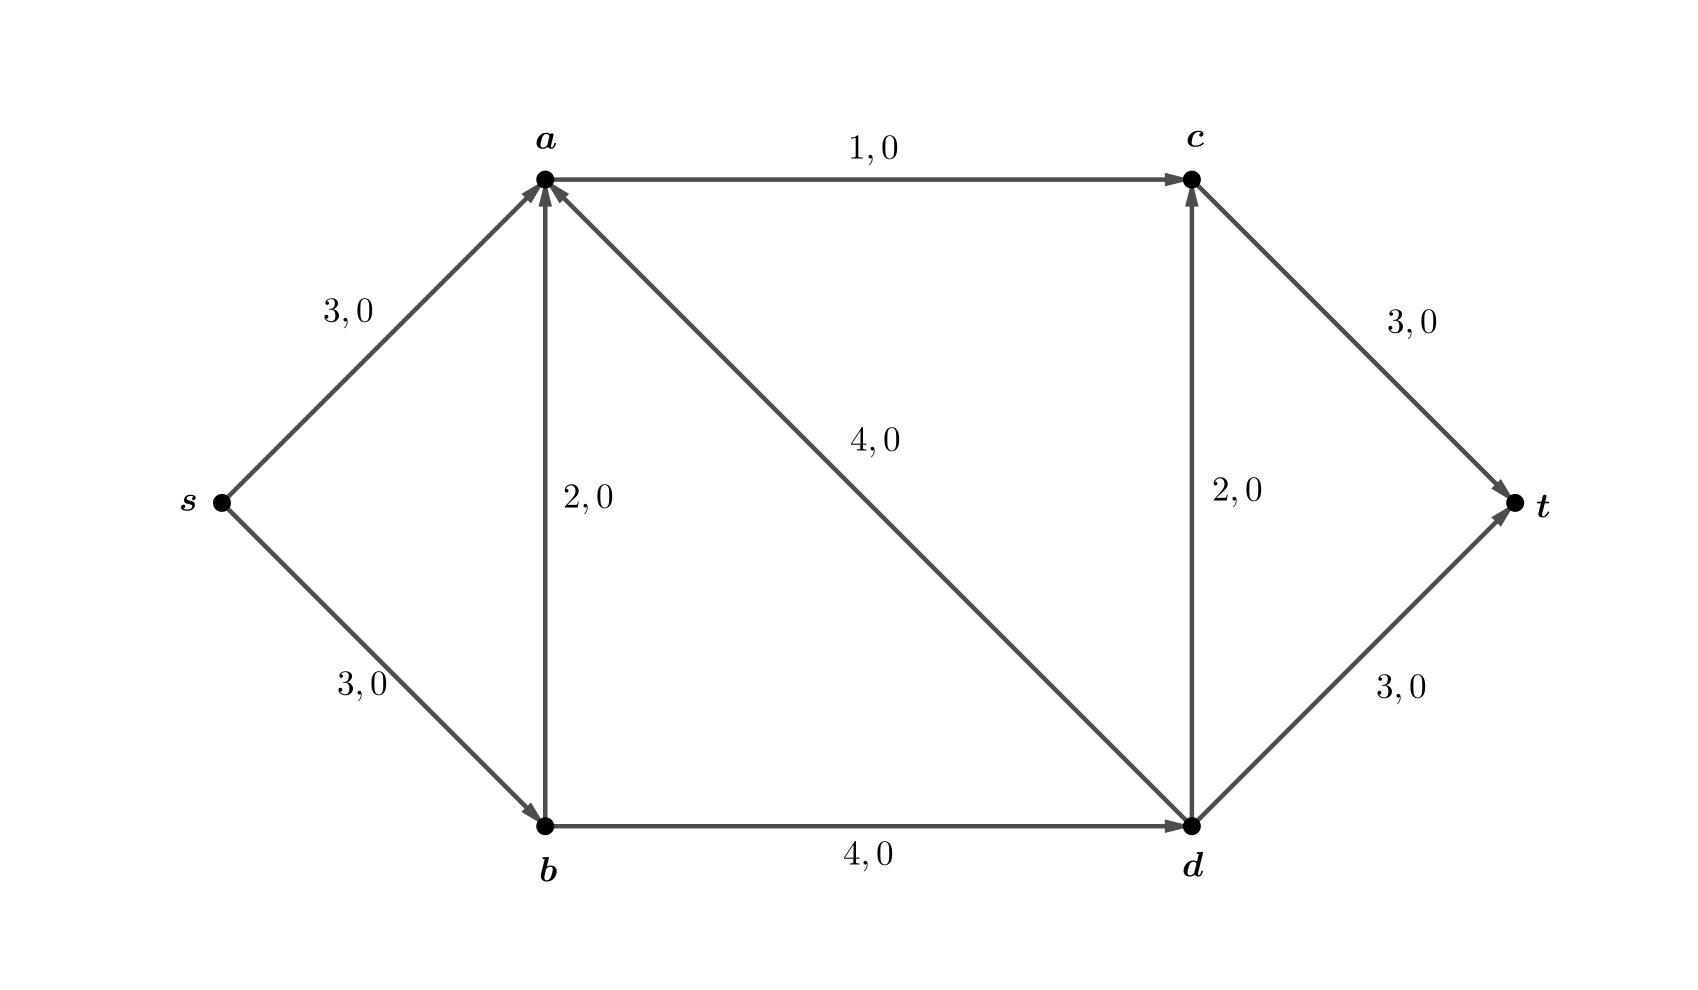
\includegraphics[scale = 0.15]{../图/13.2.2}
	\end{figure}
	
	依次标号
	\begin{figure}[H]
		\centering
		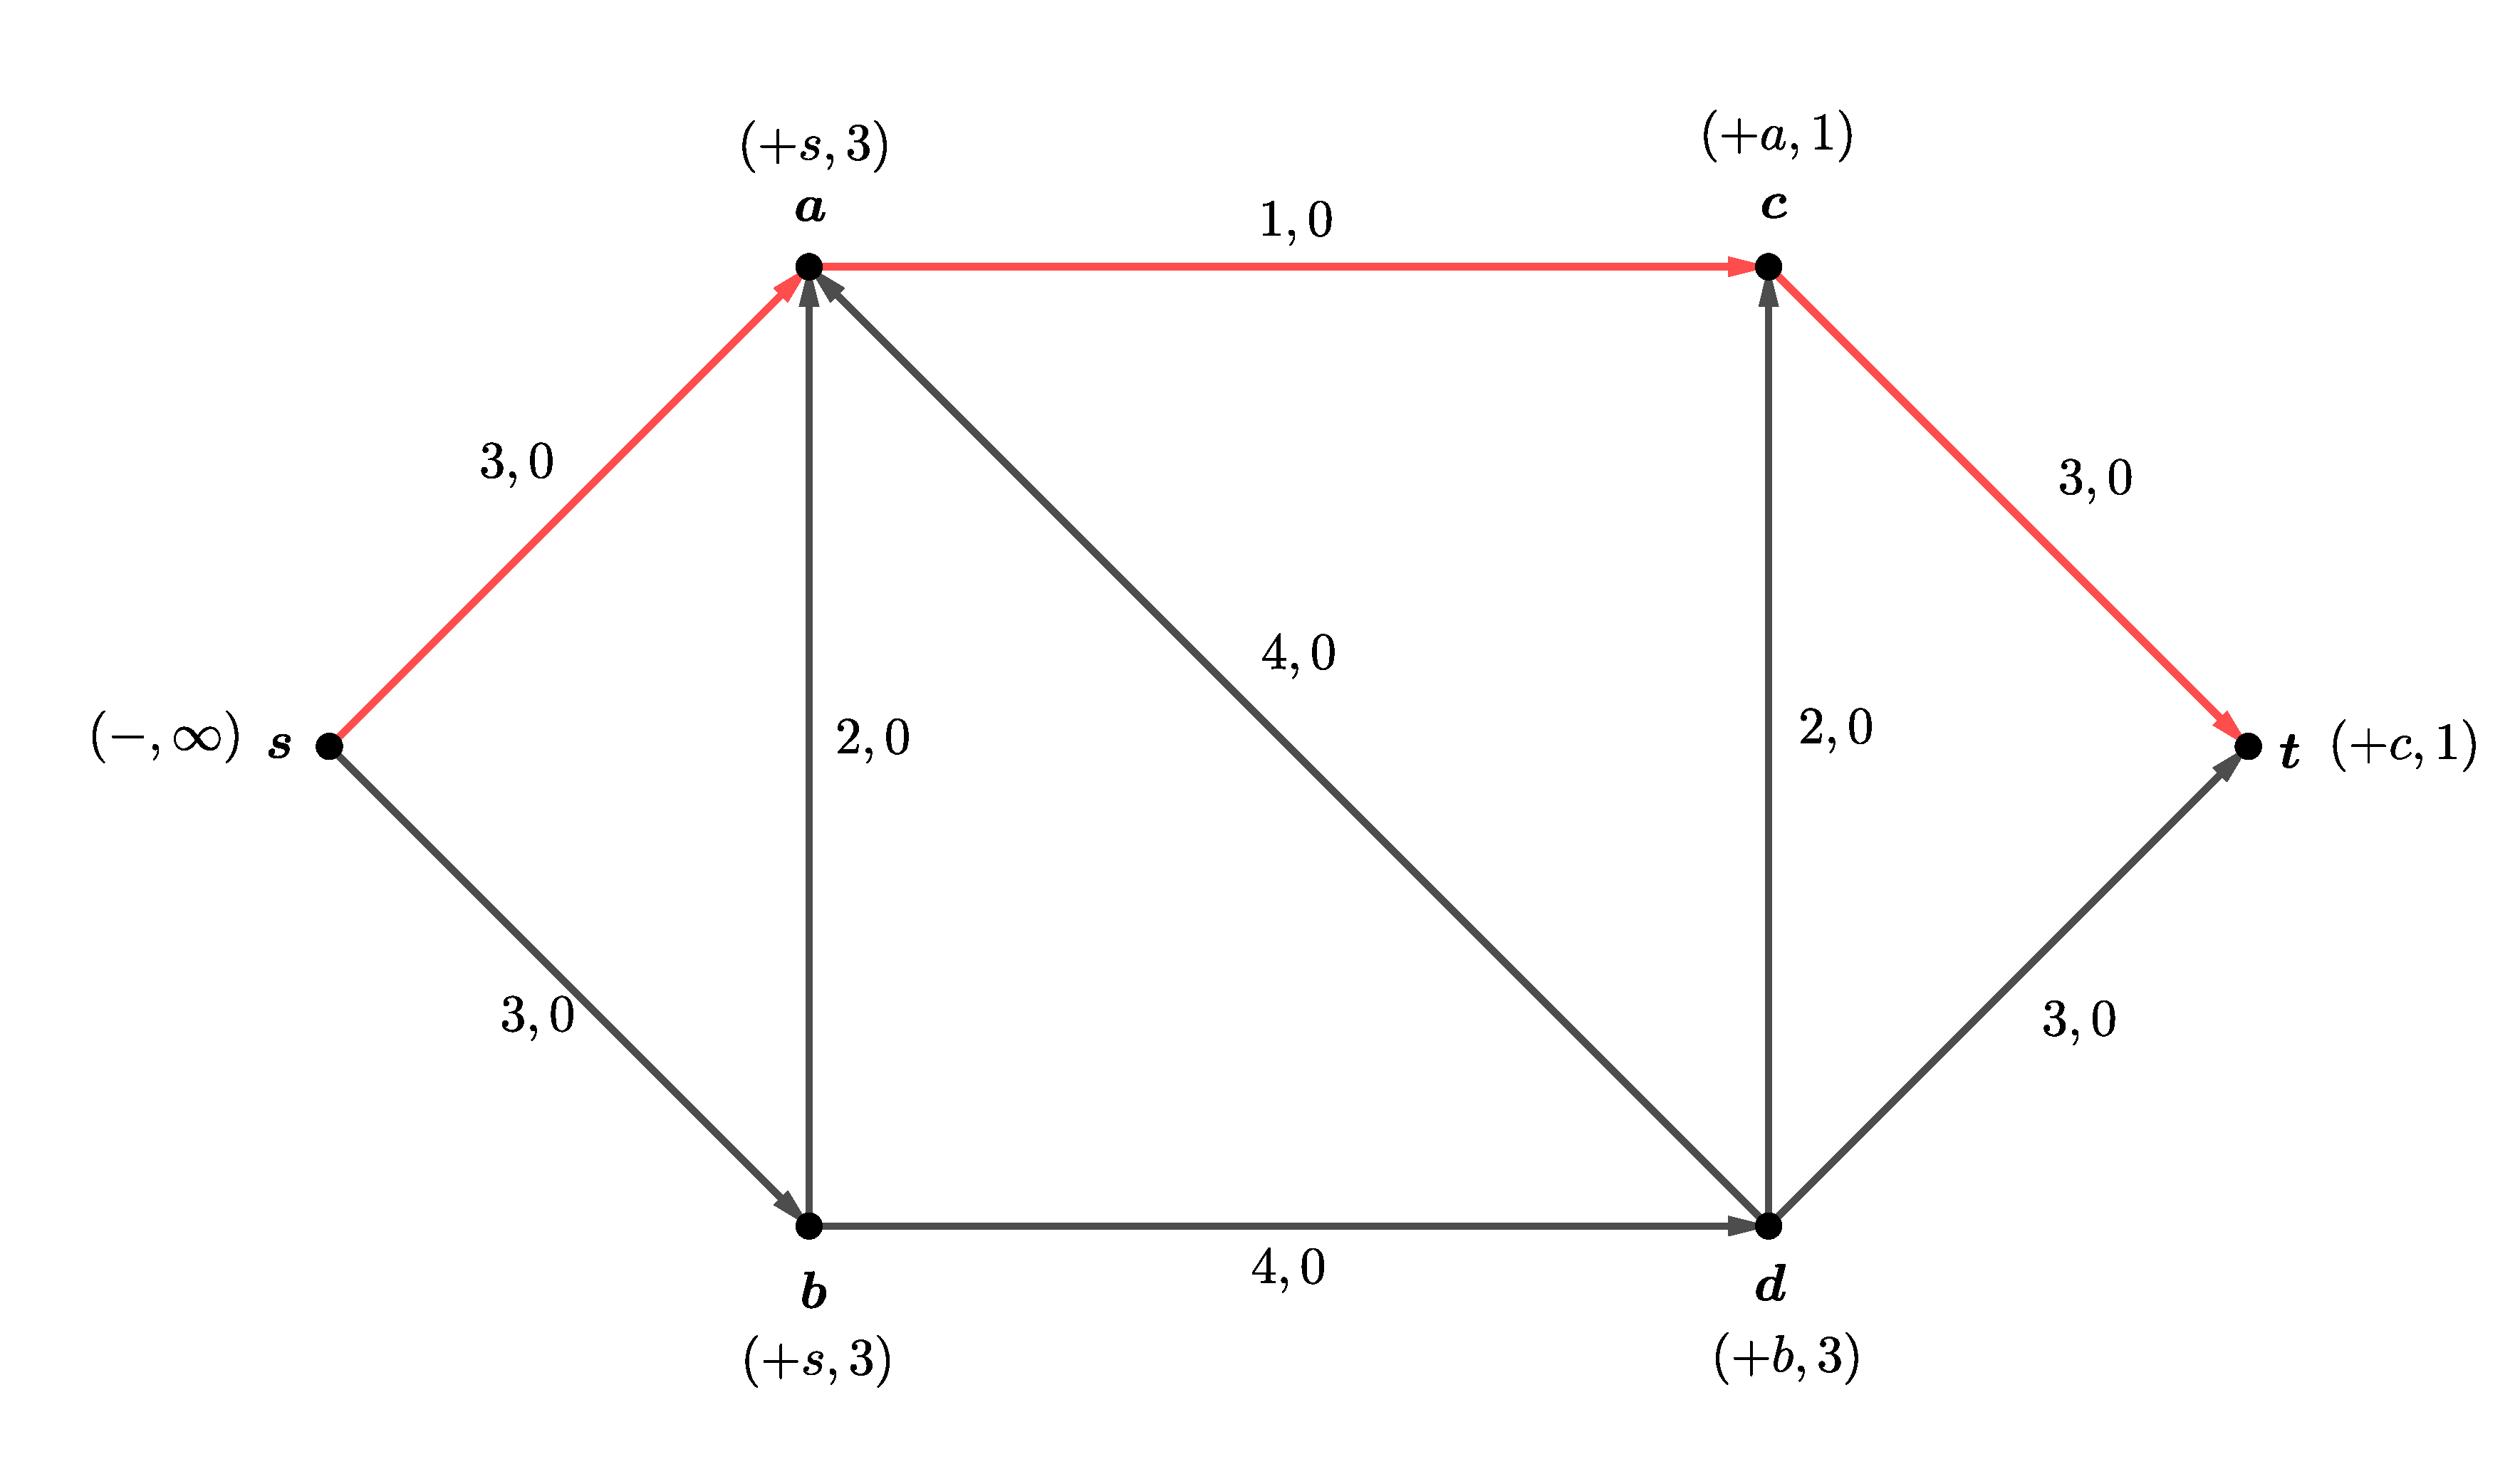
\includegraphics[scale = 0.15]{../图/13.2.3}
	\end{figure}
	更新流量
	\begin{figure}[H]
		\centering
		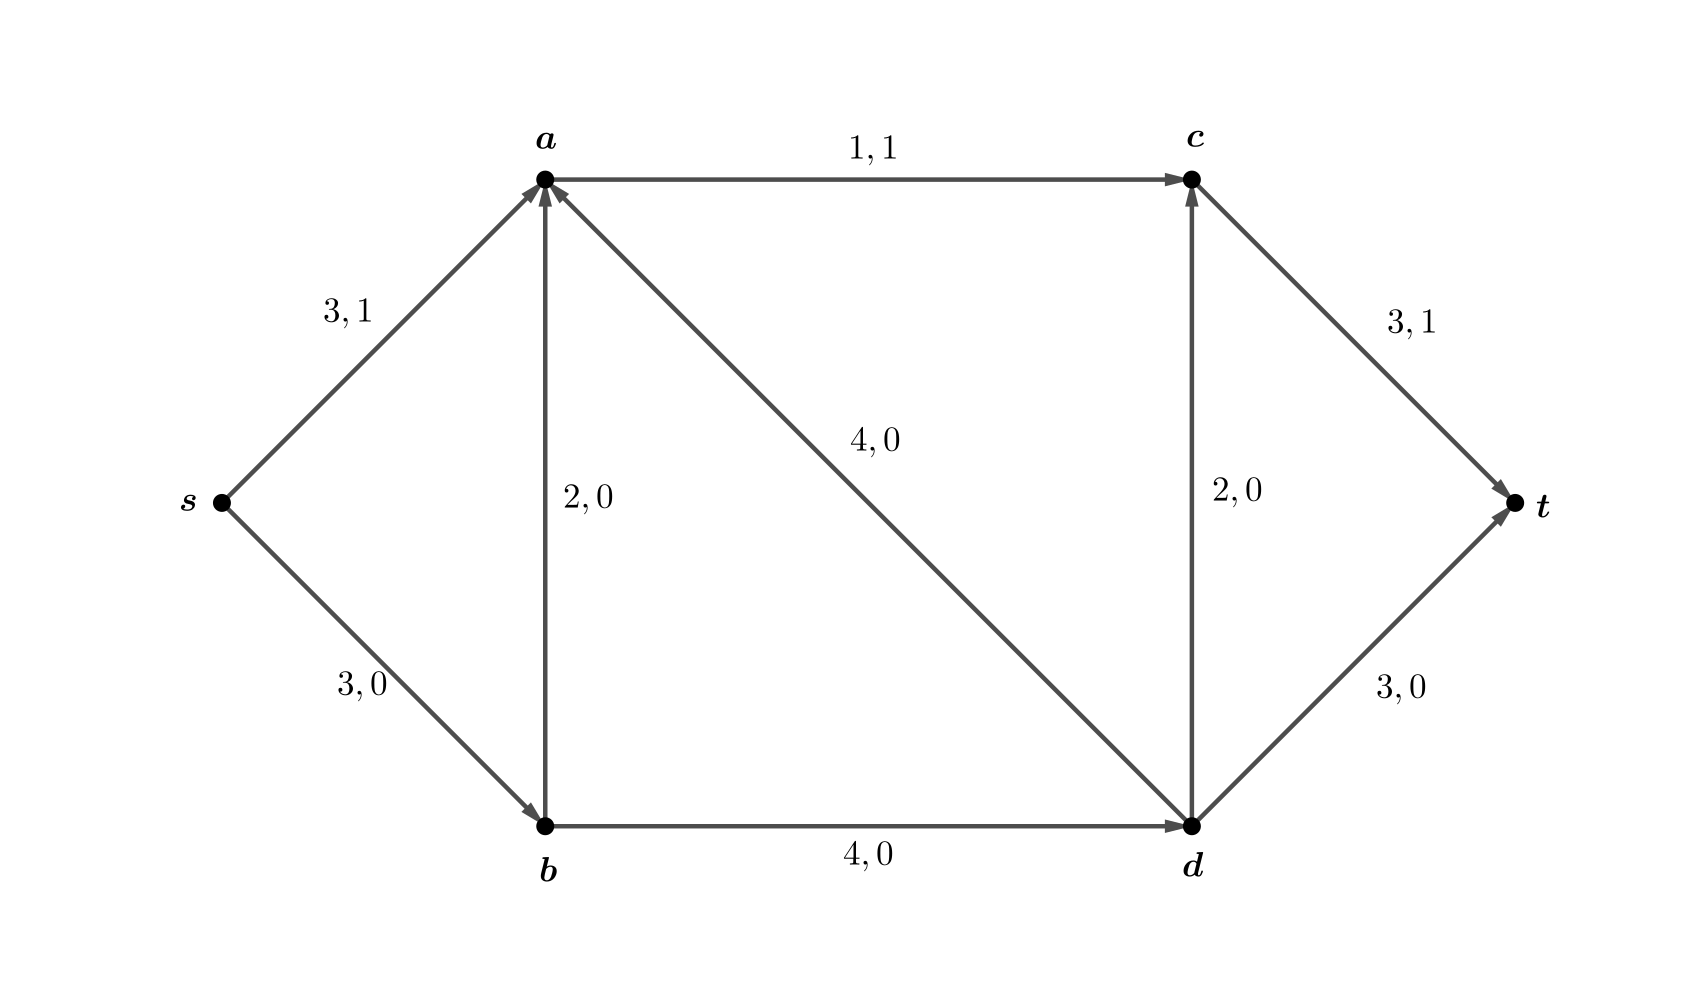
\includegraphics[scale = 0.15]{../图/13.2.4}
	\end{figure}
	
	依次标号
	\begin{figure}[H]
		\centering
		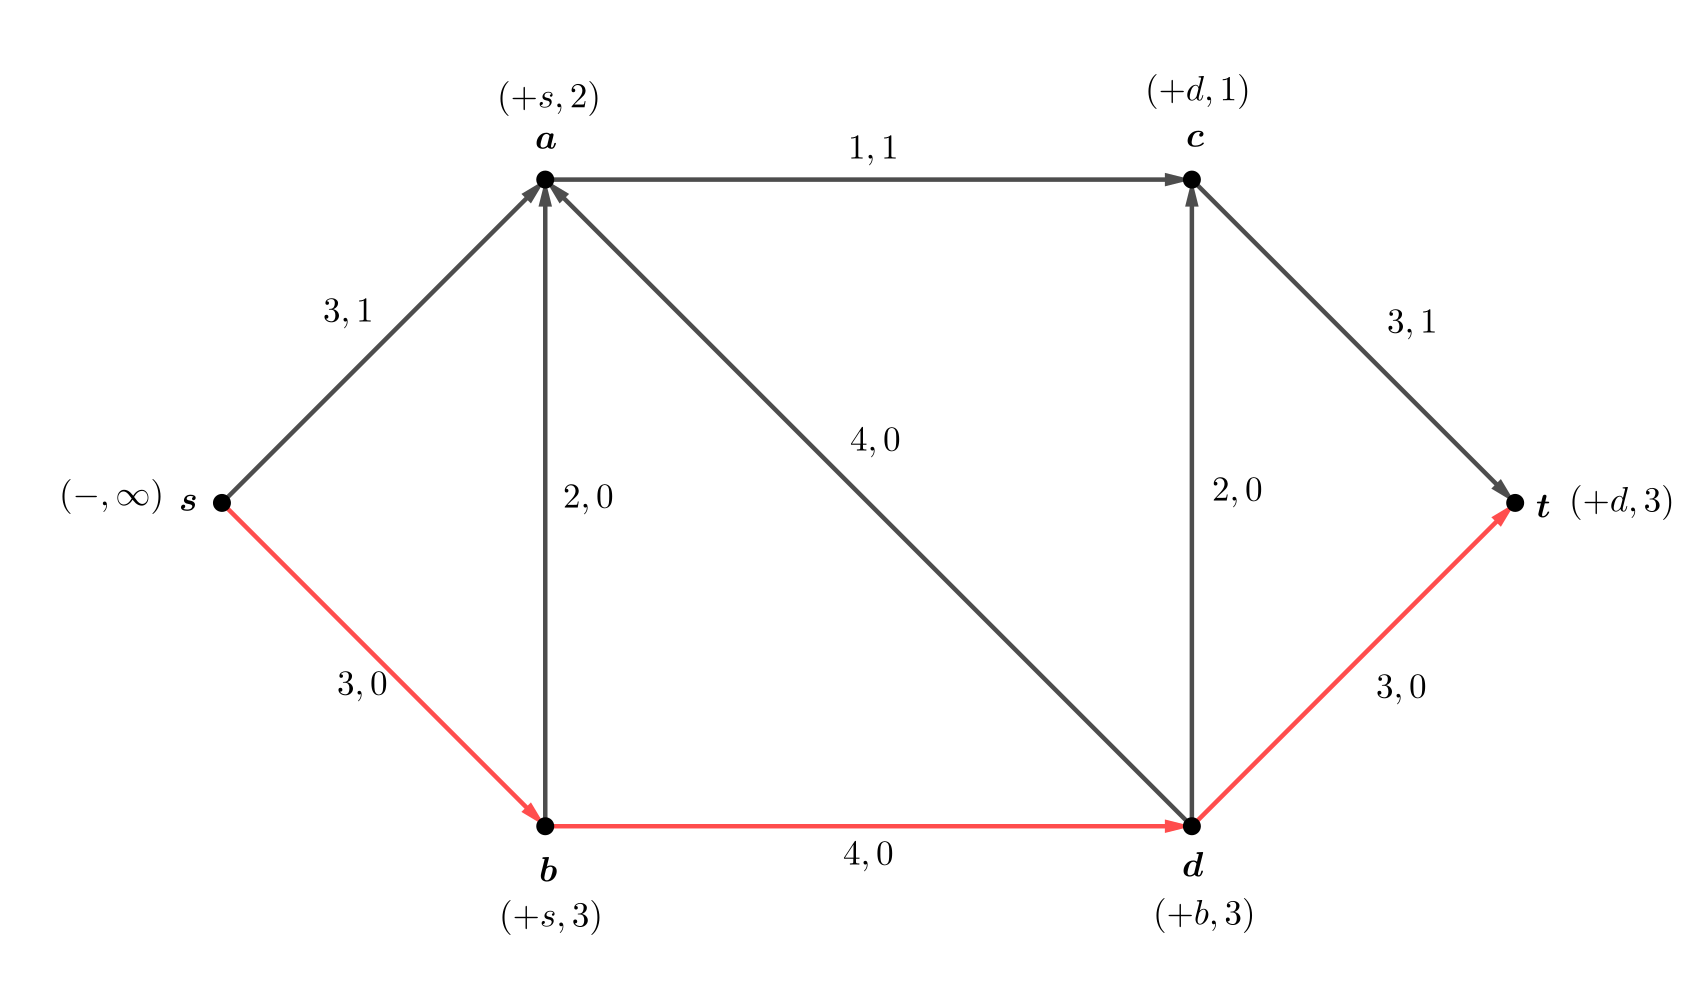
\includegraphics[scale = 0.15]{../图/13.2.5}
	\end{figure}
	更新流量
	\begin{figure}[H]
		\centering
		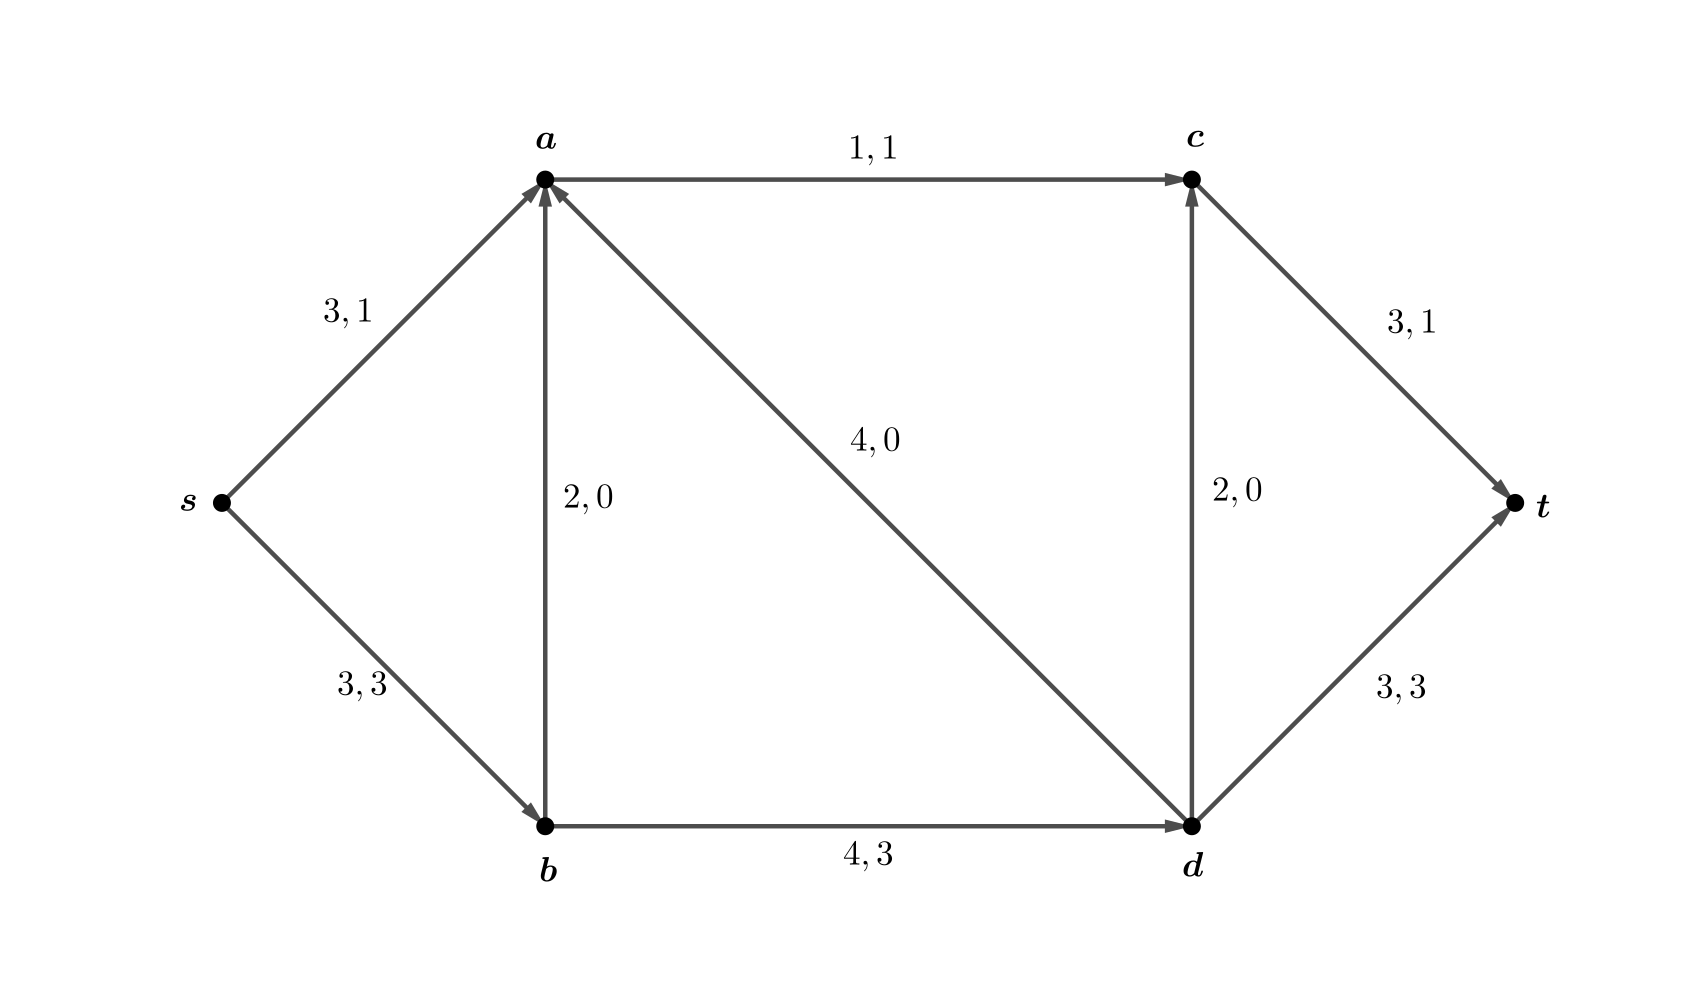
\includegraphics[scale = 0.15]{../图/13.2.6}
	\end{figure}
	
	依次标号
	\begin{figure}[H]
		\centering
		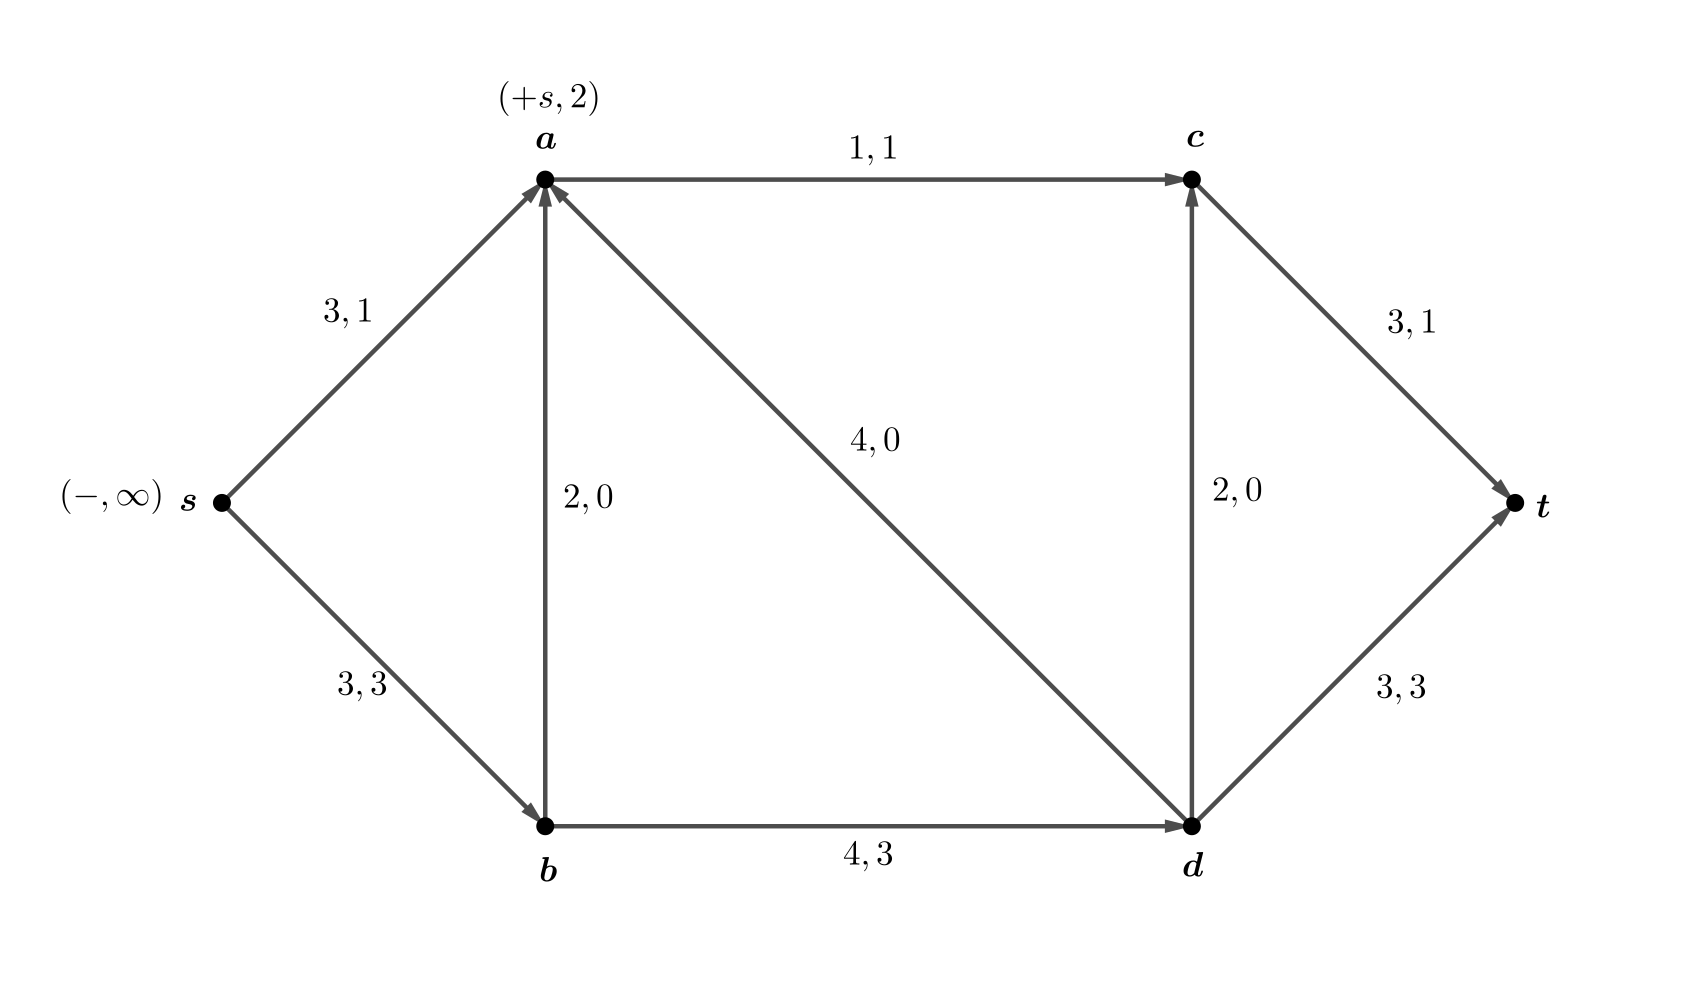
\includegraphics[scale = 0.15]{../图/13.2.7}
	\end{figure}
	
	此时流量最大,流量如下
	\begin{table}[H]
		\centering
		\begin{tabular}{c|ccccccc}
			\hline
			边 & $(s,a)$ & $(s,b)$ & $(a,c)$ & $(b,d)$ & $(c,t)$ & $(d,t)$ & 其他 \\
			\hline
			流量 & $1$ & $3$ & $1$ & $3$ & $1$ & $3$ & $0$ \\ \hline
		\end{tabular}
	\end{table}	
	最大流为$v=4$。
\end{solution}

\chapter{排队论}

\section{基本模型}

\textbf{基本组成部分:}

\begin{enumerate}
	\item 输入过程:顾客按照怎样的规律到达。
	\begin{enumerate}
		\item 顾客来源
		\begin{enumerate}
			\item 有限
			\item 无限
		\end{enumerate}
		\item 顾客数量
		\begin{enumerate}
			\item 有限
			\item 无限
		\end{enumerate}
		\item 经常性的顾客来源
		\begin{enumerate}
			\item 顾客到达间隔时间:到下一个顾客到达的时间。
			\item 服从某一频率分别(指数分布)。
		\end{enumerate}
		\item 顾客的行为假定
		\begin{enumerate}
			\item 在未服务之间不会离开。
			\item 当看到队列很长的时候离开。
			\item 从一个队列移到另一个队列。
		\end{enumerate}
	\end{enumerate}
	\item 排队规则:顾客按照一定规则排队等待服务。
	\item 服务机构:服务机构的设置,服务台的数列,服务的方式,服务时间分布等。
\end{enumerate}

\textbf{记号方案:}
\begin{enumerate}
	\item $M$:指数分布
	\item $D$:定长分布
	\item $E_k$:$k$级Erlang分布
\end{enumerate}

\begin{definition}{负指数分布}
	对于参数为$1/\lambda$的指数分布$\xi$,其分布密度函数为%
	$$
	f(t)=\begin{cases}
		\lambda\ee{-\lambda t},\qquad & t\ge 0\\
		0,\qquad & t<0
	\end{cases}
	$$
	分布函数为
	$$
	F(t)=\begin{cases}
		1-\ee{-\lambda t},\qquad & t\ge 0\\
		0,\qquad & t<0
	\end{cases}
	$$
	数学期望与方差为%
	$$
	E(\xi)=\frac{1}{\lambda},\qquad
	D(\xi)=\frac{1}{\lambda^2}
	$$
\end{definition}

\begin{theorem}{指数分布的无记忆性}
	$$
	P\{ \xi>t+x\mid \xi>t \}
	=P\{ \xi>x \}
	$$
\end{theorem}

\begin{definition}{最简单流}
	称事件流$N(t)$为最简单流,如果满足如下性质。
	\begin{enumerate}
		\item 平稳性:对于任意时刻$t_0$,$(t_0,t_0+t]$时间内出现的事件数仅与事件长度$t$有关,而与起点$t_0$无关。
		\item 无记忆性:$(t_0,t_0+t]$时间内出现$k$个事件与时刻$t_0$以前出现的事件数无关。
		\item 普通性:在充分小的时间区间$\Delta t$内,发生两个及两个以上事件的概率为比$\Delta t$高阶的无穷小量。
	\end{enumerate}
\end{definition}

\section{$M/M/1/\infty$模型}

$\lambda$:单位时间内平均到达的顾客人数。

$\mu$:单位时间平均服务完的顾客人数。

$\rho=\lambda/\mu$:服务强度。

$N(t)$表示$t$时刻在系统中的顾客数量,其概率公式为
$$
p_n
=P\{ N(t)=n \}
=(1-\rho)\rho^n
$$
$N_q(t)=N(t)-1$表示$t$时刻在系统中的排队等待的顾客数量。

\textbf{在系统中的平均顾客数量},换言之,\textbf{平均队长}为
$$
L
=E(N)
=\sum_{n=0}^{\infty}np_n
=\sum_{n=0}^{\infty}n(1-\rho)\rho^n
=\frac{\rho}{1-\rho}
$$

\textbf{在系统中的平均排队等待的顾客数量}为
$$
L_q
=E(N_q)
=\sum_{n=1}^{\infty}(n-1)p_n
=\sum_{n=1}^{\infty}(n-1)(1-\rho)\rho^n
=\frac{\rho^2}{1-\rho}
$$

\textbf{平均逗留时长}为
$$
W=W_q+\frac{1}{\mu}
=\frac{1}{\mu-\lambda}
$$

\textbf{平均等待时长}为
$$
W_q
=\sum_{n=0}^{\infty}\frac{n}{\mu}p_n
=\frac{1}{\mu}E(N)
=\frac{\rho}{\mu-\lambda}
=\frac{\lambda}{\mu(\mu-\lambda)}
$$

\chapter{决策分析}

\section{模型建立}

决策问题的基本要素:
\begin{enumerate}
	\item 状态集$S=\{ x \}$:把决策的对象统称为一个系统,系统处于不同的状况称为状态。
	\item 决策集$A=\{ a \}$:为达到预想的目标提出的每一个行动方案称为决策方案。
	\item 报酬函数$R(a,x)$:在状态$x$出现时,决策者采取方案$a$所得到收益值。
\end{enumerate}

\section{风险型决策分析}

\section{不确定型决策分析}

\textbf{乐观法}:%
$$
\Phi:\qquad\max_{a\in A}\{ \max_{x\in S}\{ R(a,x) \} \}
$$

\textbf{悲观法}:%
$$
\Phi:\qquad\max_{a\in A}\{ \min_{x\in S}\{ R(a,x) \} \}
$$

\textbf{乐观系数法}:%
$$
\Phi:\qquad\max_{a\in A}\{ \alpha\max_{x\in S}\{ R(a,x) \}+(1-\alpha)\min_{x\in S}\{ R(a,x) \} \}
$$

\textbf{等可能法}:%
$$
\Phi:\qquad\max_{a\in A}\left\{ \frac{1}{n}\sum_{k=1}^{n}R(a,x_k) \right\}
$$

\textbf{后悔值法}:
\begin{align*}
	& \text{RV}(a,x)=\max_{a\in A}\{ R(a,x) \}-R(a,x)\\
	& \Phi:\qquad \min_{a\in A}\{ \max_{x\in S}\{ \text{RV}(a,x) \} \}
\end{align*}

\begin{example}
	某公司欲购进一种新产品,有三种可供选择的方案,即大批量购进、中批量购进、小批量购进,在各种市场需要下推销该产品的获利情况如下表所示,其中负数表示亏损。
	\begin{table}[H]
		\centering
		\caption{获利情况}
		\renewcommand{\arraystretch}{1.5}
		\begin{tabular}{|>{\centering\arraybackslash}m{2cm}>{\centering\arraybackslash}m{2.5cm}|>{\centering\arraybackslash}m{1.5cm}>{\centering\arraybackslash}m{1.5cm}>{\centering\arraybackslash}m{1.5cm}|}
			\hline
			\multicolumn{2}{|c|}{\multirow{2}{*}{利润/万元}}      & \multicolumn{3}{c|}{市场情况} \\ \cline{3-5} 
			\multicolumn{2}{|c|}{}                            & 畅销      & 一般     & 滞销     \\ \hline
			\multicolumn{1}{|c|}{\multirow{3}{*}{方案}} & 大批量购进 & $600$     & $200$    & $-80$    \\
			\multicolumn{1}{|c|}{}                    & 中批量购进 & $400$     & $300$    & $-20$    \\
			\multicolumn{1}{|c|}{}                    & 小批量购进 & $200$     & $100$    & $-10$    \\ \hline
		\end{tabular}
	\end{table}
	分别用乐观法、悲观法、乐观系数法(乐观系数$\alpha=0.4$)、后悔值法和等可能法进行决策分析,找出最优方案。
\end{example}

\begin{solution}
	状态集为%
	$$
	S=\{ \text{畅销},\text{一般},\text{滞销} \}
	$$
	决策集为%
	$$
	A=\{ \text{大批量购进},\text{中批量购进},\text{小批量购进} \}
	$$
	决策表为
	\begin{table}[H]
		\centering
		\caption{决策表}
		\renewcommand{\arraystretch}{1.5}
		\begin{tabular}{|>{\centering\arraybackslash}m{2cm}>{\centering\arraybackslash}m{3cm}|>{\centering\arraybackslash}m{2cm}>{\centering\arraybackslash}m{2cm}>{\centering\arraybackslash}m{2cm}|}
			\hline
			\multicolumn{2}{|c|}{\multirow{2}{*}{$R(a,x)$/万元}}      & \multicolumn{3}{c|}{市场情况} \\ \cline{3-5} 
			\multicolumn{2}{|c|}{}                            & $x_1$(畅销)      & $x_2$(一般)     & $x_3$(滞销)     \\ \hline
			\multicolumn{1}{|c|}{\multirow{3}{*}{方案}} & $a_1$(大批量购进) & $600$     & $200$    & $-80$    \\
			\multicolumn{1}{|c|}{}                    & $a_2$(中批量购进) & $400$     & $300$    & $-20$    \\
			\multicolumn{1}{|c|}{}                    & $a_3$(小批量购进) & $200$     & $100$    & $-10$    \\ \hline
		\end{tabular}
	\end{table}
	\begin{enumerate}
		\item 对于乐观法,乐观法决策表为
		\begin{table}[H]
			\centering
			\caption{乐观法决策表}
			\renewcommand{\arraystretch}{1.5}
			\begin{tabular}{|>{\centering\arraybackslash}m{2cm}>{\centering\arraybackslash}m{3cm}|>{\centering\arraybackslash}m{2cm}>{\centering\arraybackslash}m{2cm}>{\centering\arraybackslash}m{2cm}|>{\centering\arraybackslash}m{2.5cm}|}
				\hline
				\multicolumn{2}{|c|}{\multirow{2}{*}{$R(a,x)$/万元}}      & \multicolumn{3}{c|}{市场情况} & \multirow{2}{*}{$\dis\max_{x\in S}\{ R(a,x) \}$} \\ \cline{3-5}
				\multicolumn{2}{|c|}{}                            & $x_1$(畅销)      & $x_2$(一般)     & $x_3$(滞销)     &                      \\ \hline
				\multicolumn{1}{|c|}{\multirow{3}{*}{方案}} & $a_1$(大批量购进) & $600$     & $200$    & $-80$    & $600$                   \\
				\multicolumn{1}{|c|}{}                    & $a_2$(中批量购进) & $400$     & $300$    & $-20$    & $400$                 \\
				\multicolumn{1}{|c|}{}                    & $a_3$(小批量购进) & $200$     & $100$    & $-10$    & $200$                 \\ \hline
			\end{tabular}
		\end{table}
		由于
		\begin{align*}
			\Phi:\qquad
			& \max_{a\in A}\{ \max_{x\in S}\{ R(a,x) \} \}\\
			= & \max\{ R(a_1,x_1),R(a_2,x_1),R(a_3,x_1) \}\\
			= & R(a_1,x_1)\\
			= & 600
		\end{align*}
		因此最优方案为大批量购进。
		\item 对于悲观法,悲观法决策表为
		\begin{table}[H]
			\centering
			\caption{悲观法决策表}
			\renewcommand{\arraystretch}{1.5}
			\begin{tabular}{|>{\centering\arraybackslash}m{2cm}>{\centering\arraybackslash}m{3cm}|>{\centering\arraybackslash}m{2cm}>{\centering\arraybackslash}m{2cm}>{\centering\arraybackslash}m{2cm}|>{\centering\arraybackslash}m{2.5cm}|}
				\hline
				\multicolumn{2}{|c|}{\multirow{2}{*}{$R(a,x)$/万元}}      & \multicolumn{3}{c|}{市场情况} & \multirow{2}{*}{$\dis\min_{x\in S}\{ R(a,x) \}$} \\ \cline{3-5}
				\multicolumn{2}{|c|}{}                            & $x_1$(畅销)      & $x_2$(一般)     & $x_3$(滞销)     &                      \\ \hline
				\multicolumn{1}{|c|}{\multirow{3}{*}{方案}} & $a_1$(大批量购进) & $600$     & $200$    & $-80$    & $-80$                   \\
				\multicolumn{1}{|c|}{}                    & $a_2$(中批量购进) & $400$     & $300$    & $-20$    & $-20$                 \\
				\multicolumn{1}{|c|}{}                    & $a_3$(小批量购进) & $200$     & $100$    & $-10$    & $-10$                 \\ \hline
			\end{tabular}
		\end{table}
		由于
		\begin{align*}
			\Phi:\qquad
			& \max_{a\in A}\{ \min_{x\in S}\{ R(a,x) \} \}\\
			= & \max\{ R(a_1,x_3),R(a_2,x_3),R(a_3,x_3) \}\\
			= & R(a_3,x_3)\\
			= & -10
		\end{align*}
		因此最优方案为小批量购进。
		\item 对于乐观系数法,乐观系数法决策表为
		\begin{table}[H]
			\centering
			\caption{乐观系数法决策表}
			\renewcommand{\arraystretch}{1.5}
			\resizebox{\linewidth}{!}{\begin{tabular}{|>{\centering\arraybackslash}m{2cm}>{\centering\arraybackslash}m{3cm}|>{\centering\arraybackslash}m{2cm}>{\centering\arraybackslash}m{2cm}>{\centering\arraybackslash}m{2cm}|>{\centering\arraybackslash}m{6cm}|}
					\hline
					\multicolumn{2}{|c|}{\multirow{2}{*}{$R(a,x)$/万元}}      & \multicolumn{3}{c|}{市场情况} & \multirow{2}{*}{$\dis\alpha\max_{x\in S}\{ R(a,x) \}+(1-\alpha)\min_{x\in S}\{ R(a,x) \}$} \\ \cline{3-5}
					\multicolumn{2}{|c|}{}                            & $x_1$(畅销)      & $x_2$(一般)     & $x_3$(滞销)     &                      \\ \hline
					\multicolumn{1}{|c|}{\multirow{3}{*}{方案}} & $a_1$(大批量购进) & $600$     & $200$    & $-80$    & $192$                   \\
					\multicolumn{1}{|c|}{}                    & $a_2$(中批量购进) & $400$     & $300$    & $-20$    & $148$                 \\
					\multicolumn{1}{|c|}{}                    & $a_3$(小批量购进) & $200$     & $100$    & $-10$    & $74$                 \\ \hline
			\end{tabular}}
		\end{table}
		由于
		\begin{align*}
			\Phi:\qquad
			& \max_{a\in A}\{ \alpha\max_{x\in S}\{ R(a,x) \}+(1-\alpha)\min_{x\in S}\{ R(a,x) \} \}\\
			& \max_{a\in A}\{ 0.4\max_{x\in S}\{ R(a,x) \}+0.6\min_{x\in S}\{ R(a,x) \} \}\\
			= & \max\{ 192,148,74 \}\\
			= & 192
		\end{align*}
		因此最优方案为大批量购进。
		\item 对于后悔值法,后悔值函数为
		$$
		\text{RV}(a,x)=\max_{a\in A}\{ R(a,x) \}-R(a,x)
		$$
		后悔值表为
		\begin{table}[H]
			\centering
			\caption{后悔值表}
			\renewcommand{\arraystretch}{1.5}
			\begin{tabular}{|>{\centering\arraybackslash}m{2cm}>{\centering\arraybackslash}m{3cm}|>{\centering\arraybackslash}m{2cm}>{\centering\arraybackslash}m{2cm}>{\centering\arraybackslash}m{2cm}|>{\centering\arraybackslash}m{2.5cm}|}
				\hline
				\multicolumn{2}{|c|}{\multirow{2}{*}{$\text{RV}(a,x)$/万元}}      & \multicolumn{3}{c|}{市场情况} & \multirow{2}{*}{$\dis\max_{x\in S}\{ \text{RV}(a,x) \}$} \\ \cline{3-5}
				\multicolumn{2}{|c|}{}                            & $x_1$(畅销)      & $x_2$(一般)     & $x_3$(滞销)     &                      \\ \hline
				\multicolumn{1}{|c|}{\multirow{3}{*}{方案}} & $a_1$(大批量购进) & $0$     & $100$    & $70$    & $100$                   \\
				\multicolumn{1}{|c|}{}                    & $a_2$(中批量购进) & $200$     & $0$    & $10$    & $200$                 \\
				\multicolumn{1}{|c|}{}                    & $a_3$(小批量购进) & $400$     & $200$    & $0$    & $400$                 \\ \hline
			\end{tabular}
		\end{table}
		由于
		$$
		\Phi:\qquad
		 \min_{a\in A}\{ \max_{x\in S}\{ \text{RV}(a,x) \} \}
		 =100
		$$
		因此最优方案为大批量购进。
		\item 对于等可能法,等可能法决策表为
		\begin{table}[H]
			\centering
			\caption{等可能法决策表}
			\renewcommand{\arraystretch}{1.5}
			\begin{tabular}{|>{\centering\arraybackslash}m{2cm}>{\centering\arraybackslash}m{3cm}|>{\centering\arraybackslash}m{2cm}>{\centering\arraybackslash}m{2cm}>{\centering\arraybackslash}m{2cm}|>{\centering\arraybackslash}m{2.5cm}|}
				\hline
				\multicolumn{2}{|c|}{\multirow{2}{*}{$R(a,x)$/万元}}      & \multicolumn{3}{c|}{市场情况} & \multirow{2}{*}{$\dis\frac{1}{n}\sum_{k=1}^{n}R(a,x_k)$} \\ \cline{3-5}
				\multicolumn{2}{|c|}{}                            & $x_1$(畅销)      & $x_2$(一般)     & $x_3$(滞销)     &                      \\ \hline
				\multicolumn{1}{|c|}{\multirow{3}{*}{方案}} & $a_1$(大批量购进) & $600$     & $200$    & $-80$    & $240$                   \\
				\multicolumn{1}{|c|}{}                    & $a_2$(中批量购进) & $400$     & $300$    & $-20$    & $680/3$                 \\
				\multicolumn{1}{|c|}{}                    & $a_3$(小批量购进) & $200$     & $100$    & $-10$    & $290/3$                 \\ \hline
			\end{tabular}
		\end{table}
		由于
		\begin{align*}
			\Phi:\qquad
			& \max_{a\in A}\left\{ \frac{1}{n}\sum_{k=1}^{n}R(a,x_k) \right\}\\
			& \max_{a\in A}\left\{ \frac{1}{3}\sum_{k=1}^{3}R(a,x_k) \right\}\\
			= & \max\{ 240,680/3,290/3 \}\\
			= & 240
		\end{align*}
		因此最优方案为大批量购进。
	\end{enumerate}
\end{solution}

\appendix

\chapter{期末复习}

\section{填空与判断}

对应于基$B$的典式:$\bs{x}_B+\bs{B}^{-1}\bs{Nx}_N=\bs{B}^{-1}\bs{b}$

检验数向量:$\bs{\zeta}^T=\bs{c}_B^T\bs{B}^{-1}\bs{A}-\bs{c}^T$

0.618法:%
$$
\omega=\frac{t_2-a}{b-a}=\frac{b-t_1}{b-a}
$$

Newton法:%
$$
t_{k+1}=t_k-\frac{\varphi'(t_k)}{\varphi''(t_k)}
$$

共轭梯度法:%
$$
\lambda_k=\frac{\| \nabla f(\bs{x}^{k+1}) \|^2}{\| \nabla f(\bs{x}^{k}) \|^2}
$$

简约梯度法:
$$
t_{\text{max}}^k=\begin{cases}
	+\infty,\qquad & \bs{p}^k\ge \bs{0}\\
	\min\left\{ -\frac{x_i^k}{p_i^k}:p_i^k<0,1\le i \le n \right\},\qquad & \text{其他}
\end{cases}
$$

简约梯度:%
$$
\bs{r}_N=\nabla F(\bs{x}_N)
=-(\bs{B}^{-1}\bs{N})^T\nabla_Bf(\bs{x})+\nabla_Nf(\bs{x})
$$

树:无回路,连通,$|E|=|V|-1$

排队系统的组成:输入过程,排队规则,服务机构

最简单流的性质:平稳性,无记忆性,普通性

决策问题的基本要素:状态集$S=\{ x \}$,决策集$A=\{ a \}$,报酬函数$R(a,x)$





\end{document}
